\documentclass[11pt, fleqn]{scrreprt}
\usepackage[ngerman]{babel}
\usepackage[utf8]{inputenc}
\usepackage[onehalfspacing]{setspace}
\usepackage[a4paper,left=2.4cm,right=1.8cm,top=2.0cm,bottom=2.5cm]{geometry}
\setlength{\parindent}{0mm}
\usepackage{amsmath}
\usepackage{amssymb}
\usepackage{footmisc}
\usepackage{lineno}
\renewcommand*{\chapterheadstartvskip}{\vspace*{.5\baselineskip}}% Abstand einstellen
\usepackage{footmisc}
\usepackage{amssymb}
\usepackage{enumitem}
\usepackage{hyperref}

\usepackage[xcolor=dvipsnames]{xcolor}
\usepackage[]{minted}
\definecolor{bg}{rgb}{0.95,0.95,0.95}
\setminted[python]{%
    bgcolor=bg,
    fontsize=\small,
    frame=leftline,
    linenos,
    breaklines,
    framesep=2.3\fboxsep{}
}

\usepackage{graphicx}
\usepackage{mathtools}
\DeclarePairedDelimiter\floor{\lfloor}{\rfloor}
\DeclarePairedDelimiter\ceil{\lceil}{\rceil}
\usepackage{listings}
\usepackage{array}
\usepackage{tikz}
\usepackage{slashed}
\renewcommand{\thefootnote}{}

\newcommand{\bigO}[0]{\mathcal{O}}

\usepackage{verbatim}
\renewcommand\footnotelayout{\tiny}

\usepackage{pxfonts}


\usepackage{tabularx}
\newcolumntype{L}[1]{>{\raggedright\arraybackslash}p{#1}} % linksbündig mit Breitenangabe
\newcolumntype{C}[1]{>{\centering\arraybackslash}p{#1}} % zentriert mit Breitenangabe
\newcolumntype{R}[1]{>{\raggedleft\arraybackslash}p{#1}} % rechtsbündig mit Breitenangabe

\begin{document}
\newgeometry{left=2.4cm, right=1.8cm, top=4.0cm, bottom=2.0cm}
\thispagestyle{plain}
\begin{titlepage}

    \begin{center}
        {\LARGE\textbf{Algorithmen und Datenstrukturen}} \medskip

        {\LARGE\textbf{Sommersemester 2020}}

        \vspace{3.7cm}

        {\large \textit{apl.\ Prof.\ Dr.\ Ullrich Köthe}} \\[2em]
        {\small Heidelberg Collaboratory for Image Processing (HCI)} \\
        {\small Interdisciplinary Center for Scientific Computing (IWR)} \\
        {\small Universität Heidelberg } \\
        {\small Mathematikon B (Berliner Str. 43), 69120 Heidelberg} \\
        \textbf{ullrich.koethe@iwr.uni-heidelberg.de}

        \vspace{8cm}

        Version 1.0 --- Johanna Riedel

        \bigskip

        Erstellt: \today

        \bigskip

        URL zur Vorlesung:  \\

        \url{https://hci.iwr.uni-heidelberg.de/teaching/iad\_ 2020}

        \bigskip

        Wiki zur Vorlesung: \\

        \url{http://alda.iwr.uni-heidelberg.de/index.php/Main\_ Page}



    \end{center}
\end{titlepage}
\restoregeometry{}

\tableofcontents

\newpage

\chapter{Einführung}

\section{Algorithmus, Problem, elementare Schritte}

\subsection*{Algorithmus}
    \begin{itemize}[label={-}]
        \item löst ein bestimmtes Problem
        \item braucht dafür endlich viele Schritte
        \item alle Schritte sind elementar
    \end{itemize}


\subsection*{Problem}
    \begin{itemize}[label={-}]
        \item formal beschrieben: Spezifikation
    \end{itemize}

    \medskip


    \begin{enumerate}
        \item Vorbedingung: in welchem Zustand muss die \glqq Welt\grqq sein, damit der Algorithmus ausgeführt werden kann?
        \begin{itemize}[label={$\rightarrow$}]
            \item falls Vorbedingung nicht erfüllt: Fehlermeldung (nicht stillschweigend falsches Ergebnis)
        \end{itemize}
        \item Nachbedingungen: in welchem Zustand ist die \glqq Welt\grqq nach Ende des Algorithmus
        \begin{itemize}[label={$\rightarrow$}]
            \item wie kann man feststellen, dass der Algorithmus korrekt durchgelaufen ist?
        \end{itemize}
    \end{enumerate}

    \medskip

    $\underline{\text{Beispiel}}$: $y = \sqrt{x}$ \\
    \begin{itemize}[label={}]
    \item $\underline{\text{Vorbedingungen}}$ :
        \begin{itemize}
            \item $x \in \mathbb{R}$ oder $ x \in \mathbb{N}$
            \item $x \ge 0$
        \end{itemize}
    \item $\underline{\text{Nachbedingung}}$:
        \begin{itemize}
            \item $y * y = y^{2} = x$
        \end{itemize}
    \item $\underline{\text{Varianten}}$:
        \begin{itemize}[label={-}]
            \item falls $x < 0 \rightarrow$ Alg. gibt Fehlermeldung
            \item falls $x < 0 \rightarrow y = NaN$ (``not a number'': spezieller Zahlenwert für genau diesen Zweck, wenn etwas nicht berechnet werden kann) Vorteil: nicht direkt Programmabbruch weil Fehlermeldung
        \end{itemize}
    \end{itemize}




\subsection*{Elementare Schritte}
charakterisieren das Gerät (bzw. Menschen), der den Algorithmus ausführen soll (``Spielregeln'' ) \\

\begin{itemize}[label={–}]
    \item Beispiel: Geometrie mit Zirkel und Lineal (alte Griechen)

        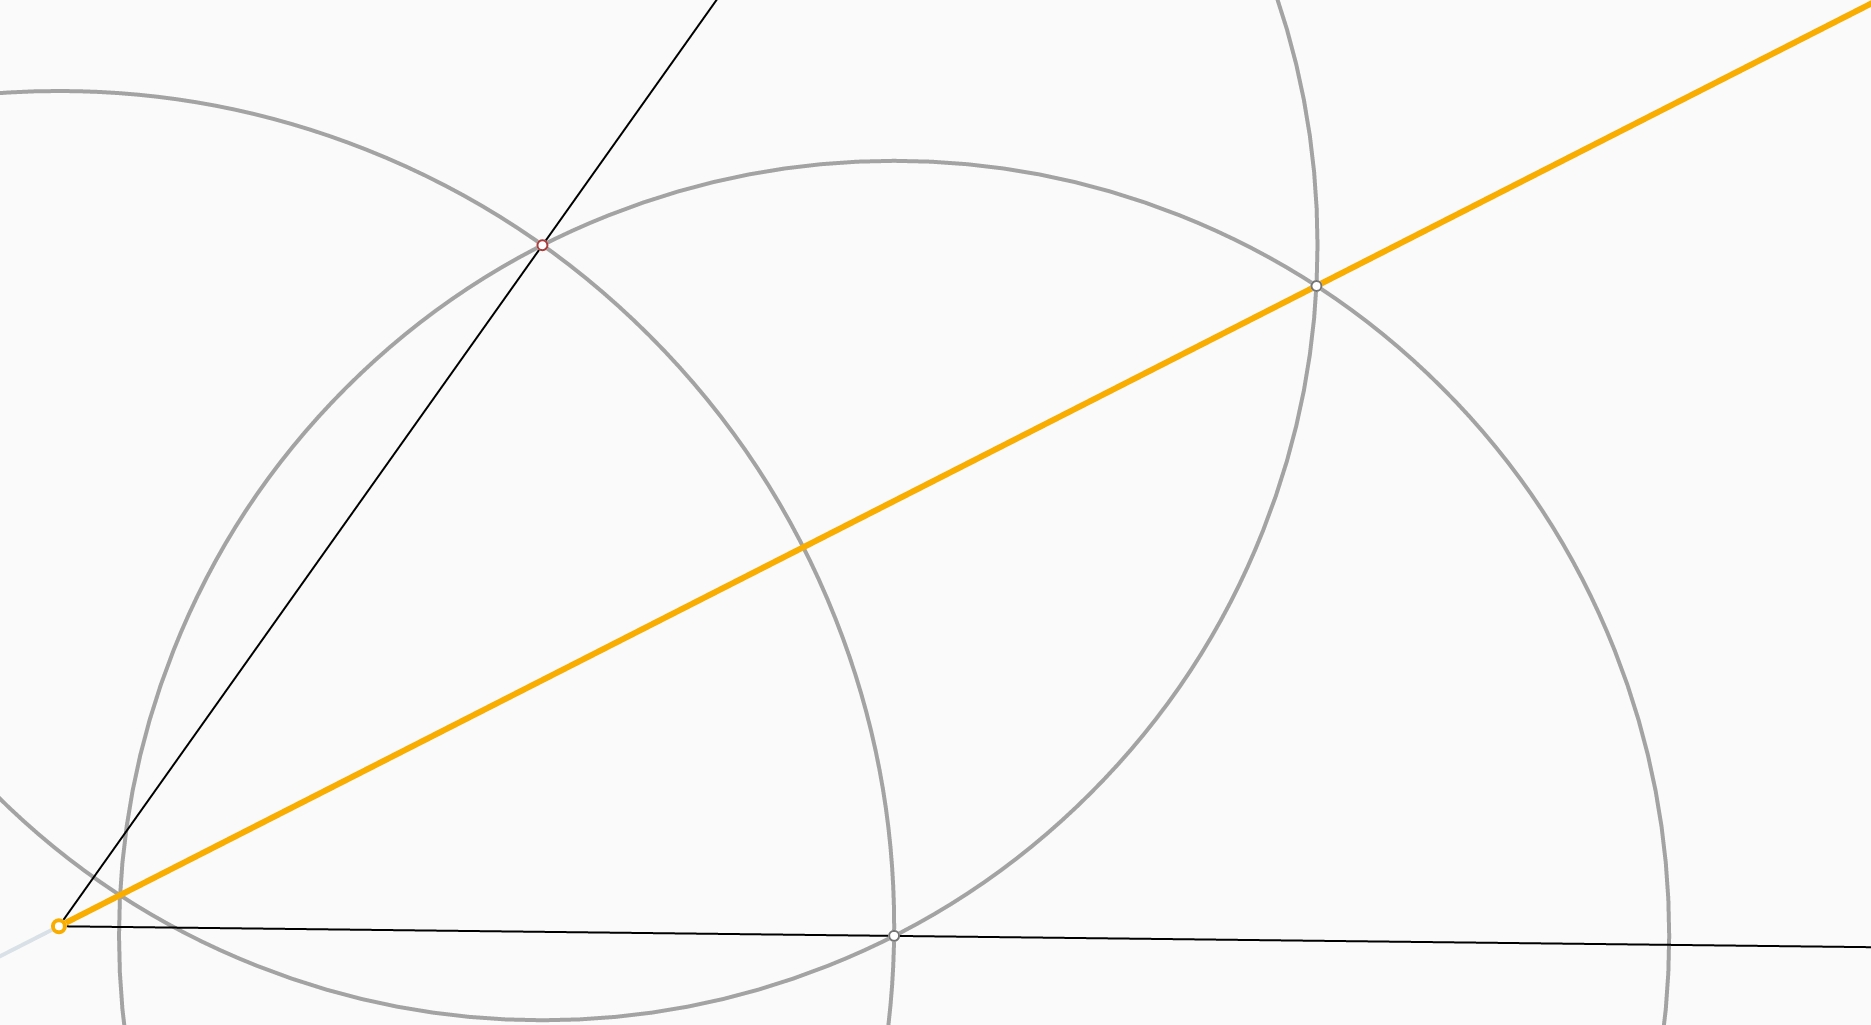
\includegraphics[width=13cm,height=7cm,keepaspectratio]{./Pictures/Winkelhalbierende.png}


    Winkelhalbierende eines Winkels:
    elementare Schritte:
    \begin{enumerate}
        \item einen Punkt definieren (-beliebig oder - Schnittpunkt von Linien)
        \item mit Zirkel Abstand von 2 Punkten abgreifen
        \item mit Zirkel einen Kreis um einen bestimmten Punkt zeichnen
        \item Zwei Punkte mit dem Lineal verbinden
    \end{enumerate}


    \item Abakisten vs. Algorithmiker (1200 bis 1500)
    \begin{itemize}[label={-}]
        \item Abakisten rechnen mit römischen Zahlen und Abakus
        \item Algorithmiker (al Quarismi: Rechnen mit indischen / arabischen Ziffern (ursprünglich aus Indien) schriftliches Rechnen wie in der Grundschule) ~800
        \item ~1200 lateinische Übersetzung ``Dixit $\underline{\text{Algorismi}}$''  $\leftarrow$ Herkunft Wort
        \item Vereinigung um 15000 : Adam Riese (Rechnen auf den Federn und Linien)
    \end{itemize}

    \item $\underline{\text{elementare Schritte im modernen Computer:}}$ \\
    $\begin{rcases}
    \bullet & \lambda\text{-Kalkül} \\
    \bullet & \text{rekursive Funktionen (Gödel)} \\
    \bullet & \text{while-Programme} \\
    \bullet & \text{Turing-Maschinen }
    \end{rcases}$ ganz untersch. Sammlungen von elementaren Schritten
    \bigskip

    $\underline{\text{Aber}}$: die Menge der Algorithmen, die man damit implementieren kann, sind identisch!
    ``$\underline{\text{Menge der berechenbaren Funktionen}}$'' $\rightarrow$ worüber die Informatik spricht



    \item $\underline{\text{while-Programme:}}$ \\
        in verbesserter Form von allen CPUs implementiert
    \begin{itemize}[label={-}]
        \item vier Grundoperationen:
        \begin{itemize}
            \item Addition einer Konstanten : \verb|x[j] = x[i] +c| \\
            \verb|x[j] =| Inhalt der Speicherstelle j; \verb|c =| Konstante
            \item Subtraktion einer Konstanten: \verb|x[j] = x [i] - c| \\
             `` $=$'' $\rightarrow$ Zuweisung
            \item Nacheinanderausführung von Programmen P und Q $\rightarrow$ \verb|P ; Q| (erst \verb|P|, dann \verb|Q|)
            \item Schleife:  \verb|WHILE x[i] != 0 DO P DONE| \\
            Programm \verb|P| sollte \verb|x[i]| irgendwann auf \verb|0| setzen, sonst Endlosschleife $\widehat{=}$ kein Algorithmus
        \end{itemize}
    \end{itemize}


    \item erstaunlicher Fakt: alle berechenbaren Funktionen können mit nur 4 elementaren Operationen ausgedrückt werden: \\
    in Backus-Naur-Notation:


    \begin{minted}{python}
Programm ::= x[i] = x[j] + c                  # Addition einer Konstanten
         |   x[i] = x[j] - c                  # Subtraktion einer Konstanten
         |   Programm ; Programm              # Nacheinanderausfuehren
         |   WHILE x[i] != 0 DO Programm DONE # Wiederholtes Ausfuehren
    \end{minted}


    Beispiel: Addition von zwei Speicherzellen \verb|x[i]| und \verb|x[j]| \\
    Spezifikation des Algorithmus: \\
    \vspace{-12mm}
    \begin{singlespace}
    \begin{itemize}[label={-}]
        \item Vorbedingung: \verb|x[j] >= 0| \\
        \item Nachbedingung: \verb|x[i]' = x[i] + x[j]      (x[i]' = x[i] |am Ende des Alg.\verb|)|
        \item Algorithmus:      \begin{minted}{python}
        WHILE x[j] != 0 DO
        x[i] = x[i] + 1 ;
        x[j] = x[j] - 1
        DONE
                                                \end{minted}
    \end{itemize}
    \end{singlespace}

in der Praxis ist das $\underline{\text{sehr ineffizient}}$: Anzahl der Schritte $\bigO{}(x[j])$ es geht auch mit $\bigO{}(log(x[j]))$ Schritten

    \item[$\Rightarrow$] pragmatische Definition von elementaren Schritten
    \begin{itemize}[label={-}]
        \item Hardware-orientierte Definition: elementare Schritte sind alle Operationen, die die jeweilige CPU anbietet (``Assembler'' ) (``Maschinensprache'' )
        \item Software-orientierte Definition: elementare Schritte sind alle Operationen, die die Programmiersprache, inklusive ihrer Standardbibliothek, anbietet.
    \end{itemize}

\end{itemize}

\section{Was ist eine Datenstruktur?}

\begin{itemize}[label={-}]
    \item Daten sind Folgen von Bits d.h. 0/1 - Folgen \\
    \begin{center}
    $1101,0110,0110,1100$
    \end{center}
    Bitfolgen allein haben $\underline{\text{keine}}$ Bedeutung, man braucht zusätzlich eine Interpretations-Vorschrift $\widehat{=}$ ``Datenformat''
    \item Beispiele:
    \begin{itemize}[label={$\bullet$}]
        \item Interpretation als ``unsigned integer 16'' \\
        \begin{tabular}{C{5mm} C{5mm} C{5mm} C{5mm} C{5mm} C{5mm} C{5mm} C{5mm} C{5mm} C{5mm} C{5mm} C{5mm} C{5mm} C{5mm} C{5mm} C{5mm}}
            1 & 1 & 0 & 1 & 0 & 1 & 1 & 0 & 0 & 1 & 1 & 0 & 1 & 1 & 0 & 0 \\
            $\uparrow$ & $\uparrow$ & $\uparrow$ & $\uparrow$ & $\uparrow$ & $\uparrow$ & $\uparrow$ & $\uparrow$ & $\uparrow$ & $\uparrow$ & $\uparrow$ & $\uparrow$ & $\uparrow$ & $\uparrow$ & $\uparrow$ & $\uparrow$ \\
            $2^{15}$ & $2^{14}$ & $2^{13}$ & $2^{12}$ & $2^{11}$ & $2^{10}$ & $2^{9}$ & $2^{8}$ & $2^{7}$ & $2^{6}$ & $2^{5}$ & $2^{4}$ & $2^{3}$ & $2^{2}$ & $2^{1}$ & $2^{0}$ \\
            =33768 & & ... & & & & & & & & & & & & =2 & =1 \\
        \end{tabular}

        33768 + ... + 8 + 4 + 0 + 0 = 54892
        \item Interpretation als ``signed integer 16 im 2er-Komplement'' \\
        Regel:
        \begin{itemize}[label={-}]
            \item wenn das linke Bit 0 ist $\Rightarrow$ unsigned int 15
            \item wenn das linke Bit 1 ist $\Rightarrow$ negative Zahl
        \end{itemize}
        $ -10644 = \begin{cases}
        \bullet \hspace{1mm} \text{alle Bits negieren und 1 addieren} \Leftrightarrow \text{interpretiere Erg. als ``unsigned int 15''} \\
        0010100110010011 \\
        \underline{\hspace{2,65cm} + 1}\\
        \hspace{2.3mm} 010100110010100
        \end{cases}$

        Ausnahme:  \\
         \hspace*{0.5cm}negieren 0111111111111111 \\
         \hspace*{1.7cm} + $\underline{ \hspace*{2.8cm} 1}$ \\
         \hspace*{2.1cm}1000000000000000 = definiert als $-2^{15}$ \\
         \hspace*{0.5cm}(die Zahl $+2^{15}$ ist in signed int 16 nicht darstellbar)


        \item Interpretation als Windows-Zeichensatz, zwei 8-bit Zeichencodes \\
        \hspace*{3cm} $\underbrace{11010110}_{\text{``Ö''}}  \hspace*{0.5cm} \underbrace{01101100}_{\text{``l''}} \Rightarrow$ Öl

        \item   Interpretation als Gleitkommazahl ``float 16'' nach dem Standard IEEE 754 \\
        \hspace*{3cm} $\underbrace{1}_{\text{sign = s}}  \hspace*{0.5cm} \underbrace{10101}_{\text{exponent = e}} \hspace*{0.5cm} \underbrace{1001101100}_{\text{mantisse = m}} $ \\
        \hspace*{3cm} $z = (1-2*s) * 2^{e-15} * (1 + m * 2^{-10})$ \\
        \hspace*{3.28cm} $= -102.75$

        \item[] usw. (unendlich viele Interpretationen)
        \end{itemize}
    \item wichtig bei Daten in Dateien: Dateien sind Bitfolgen auf Festplatte,
    \item[] $\rightarrow$ man braucht Interpretation:
    \begin{itemize}[label={-}]
        \item nach Ende des Filename: .jpg
        \item im Internet: Mime-types (Multipurpose Internet Mail Extension): mit den Daten verknüpfte Typ-Info
        \item magic numbers am Fileanfang: 255 216 255 (sonst kein .jpg, selbst wenn Endung vorhanden $\rightarrow$ evtl. Virus)
        \item alternative Möglichkeiten, Datenstrukturen zu definieren \\
        \begin{figure}[htbp]
            \begin{minipage}[t]{6cm}
                \vspace{0pt}
                \centering
                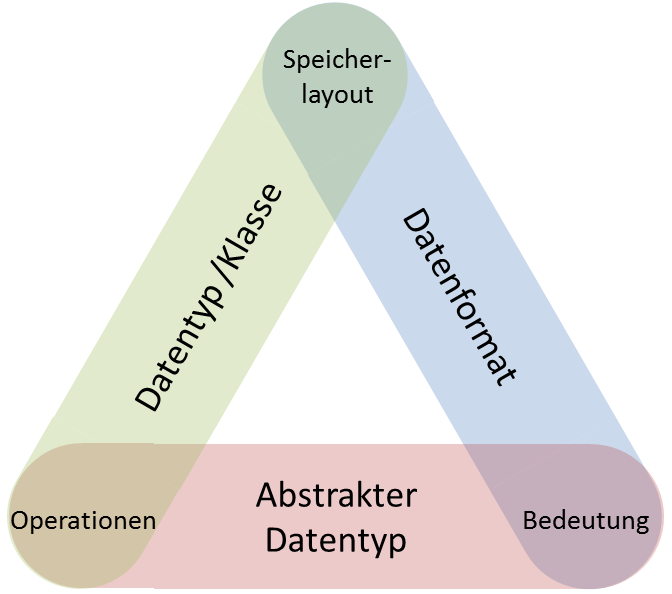
\includegraphics[width=8cm,height=8cm,keepaspectratio]{./Pictures/Dreieck.png}
                \label{fig:Bild1}
            \end{minipage}
            \hfill
            \begin{minipage}[t]{6cm}
                \vspace{0pt}
                Datenformat $\leftarrow$ Files \\
                Datentyp/Klasse $\leftarrow$ Programmiersprache \\
                Speicherlayout = Bitfolge \\
                Operationen = erlaubte Operationen \\
                Bedeutung = Interpretation \\
                String:
                \begin{itemize}[label={-}]
                    \item Bytefolge der Zeichen
                    \item Operationen: print, append, to\_lower\_case
                \end{itemize}

            \end{minipage}
        \end{figure}

        ADT $\widehat{=}$ $\underline{\text{abstract}}$ data type: Datentypen werden definiert, $\underline{\text{ohne}}$ eine spezielle Implementation als Bitfolge \\

        $\Rightarrow$ Theorie, abstrakte Spezifikation von Alg. (Pseudocode) \\
        $\Rightarrow$ Vorteil: Programmierer hat große Freiheiten für Implementation

        \end{itemize}
\end{itemize}

\section{Fundamentale Algorithmen}
stehen für (fast) alle Typen zur Verfügung
\begin{itemize}[label={$\bullet$}]
    \item Konstruktor:
    \begin{enumerate}
        \item weise einer bestimmten Speicherstelle (Bitfolge) eine Interpretation zu
        \item Initialisiere die Bitfolge mit einem festen Anfangswert (oft 0)
    \end{enumerate}
    \item[] Beispiel: in Python heißt der Konstruktor-Algorithmus wie der Datentyp \\
    \begin{minted}{python}
        i = int()       # ganze Zahl
        f = float()     # Gleitkommazahl
        l = list()      # leeres Array
    \end{minted}
    \item[] alternative Konstruktoren für andere Anfangswerte:
    \begin{minted}{python}
        j = int(2)      # ganze Zahl 2 statt 0
        a = [i, j]      # Array mit den Zahlen [0,2]
    \end{minted}

    \item Vergleiche auf Gleichheit und Identität \\
    \begin{tabular}{C{7cm} C{7cm}}
    $\downarrow$ & $\searrow$ \\
    zwei Variablen des gleichen Typs enthalten die gleiche Bitfolge & zwei Bezeichner (= Variablenname) referenzieren die gleiche Variable \\
    $\downarrow$ & $\downarrow$ \\
    $==$ & \verb|is| \\
    Negation: $!=$ & \verb|is not| \\
    \end{tabular}

    $\begin{rcases}
    \text{a} = [1,2] \\
    \text{b} = [1,2]
    \end{rcases}
    \text{``a} == \text{b''}' \text{ist wahr}; \text{``a} != \text{b''} \text{ist falsch} $ \hspace*{0.6cm}
    ``a \verb|is|  b'' ist falsch; ``a \verb|is not| b'' ist wahr \\

    Es gilt stets:
    \begin{itemize}[label={-}]
        \item ``a \verb|is| b'' wahr $\rightarrow$ ``a $== $b'' wahr
        \item ``a \verb|is| a'' und ``a $==$ a'' immer wahr
    \end{itemize}
    \item swap-Operation: Vertauschen der Bitfolgen von zwei Variablen des gleichen Typs \\
    andere Programmiersprachen: swap(a,b) \\
    Python:
    \begin{itemize}[label={}]
        \item Mehrfachzuweisung: a, b = b, a
        \item Beispiel-Verwendung: Sortieren
    \end{itemize}
\end{itemize}


\subsection*{Referenzsemantik vs. Wertsemantik}
    \begin{itemize}[label={-}]
        \item Wofür steht ein Variablenname in einer Programmiersprache?
        \item Was genau bewirkt die Zuweisung an einen Variablennamen?
        \item Analogie:
    \end{itemize}
    \begin{tabular}{C{7cm} C{7cm}}
    Bookmarks im Internet \hspace*{1cm}vs. &  Download einer Seite \\
    $\Downarrow$ & $\Downarrow$ \\
    URL, mit der man eine Seite wieder aufrufen kann & lokale Kopie der Seite
    kann wieder aufgerufen werden \\
    $\underline{\text{aber:}}$ es könnte auch eine neue sein & $\underline{\text{aber:}}$ könnte veraltet sein \\
    & \\
    URL $\widehat{=}$ Referenz auf die Seite (ähnlich der Adresse einer Wohnung) & Kopie \\
    $\widehat{=}$ & $\widehat{=}$ \\
    Referenzsemantik & Wertsemantik \\
     & \\
    $ \underline{\text{Python:}}$ für alle anderen Typen & Zahlen(int, float, boolean, string)\\
    \begin{minted}[breaklines=false, linenos=false]{python}
    i = [1,2]
    j = i           #j=[1,2]
    i = [0] = 3     #i=[3,2] j=[3,2]
    \end{minted}
                                                         &
    \begin{minted}[breaklines=false, linenos=false]{python}
    i=int(2)
    j=i             # j==2
    i=3             # j==2,
    \end{minted}
    \\
    i und j sind nur alternative Namen für die selbe Speicherstelle & i und j verweisen auf verschiedene Speicherstellen \\
    \end{tabular}




\subsection*{Freiheitsgrade bei der Datenstruktur-Definition}

\begin{itemize}[label={$\bullet$}]
    \item Datenformat: u int8 (8 bit, als unsigned integer interpret.)
    \begin{itemize}[label={-}]
        \item Speicher \& Interpretation festgelegt
        \item Operation: Addition: -Funktionsname ``add'', ``plus'', ``+''
        \item Implementation:  \\
        \hspace*{0.5cm}00000001 \\
        \hspace*{0.05cm} + $\underline{ 00000001}$ \\
        \hspace*{0.5cm}00000010\\

        \hspace*{0.5cm}11111111 $\widehat{=}$ 255 \\
        \hspace*{0.05cm} + $\underline{00000001}$ \\
        \hspace*{0.25cm} 100000000 $\widehat{=}$ 256 $\Rightarrow$ 9 bit ?? \\

        \item Konvention:
        \begin{itemize}[label={-}]
            \item es passiert \emph{nichts}, bleibt 255 \\
            Keine gute Idee, z.B. Kommutativität :( \\
            Beispiel: \verb| i = j + k| wenn j und k vertauscht werden: Was bleibt dann erhalten?
            \item Fehlermeldung: ``Zahl zu groß'' \\
            suboptimal, weil es evtl. zu oft zu Programmabbrüchen kommt
            \item Berechnung ``modulo 256'' \\
            $(255+1)mod256 = 0$ \\
            man rechnet zyklisch \\
            funktioniert ebenso im negativen Bereich
            (CPU: Übertrag der letzten Addition wird gelöscht)
        \end{itemize}
    \end{itemize}
\end{itemize}



\chapter*{2 Container}
\addcontentsline{toc}{chapter}{2 Container}
\begin{itemize}[label={-}]
    \item Datenstrukturen, die andere Datenstrukturen enthalten
    \item wichtig, weil Computer benutzt werden, wenn man dieselbe Operation sehr $\underline{\text{häufig}}$ ausführen will
\end{itemize}
$\underline{\text{Beispiele:}}$
\begin{itemize}[label={-}]
    \item RGB Pixel: 3 Helligkeitswerte für Rot, Grün, Blau
    \item Bild: Container von RGB Pixeln (1024x1024)
    \item Video: Folge von Bildern (20 fps)
\end{itemize}
Grundprinzip: DS können geschachtelt werden, um mächtigere DS zu erzeugen



\section*{2.1 Abstrakte Container – Datentypen}
\addcontentsline{toc}{section}{2.1 Abstrakte Container – Datentypen}

Interpretation \& Operation (Bit-Repräsentation ist dem Programmierer überlassen) \\

Notation: Operationen werden durch Vor- und Nachbedingung spezifiziert, dabei ist \verb|x| die DS vor der Operation, \verb|x'| nach der Operation \\

\subsection*{3 Arten von Operationen: }
\begin{itemize}[label={-}]
    \item Konstruktoren: erzeugen eine neue DS mit definiertem Anfangszustand
    \item Accessoren: aktuellen Zustand (=Inhalt des Containers) abfragen
    \item Modifizierer: aktuellen Zustand ändern
\end{itemize}


\section*{2.2 Grundlegende Container}
\addcontentsline{toc}{section}{2.2 Grundlegende Container}

    \subsection*{2.2.1 Array}
    \addcontentsline{toc}{subsection}{2.2.1 Array}
    speichert Objekte im Speicher hintereinander ab \\

    \begin{tabular}{| C{1cm} | C{1cm} | C{1cm} | C{1cm} |C{1cm} | C{1cm}| C{1cm} |C{1cm}| C{1cm}| C{1cm}| }
        \hline
        Ob1 & Ob2 & Ob3 & ... & & & & & & ObN \\ \hline
    \end{tabular} \\

    Zugriff auf Objekte erfolgt über den Index $\widehat{=}$ laufende Nummer Position im Array \\

    Denkschulen:
    \begin{itemize}
        \item zero-band indexing (C, C++, Python) \\
        \fbox{0-based: 0, 1, ..., N-1 (N = Arraygröße)}
        \item one-based indexing (Fortran, Matlab, Julia)\\
        1-based: 1, 2, ..., N
    \end{itemize}

    ADT: \\
    \begin{tabular}{C{5cm} C{5cm} C{5cm}}
        Op & Bedeutung & Axiom \\ \hline
        \verb| a = new_array(size, initial)| & Konstruktor & \verb|len(a) == size| \\
        & & $\forall i \in [0, size - 1]$: \\
        & & \verb|get(a,i) == initial| \\ \hline
        \verb|v=get(a,i)| & Zugriff auf Element i & Vorbedingung: $i \in [0, size-1]$ \\
        & & Nachbedingung: \verb| v ==| i-tes El. \\
        & & \verb|a' == a| \\ \hline
        \verb|set(a, i, v)| & Setzen des i-ten Elements & Vorbed: $ i \in [0, size-1]$ \\
        & & Nachbed.: \verb|get(a',i) == v| \\
        & & $\forall k \neq i:$ \verb|get(a',k) == get(a,k)| \\
    \end{tabular}

    in Python:
    \begin{itemize}[label={}]
        \item get $\Rightarrow$ \verb|__getitem__|
        \item set $\Rightarrow$ \verb|__setitem__|
        \item[$\bullet$] Punktsyntax: \verb|get(a,i)| $\Rightarrow$ \verb|a.__getitem__(i)| \\
        ``\_\_getitem\_\_'' ist Methode der Klasse
        \item[$\bullet$] Index-Notation \\
        \verb|get(a,i)| $\Rightarrow$ \verb|v = a[i]| (falls auf der rechten Seite der Zuweisung) \\
        \verb|set(a,i,v)| $\Rightarrow$ \verb|a[i] = v|
        \item[$\bullet$] Konstruktor: \verb|new_array| $\Rightarrow$ list \\
        ($\underline{\text{nicht}}$ mit verketteter Liste $\underline{\text{verwechseln}}$)
    \end{itemize}

    \subsection*{2.2.2 Stack}
    \addcontentsline{toc}{subsection}{2.2.2 Stack}
    $\widehat{=}$ Stapel (z.B. von Bierkästen) \\
    nur der oberste Kasten ist leicht zugreifbar \\

    \begin{tabular}{C{5cm} C{5cm} C{5cm}}
        Op & Bedeutung & Axiome \\ \hline
        \verb|s = new_stack()| & Konstruktor & \verb|len(s) == 0| \\
        \verb|len(s)| & Abfrage der Größe & (= aktuelle Anzahl der Elemente) \\
        \verb|push(s,v)| & Element v am Ende anhängen (oben drauf stapeln) & $\begin{cases}
        \verb|len(s') == len(s) + 1| \\
        \verb|top(s') == v|
        \end{cases}$ \\
        \verb|top(s)| & Abfragen des obersten Elements & \\
        \verb|pop(s)| & Entfernen des obersten/letzten Elements & $\begin{cases}
        \verb|s'= pop(s, push(s,v))| \\
        \verb|s' == s| \end{cases}$ \\
    \end{tabular} \\

    in Python: die DS ``list'' ist auch ein Stack
    \begin{itemize}
        \item \verb|push(s,v)| $\Rightarrow$ \verb|s.append(v)|
        \item \verb|pop(s)| $\Rightarrow$ \verb|s.pop()|
        \item \verb|top(s)| $\Rightarrow$ \verb|s[-1]|
    \end{itemize}
    Konventionen in Python: negative Indizes vom Ende gerechnet
    \begin{itemize}[label={}]
        \item \verb|s[i]| (i positiv): normaler Zugriff
        \item \verb|s[i]| (i negativ): \verb|s[len(s)+i]|
        \item \verb|s[-1]    s[len(s)-1]|
    \end{itemize}

    Stackverhalten: LIFO ``last in – first out''

    \subsection*{2.2.3 Queue}
    \addcontentsline{toc}{subsection}{2.2.3 Queue}
    $\widehat{=}$ Warteschlange (z.B. Eisdiele) \\

    FIFO ``first in – first out'' \\
    ``first come - first serve'' \\

    \begin{tabular}{C{5cm} C{5cm} C{5cm}}
        Op & Bedeutung & Axiome \\ \hline
        \verb|push(q,v)| & v am Ende anhängen (wie beim Stack) & \\
        \verb|first(q)| & das erste Element (gegensatz Stack: \verb|top(s)| $\Rightarrow$ letztes Element) & \\
        \verb|pop(q)| & entferne das $\underline{\text{erste}}$ Element (geg. Stack: das letzte El.) & \\ \hline
    \end{tabular}

    in Python:
    $\begin{rcases}
        \verb|first(q)| \Rightarrow \verb|q[0]| \\
        \verb|pop[q]| \Rightarrow \verb|q.pop(0)|
        \end{rcases}$
        Funktion von ``list'' \\

        \subsection*{2.2.4 Deque}
        \addcontentsline{toc}{subsection}{2.2.4 Deque}
        $\widehat{=}$ double ended Queue $\widehat{=}$ DS gleichzeitig Stack und Queue \\

        \verb|pop_front()| $\widehat{=}$ erstes Element entfernen $\widehat{=}$ Queue \\
        \verb|pop_back()| $\widehat{=}$ letztes Element entfernen $\widehat{=}$ Stack \\

        \subsection*{2.2.5 Assoziatives Array}
        \addcontentsline{toc}{subsection}{2.2.5 Assoziatives Array}
        $\widehat{=}$ Dictionary $\widehat{=}$ in Python ``dict'' \\

        statt Indizes aus $\mathbb{N}_{0}$ (natürliche Zahlen) sind $\underline{\text{beliebige}}$ Schlüssel erlaubt. \\

        typische Fälle:
        \begin{itemize}[label={-}]
            \item natürliche Zahlen, die nicht in \verb|[0, N-1]| liegen \\
            z.B. Matrikelnummern \\
            \verb|a[1359742]| $\Rightarrow$ ``Fritz Schulze''
            \item strings, z.B. Namen \\
            \verb|alda_noten["Fritz Schulze"]| $\Rightarrow$ 1.0
        \end{itemize}
        die Schlüsselworte werden automatisch (versteckt vor Programmierer) in die eigentlichen Speicherindizes umgerechnet \\

        \subsection*{2.2.6 Ausblick: Prioritätswartescchlangen}
        \addcontentsline{toc}{subsection}{2.2.6 Prioritätswarteschlangen}
        \verb|a.top(), a.pop()| greifen zu / entfernen das Element mit $\underline{\text{höchster Priorität}}$\\

        Stack und Queue sind Spezialfälle: \\
        neuestes bzw. ältestes Element haben höchste Priorität \\


        \subsection*{Anwendungen von Queue und Stack}
        \begin{itemize}
            \item Queue: Drucken-Warteschlange
            \item Stack:Undo-Funktionalität in Textprogrammen
        \end{itemize}

        \begin{tabular}{C{5cm} | C{5cm} | C{5cm}}
            Aktion des Benutzers & undo-stack u & redo-Stack v \\ \hline
            $a_1$ & \verb|u.push(a1)| & \\
            $a_2$ & \verb|u.push(a2)| & \\
            $a_3$ & \verb|u.push(a3)| & \\ \hline
            undo & \verb|undo(u.top())| $\Rightarrow a_3$ rückgängig & \\
            & \verb|u.pop()| & \verb|v.push(u.top())|\\ \hline
            undo & \verb|undo(u.top())| $\Rightarrow a_2$ rückgängig & \\
            & \verb|u.pop()| & \verb|v.push(u.top())|\\ \hline
            redo & & \verb|do (v.top())| $\Rightarrow$ $a_2$ wiederherstellen \\
            & \verb|u.push(v.top())| & \verb|v.pop()| \\ \hline
            $a_4$ & \verb|u.push(a4)| & \verb|v.clear()| \\
            $\vdots$ & $\vdots$ & $\vdots$ \\
        \end{tabular}




        \chapter{Sortieren}
        Warum?
        \begin{itemize}
            \item viele Konzepte des Algorithmen-Design und -Vergleichs werden sehr anschaulich
            \item sortierte Daten braucht man oft in der Praxis, z.B. zum schnellen Suchen
            \item aber: man muss sortieren heute selten selbst implementieren, weil alle Programmiersprachen das schon anbieten \\
            \hspace*{1cm} \verb|sort(a)|
        \end{itemize}

        \textbf{Spielregeln}:
        \begin{enumerate}
            \item Die Daten liegen in einem Array: \verb|a| \\
            $\Rightarrow$ Der Alg. darf aufrufen: \\
        \end{enumerate}
        \vspace*{-5mm}
        \begin{minted}{python}
            N = len(a)              # Laenge von a
            v = a[i]                # Lesen von El.i
            a[i] = v                # Schreiben von El.i
        \end{minted}

        mit $i \in [0, N-1]$ \\
        $\Rightarrow$ Der zu sortierende Datentyp ($\widehat{=}$ Elemente des Arrays) unterstützen in Vergleichsfunktion, meist ``$<$'' \\
        $a[i] < a[k] \Rightarrow$ \verb|True oder False| \\

        Der Vergleich muss die mathematischen Anforderungen einer \emph{totalen Ordnung} erfüllen \\


        Eine totale Ordnung ist antisymmetrisch, transitiv, reflexiv, total \\
        Elemente $a,b,c,...$ und die Relation ``$\leq$'': $a \leq b \rightarrow$ \verb|t, f| \\
        \begin{itemize}
                \item total: man kann beliebige Elementpaare vergleichen \\
                $a \leq b$ liefert immer \verb|t oder f| \\
                (Gegenteil: Halbordnung: manche Elemente nicht vergleichbar
                $a\leq b$ liefert \verb|t oder f oder "unknown"|)

                \item antisymmetrisch: $a \leq b \land b \leq a \Rightarrow a == b$
                \item transitiv: $ a \leq b \land b \leq c \Rightarrow a \leq c$
                \item reflexiv: (folgt aus den anderen): $a \leq a$ immer \verb|true|
        \end{itemize}

            Frage: Angenommen $a \leq b$ ist definiert, aber der Sortieralgorithmus braucht $a < b$. \\
            Kann man $a < b$ implementieren, indem man nur logische Operationen $\land \lor \lnot$ sowie $\leq$ verwendet? \\

            Antwort: $a < b \Leftrightarrow \lnot(b \leq a)$ \\

            Hausaufgabe: Wie bekommt man $>, \geq, ==, !=$ \\

            \section{Selection Sort}

            \begin{minted}{python}
def selection_sort(a):
    N = len(a)
    for i in range(N-1):        # i ist die Arrayposition, die wir sortieren wollen
        m = i                   # m ist unsere aktuelle Meinung,
                                # wo das kleinste rechts von i steht
        for k in range(i+1, N):
            if a[k] < a[m]:
                m = k           # Meinung korrigieren
                                # a[m] ist jetzt das kleinste Element rechts von i
        a[i], a[m] = a[m], a[i] # vertauschen
            \end{minted}
            \begin{itemize}
                \item Datenobjekte haben oft mehrere Eigenschaften, nach denen man sortieren kann. \\
                Studenten: Sortieren nach Alter, Alda-Noten, ... \\
                hier: nach Zahl oder Farbe\\
                sortiere jetzt nach Farbe: orange $<$ rot$ <$ blau $<$ schwarz

                \textbf{Stabiliät der Sortierung}:
                \begin{itemize}
                    \item Anfangs ist das Array nach Kriterium 1 sortiert (``Zahl'')
                    \item Wir sortieren nun nach Kriterium 2 (``Farbe''), aber es gibt Elemente, die dabei den gleichen Wert haben
                    \item Sortieralgorithmus ist \emph{stabil}, wenn die Ordnung 1 erhalten bleibt, über Elementen mit identischem Wert 2
                \end{itemize}
            \end{itemize}
            $\Rightarrow$ Selection Sort nicht stabil \\

            \section{Insertion Sort}
            ähnlich einfach wie Selection Sort, aber \emph{stabil}
            \begin{itemize}
                \item Beobachtung: Insertion Sort ist für \emph{kleine Arrays} (N $<$ 30) der schnellste Sortieralgorithmus \\
            \end{itemize}
            \begin{minted}{python}
def insertion_sort(a):
    N = len(a)
    for i in range(N):
        current = a[i]
        k = i
        while k > 0:
            if current < a[k - 1]:
                a[k] = a[k - 1]
            else:
                break
            k = k - 1
    a[k] = current
            \end{minted}

            Welche Laufzeit benötigen Selection und Insertion Sort?
            \begin{itemize}
                \item Wie misst man das unabhängig davon, ob man einen schnellen oder langsamen Computer hat, oder wie groß N ist?
                \item 2 Lösungen: Zähle a Anzahl der Vergleiche $a < b$, b Anzahl der Vertauschungen \\
            \end{itemize}

        \begin{tabular}{C{3cm} | R{5cm}}
                i & Anzahl der Schritte in der Schleife $\widehat{=}$ Anzahl Vergleiche \\ \hline
                0 & $k \in [1, N-1] \widehat{=} N-1$ S. \\
                1 & $[2, N-1] \widehat{=} N-2$ S. \\
                2 & $\widehat{=} N-3$ S. \\
                $\vdots$ & \\
                $N-2$ & $[N-1, N-1] \widehat{=} 1$ S. \\
        \end{tabular}

    $\Rightarrow$ die totale Anzahl Vergleiche: \\
    $T = (N-1)+(N-2)+(N-3)+...+2+1$\\

    \fbox{$= \frac{N(N-1)}{2} \approx \frac{N^2}{2}$}\\

    Anzahl Vertauschungen: $ V = N-1 < T$


    \subsection*{Elementare Sortierverfahren}
    iteriere mit i über alle Arrayelemente

    \begin{itemize}
        \item Selection Sort: finde das $\underline{\text{kleinste}}$ Element $\underline{\text{rechts}}$ von i und bringe es auf Position i
        \item Insertion Sort: Finde die passende $\underline{\text{Lücke}}$ $\underline{\text{links}}$ von i, wo Element a[i] einsortiert werden muss

    \end{itemize}

    \subsection{Aufwand beim Sortieren}
    Aufwand beim Sortieren: Anzahl der Vergleiche $a[i] < a[k]$ und/oder Anzahl der Vertauschungen $a[i],a[k] = a[k], a[i]$

    \begin{itemize}
        \item bei Selection Sort: Anzahl Vergleiche $V = \frac{N(N-1)}{2}$
        \item bei Insertion Sort: Unterscheide drei Fälle:
        \begin{itemize}
            \item günstigster Fall: Array schon sortiert
            \item ungünstigster Fall: Array umgekehrt sortiert (absteigend statt aufsteigend)
            \item typischer Fall: Array zufällig angeordnet
        \end{itemize}
        \item alle drei Fälle haben unterschiedliches V! \\
        (bei Selection Sort: V immer gleich)

    \end{itemize}

    \begin{minted}{python}
def insertion_sort_1(a):
    N = len(a)
    for i in range(1, N):
        k = i
        while k > 0:
            if a[k] < a[k - 1]:
                a[k - 1], a[k] = a[k], a[k - 1]
            else:
                break
            k = k - 1
    \end{minted}

    $\Rightarrow$ für kleine N der schnellste Algorithmus \\
    \vspace*{-5mm}
    \begin{enumerate}
        \item günstigster Fall: Array ist sortiert, d.h. der Vergleich (*) liefert immer sofort ``False" '$\Rightarrow$ while-Schleife hat nur 1 Iteration \\
        $\Rightarrow$ ein Vergleich pro i $\Rightarrow$\fbox{$V = N-1$}
        \item ungünstigster Fall: Array umgekehrt sortiert $\Rightarrow$ Vergleich (*) liefert immer ``True'' $\Rightarrow$ while-Schleife muss immer bis zum Ende (k=0) durchlaufen werden $\Rightarrow$ i Vergleiche für jedes i \\
        $V=1+2+3+...+(N-1)=$ \fbox{$\frac{N(N-1)}{2} = V$} $\approx$ \fbox{$\frac{N^2}{2}$}
        \item typischer Fall: Array zufällig $\Rightarrow$ im $\underline{\text{Mittel}}$ wird die while-Schleife zur Hälfte durchlaufen $\Rightarrow$ \fbox{$V = \frac{N(N-1)}{4}$} $\approx$ \fbox{$\frac{N^2}{4}$}
    \end{enumerate}


    Einwurf: \\
    swap braucht mindestens 3 Zuweisungen: \\
    \hspace*{5mm} swap(a,b) : tmp = a, a = b, b = tmp \\
    in Python: sogar 4 a,b = b,a $\widehat{=}$ t1=a, t2=b, b=t1, a=t2


    \subsection*{Sortieren nach dem Teile-und-Herrsche-Prinzip}

    \begin{itemize}
        \item elementare Alg. brauchen im typischen Fall $V= c * N^2$ Vergleiche für eine Konstante c $\Rightarrow$ sie sind für große N langsam
        \item bessere Alg.: teilen das Sortierproblem in Unterprobleme, die getrennt sortiert und dann effizient zusammengesetzt werden.

    \end{itemize}

    \section{Merge Sort}

    \begin{itemize}
        \item Operation merge: Setze ein großes Array aus zwei sortierten Teilarrays zusammengesetzt
    \end{itemize}

    \begin{minted}{python}
def merge(l, v):  # l,r: sortierte Teilarrays
    a = []  # leeres Array fuer das Ergebnis
    i, k = 0, 0
    Nl, Nr = len(l), len(r)
    while i < Nl and k < Nr:
        if l[i] <= r[k]:
            a.append(l[i])
            i = i + 1
        else:
            a.append(r[k])
            k = k + 1

    a = a + l[i:Nl] + r[k:Nr]  # Rest von l bzw. r an a anhaengen
    return a
    \end{minted}


    \verb|r[k : Nr]| entspricht: \\
    \begin{minted}{python}
    while k < Nr:
        n.append(r[k])
        k = k+1
    while i < Nl:
        n.append(l[i])
        i = i+1
    \end{minted}


    \begin{itemize}
        \item um l und r zu sortieren, wendet man das gleiche Prinzip $\underline{\text{rekursiv}}$ auf die linke bzw. rechte Hälfte des Arrays an:
    \end{itemize}

    \begin{minted}{python}
def merge_sort(a):
    N = len(a)
    if N <= 1:                            # leeres Array oder mit 1 Element
        return a                          # ist automatisch sortiert
    else:
        l = a[0:N//2]                     # N//2 = "floor division", rundet ab
        r = a[N//2 : N]
        l_sorted = merge_sort(l)          # teile-und-herrsche
        r_sorted = merge_sort(r)
        a_sorted = merge(l_sorted, r_sorted)
        return a_sorted
    \end{minted}

        \textbf{Laufzeit von merge sort:} \\
        \begin{itemize}
            \item Wie tief ist der Baum, der bei der Ausführung entsteht?
        \end{itemize}

        Beispiel für $N=8$


        \begin{center}
            \begin{tikzpicture}[scale=0.9,level/.style={sibling distance=60mm/#1}]
            \node[circle, draw] (a) {N}
            child {node [circle, draw] (b) {N/2}
                child {node [circle, draw] (c) {N/4}
                    child {node [circle, draw] (d) {1}}
                    child{node [circle, draw] (e) {1}}}
                child {node [circle, draw] (f) {N/4}
                    child {node [circle, draw] (g) {1}}
                    child {node [circle, draw] (h) {1}}}
            }
            child {node [circle, draw] (i) {N/2}
                child {node [circle, draw] (j) {N/4}
                    child {node [circle, draw] (k) {1}}
                    child {node [circle, draw] (l) {1}}}
                child {node [circle, draw] (m) {N/4}
                    child {node [circle, draw] (n) {1}}
                    child {node [circle, draw] (o) {1}}}
            };
            \end{tikzpicture}
        \end{center}

        $8 = 2^3 \Rightarrow$: \fbox{$M + 1 = \text{Tiefe} = \ceil{log_2 N}$} \\

        Wie viele Vergleiche braucht man pro Ebene? \\

        \hspace*{5mm} $\rightarrow$ Ebene 1: Zwei Arrays der Länge N/2 \\
        \hspace*{7mm} $\Rightarrow$ merge vergleicht immer die ersten Elemente von l und r \\
        \hspace*{5mm} ungünstigster Fall: das kleinste Element ist abwechselnd links und rechts $\Rightarrow$ (N-1) Vergleiche $\approx$ N Vergleiche \\

        dazu kommen die Vergleiche für das Sortieren der Teilarrays l und r \\

        \hspace*{5mm} $ \Rightarrow  V(N)= \underbrace{N}_{\approx N-1} + \underbrace{2}_{\text{2 Arrays}}* \underbrace{(N/2)}_{\text{der Länge N/2 sortieren}} $ \\

        \hspace*{19.5mm} $= N + \underbrace{[\frac{N}{2} + 2 * V(\frac{N}{4})]}_{\text{l sortieren}} + \underbrace{[\frac{N}{2} + 2 * V(\frac{N}{4})]}_{\text{r sortieren}}$ \\

        \hspace*{19.5mm} $= N + (\frac{N}{2} + \frac{N}{2}) + 4 * [\frac{N}{4} + 2 * V(\frac{N}{8})] $\\

        \hspace*{19.5mm} $= N + \underbrace{(\frac{N}{2} + \frac{N}{2})}_{N} + \underbrace{4 * (\frac{N}{4}}_{N}) + \cdots $\\

        \hspace*{19.5mm} $= N + N + N + \cdots + N$

        \begin{itemize}[label={$\Rightarrow$}]
            \item pro Zerlegungsebene N Vergleiche (bzw. Zuweisungen)
            \item da es $\ceil{log_2 N}$ Ebenen gibt, ist die Gesamtzahl der Vergleiche
        \end{itemize}

        \hspace*{5mm} \fbox{$V = N * \ceil{log_2 N}$} $<< \frac{N^2}{4}$ für große N \\


        günstiger Fall: Array bereits sortiert \\

        $\Rightarrow$ bei merge werden zuerst alle Elemente von l gewählt, dann r an das Ergebnis-Array angehängt \\

        $\Rightarrow$ man braucht nur halb so viele Vergleiche wie im ungünstigen Fall \\

        \hspace*{5mm} $V= \frac{N}{2} \ceil{log_2(N)} = c N * \ceil{log_2(N)}$ \\

        unterscheidet sich nur durch Konstante c $\widehat{=}$ unwichtig \\

        \begin{itemize}
            \item Merge Sort ist $\underline{\text{stabil}}$, wenn bei Gleichheit l[i] == r[k] immer das $\underline{\text{linke}}$ Element gewählt wird
            \item Python's list.sort()-Funktion verwendet merge sort wegen der Stabilität\\
            $\underline{\text{aber}}$: hochoptimiert, d.h. häufige Spezialfälle (bereits sortiert, umgekehrt sortiert) werden abgefangen und schneller implementiert
        \end{itemize}

    \section{Quick Sort}

    \begin{itemize}
        \item Standard-Algorithmus für Sortieren, z.B. in vielen Implementationen von C++:  std::sort() \\
        (optimierte Kombination von Quick Sort mit heap sort \& insertion sort)
        \item Nachteil von merge sort: es braucht temporären Speicher zum Anlegen der gemergten Arrays
        \item besser: in-place $\widehat{=}$ sortieren erfolgt im Originalarray \\
        $\Rightarrow$ quick sort
        \item Idee: Funktion ``partition'': wähle Pivot-Element und sortiere es an die korrekte Stelle $\Rightarrow$ alle linken sind kleiner, alle rechten größer, aber nicht untereinander sortiert
    \end{itemize}

    \begin{minted}{python}
def partition(a, l, r):       # l: linke Grenze des zu sortierenden Bereichs
    pivot = a[r]              # r: rechte Grenze
    i = l, k = r - 1
    while True:               # Endlosschleife -> wird unten per "break" verlassen
        while i < r and a[i] <= pivot: # suche Element > pivot
            i = i+1
        while k > l and a[k] >= pivot: # suche Element < pivot
            k = k - 1
        if i < k :
            a[i], a[k] = a[k}, a[i]    # tausche oder beende Schleife
        else:
            break
    a[r] = a[i]
    a[i] = pivot              # bringe pivot an richtige Pos.
    return i                  # pivot-Position fuer Rekursion

def quick_sort(a):
    quick_sort_impl(a, 0, len(a)-1)
    (return a)

def quick_sort_impl(a, l, r):
    if r <= l :            # a[l : r + 1] hat hoechstens ein Element -> schon sortiert
        return (None)
    k = partition(a, l, r) # k ist korrekte Position des Pivot
    quick_sort_impl(a, l, k-1)  # rekursiv links
    quick_sort_impl(a, k+1, r)  # rekursiv rechts
    \end{minted}

    \subsection*{Laufzeit von Quick Sort}
    \begin{itemize}
        \item günstiger Fall: das Pivot ist bei jedem Aufruf immer der Median des Teilarrays ($\widehat{=}$ Element in der Mitte, nach partition())\\
        $\Rightarrow$ die verbleibenden Teilarrays sind ungefäht gleichgroß \\

        Rekursionsformel: allg. Prinzip: $\underbrace{C(N)}_{\text{totale Laufzeit für Größe N}} = \underbrace{A(N)}_{\text{Laufzeit im aktuellen Teilarray}} + \underbrace{R(N)}_{\text{Laufzeit für rekursive Aufrufe}}$\\

        \verb|C(quick_sort_imp(N)) = C(partition(N)) + C(qsi(links)) + C(qsi(rechts))| \\

        \vspace*{-5mm}
        $C_g(N) \approx (N+1)+C_g(\frac{N}{2} -1) + C_g(\frac{N}{2} -1)$\\

        \vspace*{-5mm}
        $\approx N + 2+ C_g(\frac{N}{2}) = N*\ceil{log_2(N)}$

        \item ungünstiger Fall: Pivot ist immer am Rand, d.h. partition() verändert die Position des Pivots nicht $\widehat{=}$ Array war schon sortiert \\
        $C_u(N) = \underbrace{(N+1)}_{\text{partition}} + \underbrace{C_u(N - 1) + C_u(0)}_{\text{Rekursion}} \hspace*{1cm} C_u(0)=0$ \\

        \vspace*{-5mm}
        $ = (N+1) + [N + C_u(N-2)]$ \\

        \vspace*{-5mm}
        $= (N+1) + N + \biggl\lbrack(N-1) + C_u(N-3)\biggr\rbrack$ \\

        \vspace*{-5mm}
        $ = (N+1) + N + ... + 1 = \frac{(n+2)(N+1)}{2} \approx \frac{N^2}{2}$ \\
        \vspace*{-2mm}
        $\Rightarrow$ so langsam wie selection sort $\Rightarrow$ wir müssen den ungünstigen Fall verhindern

        \item typischer Fall: Array ist zufällig sortiert \\
        $\Rightarrow$ jede Position zwischen l und r ist mit gleicher Wahrscheinlichkeit die Position des Pivot nach partition() \\
        $\Rightarrow$ wir verwenden den Mittelwert des Aufwands in der Rekursionsformel \\
        \[C_t(N) = (N+1) + \frac{1}{N}  \hspace*{-9mm} \underbrace{\underbrace{\sum_{k=1}^N}_{\text{mögliche Pos. des Pivots}}\hspace*{-9mm} [C_t(k-1) + C_t(N-k)]}_{= 2 \sum_{k=1}^N C_t(k-1)} \]\\
        \vspace*{-6mm}
        \[N * C_t(N) = (N+1) * N + 2 \sum_{k=1}^N C_t(k-1)\] \\
        \vspace*{-6mm}
        \[ \begin{rcases}(N-1) C_t(N-1) = N*(N-1) + 2 & \\
         N * C_t(N) = (N+1) * N + 2 \sum_{k=1}^{N-1} C_t(k-1) & \end{rcases} - \]\\
         \vspace*{-6mm}
        \[N* C_t(N) - (N-1) C_t(N-1) = (N+1)N - N(N-1) + 2 C_t(N-1) \] \\
        \vspace*{-9mm}
        \[ N * C_t(N) = (N+1) * C_t(N-1) + 2N \hspace*{4mm} \big| :N\] \\
        \vspace*{-9mm}
        \[ C_t(N) = \frac{N+1}{N} C_t(N-1) + 2* \frac{N+1}{N+1} \] \\
        \vspace*{-9mm}
        \[ (N+1) \biggl\lbrack \frac{1}{N} C_t(N-1) + \frac{2}{N+1}\biggr\rbrack \] \\
        $ C_t(N-1)$ sukzessive expandieren \\
        \vspace*{-3mm}
        \[ C_t(N) = (N+1) \hspace*{1mm}  \biggl\lbrack \frac{1}{\slashed{N}} \frac{\slashed{N}}{N-1} C_t(N-2) + 2 \frac{N}{N} + \frac{2}{N+1}\biggr\rbrack\] \\
        \vspace*{-9mm}
        \[ = \frac{N+1}{N-1} \hspace*{1mm} C_t(N-2) + 2(N+1) \hspace*{1mm} \biggl\lbrack\frac{1}{N}+\frac{1}{N+1}\biggr\rbrack \]\\
        \vspace*{-9mm}
        \[ = \frac{N+1}{N-2} \hspace*{1mm} C_t(N-3) + 2(N+1)  \hspace*{1mm}\biggl\lbrack\frac{1}{N}+\frac{1}{N+1}+ \frac{1}{N+1}\biggr\rbrack\] \\
        \vspace*{-9mm}
        \[= \frac{N+1}{1} \hspace*{1mm} \underbrace{C_t(0)}_{=0} + 2(N+1)  \hspace*{1mm} \underbrace{\biggl\lbrack \frac{1}{3} + \frac{1}{4} + \dots + \frac{1}{N+1}\biggr\rbrack}_{< \frac{1}{1}+ \frac{1}{2}+ \frac{1}{3}+\frac{1}{4}+\dots+\frac{1}{N+1}} \]\\
        \vspace*{-7mm}
        \[\leq 2(N+1)\hspace*{-7mm}\underbrace{ \sum_{k=1}^{N+1} \frac{1}{k}}_{\text{\glqq harmonische Reihe\grqq}}\hspace*{1cm}\sum_{k=1}^{N+1} \frac{1}{k} \approx \int_{1}^{N+1} \frac{1}{k} dk = ln(N+1) \]\\
        \vspace*{-9mm}
        \fbox{ $C_t(N) \leq 2(N+1)\hspace*{1mm} ln(N+1)$}\fbox{$\approx 1.38 N * log_2(N)$} \\
        \vspace*{5mm}

    typisch: schneller als merge sort

    \item wie verhindert man, dass der ungünstige Fall eintritt?
    \begin{itemize}
        \item viele komplizierte Ideen
        \item einfache Idee: wähle das Pivot-Element (bzw. seinen Index) $\underline{\text{zufällig}}$ \\
        statt: \verb| pivot = a[r] # immer das rechte Element | \\
        schreibe:
        \begin{minted}{python}
p = random.randint(l,r) # zufaelliges p aus [l,r], Gleichverteilung
                        # randint: Zufallszahlenmodul in Python
a[p],a[r] = a[r],a[p]   # Pivot jetzt rechts
pivot = a[r]            # Rest von partition() wie gehabt
        \end{minted}
        $\Rightarrow$ da die Aufteilung für die Rekursion nur von der finalen Pivot-Position abhängt, garantiert dies, dass der typische Fall zutrifft: \\
        typischer Fall : Array zufällig sortiert, insbes. a[r] ein zufälliges Element \\
        Zufallswahl: bringe zufälliges Element nach $a[r] \Rightarrow$ wie typischer Fall \\
        heutige Zufallszahlengeneratoren sind sehr schnell \\
        (zur Zeit der Erfindung von quick sort war das noch anders)
        \item für kleine Array verwendet man insertion\_sort (auch in der Rekursoin)
        \item quick sort ist $\underline{\text{nicht}}$ stabil
    \end{itemize}
\end{itemize}



\chapter*{4 Korrektheit}
\addcontentsline{toc}{chapter}{4 Korrektheit}

Ein Algorithmus besteht aus zwei Teilen:
\begin{itemize}
    \item Spezifikation: $\underline{\text{Was}}$ soll der Algorithmus tun? (Vor- und Nachbedingungen)
    \item Implementation: $\underline{\text{Wie}}$ geht der Algorithmus vor?
\end{itemize}
$\Rightarrow$ Validierung: Prüfe, ob die Spezifikation das beschreibt, was wir wirklich wollen. \\
$\Rightarrow$ Verifikation: Prüfe, ob die Implementation die Spezifikation erfüllt. \\

Bemerkungen:
\begin{enumerate}
    \item Wenn ein Algorithmus nicht korrekt ist, sind alle anderen Qualitäten (Effizienz, Lesbarkeit, ...) irrelevant.
    \item Manche Algorithmen liefern nie oder fast nie exakte Ergebnisse, z.B. Numerik:
    \begin{itemize}
        \item Mathematik: reelle Zahlen (unendlich viele Bits)
        \item Informatik: Gleitkommazahlen (endlich viele Bits)
    \end{itemize}
    $\Rightarrow$ dann muss die Spezifikation die gewünschte Genauigkeit angeben. \\
    bei float64 typisch: relativer Fehler zw. $10^{-10} \dots 10^{-15}$
    \item Manche Alg. liefern nie zweimal das gleiche Ergebnis (z.B. Training neuronaler Netze) oder nur mit sehr hoher Wahrscheinlichkeit das richtige Ergebnis (randomisierte Primzahltests)\\
    $\rightarrow$ typisch für Alg., die Zufallszahlen verwenden \\
    $\Rightarrow$ schwierig zu testen
\end{enumerate}

\section*{4.1 3 Wege zum korrekten Code}
\addcontentsline{toc}{section}{4.1 3 Wege zum korrekten Code}
    \begin{enumerate}
        \item Programmiersprachen finden bestimmte Fehler automatisch:
        \begin{itemize}
            \item Syntaxprüfung:
            \begin{minted}{python}
if a = 2:   # sollte ein "==" sein
    a += 1  # -> Python: Syntax Error
            \end{minted}
            in C: es ist erlaubt, aber es gibt eine Warnung
            \item Typprüfung: jede Datenstruktur in der Programmiersprache hat einen Typ \\
            $\Rightarrow$ Programmiersprache weist Operation zurück, wenn die Typen nicht passen
            \begin{minted}{python}
a = 3
b = None
a + b       # -> Python: TypeError
            \end{minted}
            \begin{itemize}
                \item in C/C++: statische Typprüfung: der Fehler wird bereits bei der Kompilierung signalisiert
                \item Python: dynamische Typprüfung: Der Fehler wird erst bei der Ausführung signalisiert
            \end{itemize}
            \item Prüfen der Vorbedingung:
            \begin{itemize}
                \item in manchen Programmiersprachen (z.B. Eiffel) kann man Vorbedingungen für jede Funktion explizit formulieren $\Rightarrow$ sie werden bei jedem Aufruf automatisch geprüft
                \item in Python: händisch prüfen (mit \verb|if(Vorbedingung == False): |\\ \verb|raise exception(``Message'')|)\\
                (ähnlich in den meisten anderen Sprachen)
            \end{itemize}
        \end{itemize}
        \item formaler Korrektheitsbeweis \\
        $\Rightarrow$ Bugs werden mathematisch ausgeschlossen \\
        $\Rightarrow$ sehr aufwändig, nur bei sicherheitskritischer Software
        \item Software-Tests: heute die wichtigste Methode \\
        \begin{tabular}{C{2cm} | C{4cm} L{5cm}}
            Alg. & Test & \\ \hline
            korrekt & korrekt & $\Rightarrow$ alles okay\\
            bug & korrekt & $\Rightarrow$ ok: Test findet das Bug\\
            korrekt & bug & $\Rightarrow$ ärgerlich, aber leicht zu reparieren\\
            bug & bug/nicht mächtig genug & $\Rightarrow$ Test versagt \\
        \end{tabular}\\

        sehr gute Tests garantieren zwar keine Bugfreiheit, aber können die Wahrscheinlichkeit dafür sehr hoch machen.
    \end{enumerate}

\section*{4.2 Wie testet man in Python?}
\addcontentsline{toc}{section}{4.2 Wie testet man in Python?}
\textbf{Regel:} Tests werden in Testdateien gesammelt und sind \textbf{Teil des Projekts}
\begin{itemize}[label={$\Rightarrow$}]
    \item werden als \textbf{Regressionstests} nach jeder Programmänderung erneut ausgeführt
    \item dadurch erkennt man sofort, wenn eine Änderung etwas zerstört
\end{itemize}

Testframeworks: doctest, unit test (eingebaute Module) \\
\hspace*{2,85cm} pytest, nose (muss man installieren)\\
\hspace*{0,5cm} unterstützen das systematische Schreiben und Ausführen von Tests \\
\textbf{Beispiel: }$x=\sqrt{y}$ \hspace*{5mm}berechne Wurzel
\begin{itemize}
    \item Prinzip: iterativer Algorithmus
    \begin{enumerate}
        \setcounter{enumi}{-1}
        \item initial guess $x^{(o)}$, so dass $(x^{(o)})^{2} \approx y$
        \item while maximum number of iteration must not reached:
        \begin{enumerate}[label=\alph*)]
            \item compute new guess from old one \\
            $x^{(t)} = f(x^{(t-1)},y)$
            \item if $x^{(t)}$ is good enough: \\
            return $x^{(t)}$
        \end{enumerate}
        return $x^{(\text{T}_{max})}$ and/or error message warning
    \end{enumerate}
    \item Babylonischer Alg:
     \[ x^{(t)} = \frac{x^{(t-1)}+y/x^{(t-1)}}{2} \]
     Begründung: Spezialfall von Newtons Algorithmus zur Berechnung von Nullstellen
     \begin{itemize}[label={}]
        \item Aufgabe: \hspace*{5mm}finde $x$, so dass $g(x) = 0$
        \item Speziell:  \hspace*{6mm}$g(x) = y - x^2 = 0$ falls $x = \sqrt{y}$
        \item Iteration:
        \[ x^{(t)} = x^{(t-1)} - \frac{g(x^{(t-1)})}{g'(x^{(t-1)})}\]
        \[ \biggl\lbrack g'(x) = -2x \biggr\rbrack = x^{(t-1)} - \frac{y-{(x^{(t-1)})}^2}{-2x^{(t-1)}}\]
        \[ \hspace*{2cm} = \frac{x^{(t-1)} + y/x^{(t-1)}}{2}\]
     \end{itemize}
\end{itemize}
\footnote{Ducktyping: Objekt wird nicht aufgrund des Datentyps sondern aufgrund der möglichen auf ihm anwendbaren Operationen behandelt}

\inputminted{python}{Programs/mysqrttest.py}

\subsection*{4.2.1 3 Arten von Tests}
\addcontentsline{toc}{subsection}{4.2.1 3 Arten von Tests}
\begin{itemize}
    \item black box: die Implementation ist dem Tester unbekannt\\
    $\Rightarrow$ Domainexperten überlegen, welche Systemeigenschaften erfüllt sein müssen
    \item gray box: der Tester kennt die Implementation und kann den Test geziehlt auswählen, z.B. Randworttest
    \item white box: der Tester kann die Implementation modifizieren
    \begin{itemize}
        \item explizite Tests für Nachbedingungen einfügen \\
        $\Rightarrow$ diese Tests werden in der Releaseversion deaktiviert \\
        z.B. assert(test):
        \begin{itemize}
            \item in Debugcode: führe den Test aus
            \item in Releasecode: ignoriere Test
        \end{itemize}
        einige Tests bleiben im Releasecode $\Rightarrow$ Entwickler über Abstürze informieren
        \item Code coverage messen: automatisch überprüfen, welche Teile des Quellcodes während des Tests ausgeführt werden : $> 80\% $, möglichst $100\%$
        \item absichtliche Bugs einbauen: teste die Mächtigkeit der Tests\\
        $\Rightarrow$ Testprogramm verbessern ``fault injection''
    \end{itemize}
\end{itemize}

\subsection*{4.2.2 Wie definiert man gute Tests?}
\addcontentsline{toc}{subsection}{4.2.2 Wie definiert man gute Tests?}
\begin{itemize}
    \item Prinzip des Regression-Testing: implementierte Tests werden nicht gelöscht, sondern nach jeder Code-Änderung erneut ausgeführt
    \item Prinzip der Reproduktion von Bugs: Bug report $\Rightarrow$ implementiere zuerst einen neuen Test, der Bug reproduziert $\Rightarrow$ danach korrigieren des Codes
    \item Prinzip der äquivalenten Eingaben: meist gilt: für ähnliche Eingaben verhält sich der Algorithmus gleich (d.h. die gleichen Codeteile, z.B. if-Zweige, for-Iterationen, while-Iterationen, Unterprogrammaufrufe werden ausgeführt)
    \begin{itemize}[label={$\Rightarrow$}]
        \item teste wenige repräsentative Eingaben einer Äquivalenzklasse
        \item teste Repräsentanten von $\underline{\text{allen}}$ Aquivalenzklassen $\Rightarrow$ Code Coverage
        \item[] $\lbrack$ für einfache, aber kritische Codeteile: vollständiger Test aller Eingaben$\rbrack$
    \end{itemize}
    \item Prinzip des Randwerttests: Eingaben an der Grenze der Äquivalenzklassen haben besonders häufig Bugs $\Rightarrow$ teste diese besonders sorgfältig \\
    \textbf{Bsp:} \verb|mysqrt(): |
    \begin{itemize}
        \item Äquivalenzklassen:
        \begin{itemize}
            \item $y < 0$
            \item $0 \leq y < 1$
            \item $1 \leq y$
            \item $y \in \text{int} \cap x \in \text{int}, y \in \text{int} \cap x \in \text{real}, y \in \text{real}\cap x \in \text{real}$
            \end{itemize}
            \item Randwerte: y = 0, y = 1
            \end{itemize}
            \item Prinzip der \glqq beliebten Fehler\grqq:
            \begin{itemize}
            \item off-by-one: eine Variable (oft: Schleifen- oder Arrayindex) liegt um 1 daneben: z.B.
            \begin{itemize}
            \item falscher Vergleich: if $i<k$: statt if $i <= k$:
            \item falsche Indizes: a[i] $<$ a[i+1] statt a[i-1] $<$ a[i]
            \end{itemize}
            \item Rundungsfehler bei Gleitkommazahlen: ($sin(\pi)\not{=} 0$, mysqrt(2)**2 $\not{=} 2$\\
            $\Rightarrow$ numerische Analyse: Feld, dass diese Fehler systematisch untersucht
            \item Spezialfall: loss of precision \\
            die Differenz von zwei $\underline{\text{fast}}$ gleichen Gleitkommazahlen hat viel weniger gültige Stellen als die Originalzahlen \\
            \begin{tabular}{L{0.5cm} R{2cm}}
            & 100.00001 \\
            - & 100.00002 \\ \hline
            - & 0.00001 \\
            \end{tabular}\\

            Bsp: p-q-Formel für quadratische Gleichungen:
            \[x_{1,2} = -\frac{p}{2} \pm \sqrt{\frac{p^2}{4} - q} \]
            Trick: ersetze Wurzel durch hypot$(a,b) = \sqrt{a^2 + b^2}$ \hspace*{1cm}(hypot $\rightarrow$ Hypothenuse)\\
            \[ \text{if } abs(a) > abs(b):\]
            \[\hspace*{1cm}\text{return } a \sqrt{1 + \frac{b^2}{a^2}}\]
            \[ \text{else}:\]
            \[\hspace*{1cm}\text{return } b \sqrt{\frac{a^2}{b^2} + 1} \]
            Trick 2: verwende mehr Bits (double(64-bit) statt float(32-bit)) \\

            Bsp.: (Hausaufgabe) Algorithmus von Archimedes zur Berechnung von $\pi$\\ \hspace*{0,9cm}(Resultat von Archimedes: $\pi \approx \frac{22}{7}$
        \end{itemize}
        \item Generieren von Testdaten $\widehat{=}$ vorberechnetes korrektes Ergebnis, mit dem man den Output vergleichen kann
        \begin{itemize}
            \item händisch für einfache Eingaben berechnen, z.B. Sortieren für N klein
            \item verwende alternatives Verfahren: langsamen, aber einfachen Algorithmus oder anderes Programm
            \item teste die inverse Funktion $y = sqrt(x) \Rightarrow y*y = x$
            \item teste nicht das ganze Ergebnis, sondern seine Eigenschaften (Nachbedingung oder andere besondere Eigenschaften, die bei Bugs verletzt sein können)
        \end{itemize}
    \end{itemize}

    \section*{4.3 Korrektheitsbeweise}
    \addcontentsline{toc}{section}{4.3 Korrektheitsbeweise}
    \begin{itemize}
        \item auf abstrakter Ebene (Pseudocode): beweise, dass der neue Algorithmus das Ziel erreicht, \\
        $\Rightarrow$ wissenschaftl. Literatur über neue Alg., Lehrbücher, besonders Cormen, et.al.
        \item auf Implementationsebene: beweise, dass die Implementation keinen Bug hat
        \begin{itemize}
            \item autonome U-Bahn 14 in Paris
            \item Flugzeugbetriebssystem INTEGRITY 178B
            \item Sicherheitsmerkmale von Chipkarten, allg. von Verschlüsselung
        \end{itemize}
    \end{itemize}

    \textbf{Beispiel für Korrektheitsbeweis des Algorithmus Selection Sort}
    \begin{itemize}
        \item Prinzip der Induktion:
        \begin{enumerate}
            \item Induktionsanfang: beweise, dass best. Invarianten am Anfang des Alg. gelten
            \item Induktionsschritt: beweise, dass die Invarianten nach Iteration t gelten, wenn sie nach Iteration (t-1) wahr waren
            \item Induktionsschluss: beweise, dass aus der Gültigkeit der Invarianten nach der letzten Iteration die Gültigkeit der Nachbedingung folgt $\Rightarrow$ Algorithmus korrekt
        \end{enumerate}
        \item Beispiel:
        \begin{itemize}[label={}]
            \item Nachbedingung: für alle $i < $ k gilt: a[i] $<=$ a[k]
            \item Invarianten (i) nach Iteration i ist das linke Teilarray a[0 : i+1] sortiert \\
            \hspace*{2cm}(ii) alle Elemente im rechten Teilarray sind mindestens so groß wie im linken \\
            \hspace*{2,6cm}Teilarray: max(a[0:i+1]) = a[i] $<=$ min(a[i+1:N])
            \item Konventionen: leeres Teilarray ist sortiert und max([]) = min([]) = $- \infty$
        \end{itemize}

        \begin{minted}{python}
def selection_sort(a):
    N = len(a)                      #(1)
    for i in range (N-1):
        m = i                       #(2)
        for k in range(i+1, N):     #(2)
            if a[k] < a[m]:         #(2)
                m = k               #(2)
        a[i], a[m] = a[m], a[i]     #(2)
        \end{minted}
        \begin{enumerate}
        \item Induktionsanfang: Invariante:
        \begin{itemize}[label={}]
        \item (i): das Array links von i ist sortiert: $\widehat{=}$ [] ist per Definition sortiert
        \item (ii): $\underbrace{max(\text{links von i})}_{- \infty}\hspace*{1cm} \leq \underbrace{min(\text{rechts von i})}_{\text{Fall 1: } N = 0 \rightarrow - \infty |
            \text{Fall 2: } N > 0 \rightarrow \text{ ganze Zahl}}$
        \end{itemize}
        \item Schritt: in Iteration i: nimm an, dass a[0:i] sortiert ist (i) und max(a[0:i]) $\leq$ min (a[i:N]) (ii)\\
        beweise, dass das am Ende der Iteration für i+1 gilt
        \begin{itemize}
        \item nach innerer Schleife wissen wir: a[m] = min(a[i:N])
        \item nach tauschen wissen wir: a[i] = min(a[i:N]) (*)
        \item Aus Induktionsannahme (ii) wissen wir: max(a[0:i]) $\leq$ a[i] \\
        $\Rightarrow$ a[0:i+1] ist sortiert $\Rightarrow$ Invariante (i) danach
        \item aus (*) folgt außerdem: a[i] $\leq$ min([i+1:N]) $\Rightarrow$ max(a[0:i+1]) $\leq$ min(a[i+1:N]), max([a[0:i])
        \end{itemize}
        \item Induktionsende: nach der Schleife \verb| for i in range(N)|: hat i formal den Wert N\\
        (in C/C++ hat i tatsächlich diesen Wert: int i = 0; for (i = 0; i $<$ N-1; i++) {} //hier hat i den Wert N \\
        $\Rightarrow$ das Teilarray ist nach der letzten Iteration: a[0:N] == a, also das gesamte Array.\\
        wegen Invariante (i) ist das linnke Teilarray immer sortiert \\
        $\Rightarrow$ das ganze Array ist sortiert \hspace*{9cm} $\square$
        \end{enumerate}
    \end{itemize}



    \chapter*{5 Effizienz}
    \addcontentsline{toc}{chapter}{5 Effizienz}

    \begin{itemize}
        \item eine der zentralen Fragen bei Algorithmen
        \item Laufzeitmessung (\glqq wall clock time\grqq ): für den Endnutzer relevant
        \item Komplexität (auf abstrakt algorithmischer Ebene): für Programmierer \& Theoretiker
    \end{itemize}

    \section*{5.1 Laufzeit}
    \addcontentsline{toc}{section}{5.1 Laufzeit}
    \glqq der Algorithmus kommt $\underline{\text{rechtzeitig}}$ zum Ergebnis\grqq
    \begin{itemize}
        \item bei Steuerprogrammen (Maschinen, Fahrzeuge, Flugzeuge):
        \begin{itemize}
            \item mind. $< 1/1000$s Antwortzeit muss garantiert werden (nicht im Mittel, sondern immer) \glqq Echtzeit-Anforderung\grqq
            \item Video: 1/25s pro Bild für Dekompression
            \item Interaktion: nach 1/2 s muss etwas passieren, sonst klickt der Benutzer nochmals, zumindest Fortschrittsbalken
            \item Wettervorhersage: sollte fertig sein, $\underline{\text{bevor}}$ das reale Wetter passiert
        \end{itemize}
        \item Messung z.B. mit timeit-Modul (Python) Google benchmark (C/C++)
        \item wie erreicht man eine schnelle Laufzeit (außer: besseren Alg. wählen)
        \begin{itemize}
            \item in Python (langsame Sprache): in schnellere Sprachen auslagern (C, C++, Fortran)
            \begin{itemize}
                \item C-API (viele eingebaute Python-Module)
                \item Cython: schreibe (mit Python-Syntax $\Rightarrow$ wird automatisch kompiliert und eingebunden)
                \item pybind11 (Vorgänger: boost.python): Glue code generieren C/C++ (Glue code für Kommunikation zwischen Programmiersprachen notwendig)
            \end{itemize}
        \end{itemize}
        \item in kompilierten Sprachen (C, C++, Fortran) oder Sprachen mit Just-in-time Compiler (Java) kann man durch gute Code-Struktur eine Beschleunigung von 2x bis 10x erreichen.
        \begin{itemize}
            \item moderne Sprachen haben \glqq Optimierer\grqq , der den Code automatisch besser strukturiert
            \item $\underline{\text{Beispiele:}}$ \glqq common subexpression elimination\grqq : Doppelberechnungen vermeiden \\
            \begin{enumerate}
                \setcounter{enumi}{-1}
                \item $\underbrace{ x_1= -\frac{p}{2} + \sqrt{\frac{p^2}{4} - q}\hspace*{2mm}x_2= -\frac{p}{2} - \sqrt{\frac{p^2}{4} -q}}_{\text{nicht doppelt berechnen}}$
                \item $d = \sqrt{\frac{p^2}{4} - q}$,\hspace*{2mm} $x_1 = -\frac{p}{2} + d $,\hspace*{2mm} $x_2 =- \frac{p}{2} - d$
                \item $p2 = -\frac{p}{2}$, \hspace*{2mm}$d= \sqrt{p2**2-q}$,\hspace*{2mm} $x_1 = p2 + d$, \hspace*{2mm}$x_2 = p2 - d$
            \end{enumerate}
            \vspace*{2mm}
            \item \glqq loop invariant elimination\grqq : Ausdrücke, die in jeder Iteration dasselbe Ergebnis haben, aus der Schleife ziehen: Bsp.: Umrechnung von 2D Bildkoordinaten in 1D Speicherindizes
        \end{itemize}
        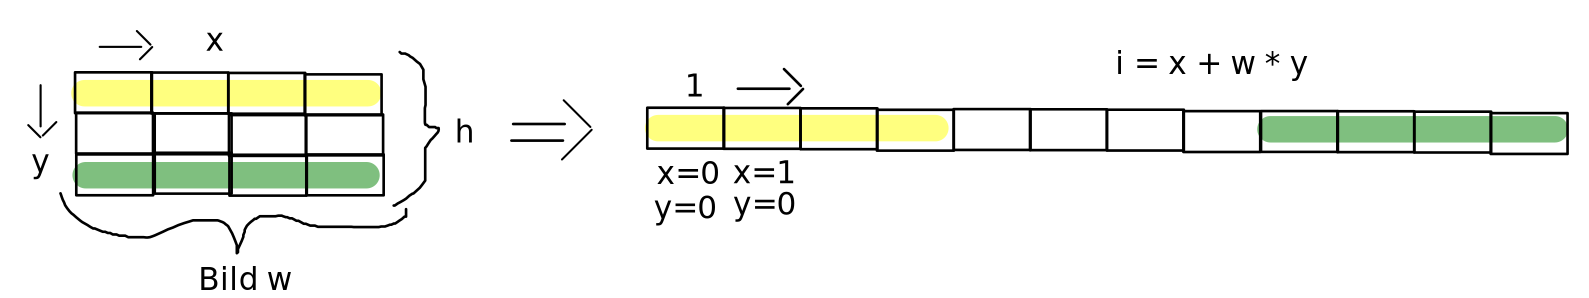
\includegraphics[width=15cm,height=8cm,keepaspectratio]{./Pictures/2D1D.png}
        \begin{minted}{python}
        for y in range(h):
            for x in range(w):
                data[x+w*y] = 0 #Initialisierung
        #Optimierung:
        for y in range(h):
            wy = w * y
            for x in range(w):
                data[x+wy]=0
        \end{minted}
        Faustregel: \glqq Vereinfachung der inneren Schleife\grqq  (wird am meisten ausgeführt)\\
        Ausnutzen der Hardware:
        \begin{itemize}
            \item Prozessor Cache: Kommunikation zwischen CPU und RAM ist langsam
            \begin{itemize}[label={$\Rightarrow$}]
                \item naiver Code: CPU wartet häufig auf RAM-Zugriff
                \item Cache Zugriffe sind schnell  $\Rightarrow$ sorge dafür, dass benötigte Daten bereits im Cache sind $\widehat{=}$ Daten, die im Speicher in der Nähe der bereits bearbeiteten Daten liegen \glqq cache locality\grqq
                \item strukturiere Schleifen so, dass in der inneren Schleife auf aufeinanderfolgende Daten zugegriffen wird
            \end{itemize}
            \item Prozessor Pipeline: jeder Befehl besteht aus Phasen, z.B.
        \end{itemize}
    \end{itemize}
    \begin{figure}[htbp]
        \begin{minipage}[t]{7cm}
            \vspace*{-2cm}
            \begin{enumerate}
                \item Dekodieren des Befehls
                \item Beschaffen der Inputdaten
                \item Ausführen des Befehls
                \item Abspeichern des Ergebnisses
            \end{enumerate}
        \end{minipage}
        \begin{minipage}{6cm}
        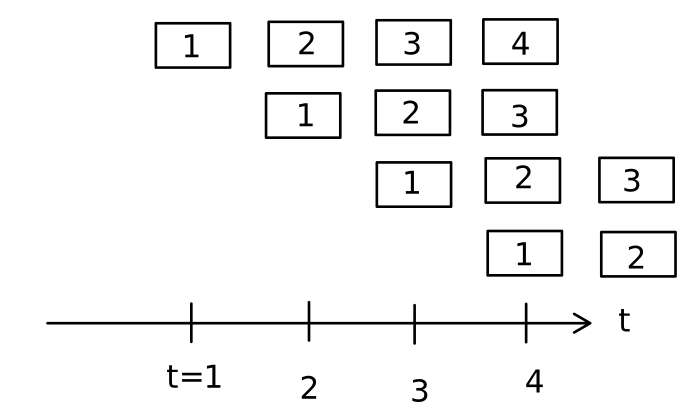
\includegraphics[width=8cm,height=5cm,keepaspectratio]{./Pictures/Pipeline.png}
        \end{minipage}
    \end{figure}
    \vspace*{-0.8cm}
    Moderne Optimierer ordnen die Befehle so um, dass die Wartezeiten minimiert werden\\
    $\underline{\text{aber}}$:
    \begin{itemize}
        \item wenn ein Befehl auf Daten wartet, müssen die Nachfolgenden auch warten
        \item if-Anweisungen: je nach Ergebnis ist der nächste Befehl anders
        \begin{itemize}[label={$\Rightarrow$}]
            \item moderne Prozessoren \glqq spekulative Ausführung\grqq
            \item komplexe if-Verschachtelungen vermeiden (auch viel lesbarer)
        \end{itemize}
        \item unnötige Typkonvertierungen vermeiden: int $\Leftrightarrow$ double
    \end{itemize}

\section*{5.2 Komplexität}
\addcontentsline{toc}{section}{5.2 Komplexität}
\begin{itemize}
    \item beschreibt den Aufwand eines Algorithmus auf abstrakter Ebene
    \item macht Algorithmen vergleichbar, unabhängig von Implementation und Hardware
\end{itemize}
\textbf{Idee:} beschreibe Anzahl der benötigten Schritte als Funktion der Problemgröße N
\begin{itemize}[label={}]
    \item $f(N)$ (kompliziert) und vereinfache sie zu einer Näherungsfunktion $g(N)$ (einfach), so dass das essentielle Verhalten von $f(N)$ und $g(N)$ gleich ist.
    \item Anschaulich: behalte dominierende Terme $\widehat{=}$ die am schnellsten wachsen
\end{itemize}
Mathematisch: Landau-Symbole, \glqq O-Notation\grqq \\
\[f(N) \in \mathcal O(g(N)) \hspace*{2cm} \mathcal O(g(N)) = \text{'Komplexitätsklasse'}\]
Definition: Es gibt ein $N_0$ (Mindestproblemgröße) und eine Konstante $c$, sodass gilt:
\[\forall N \geq N_0: f(N) \leq c g(N)\]
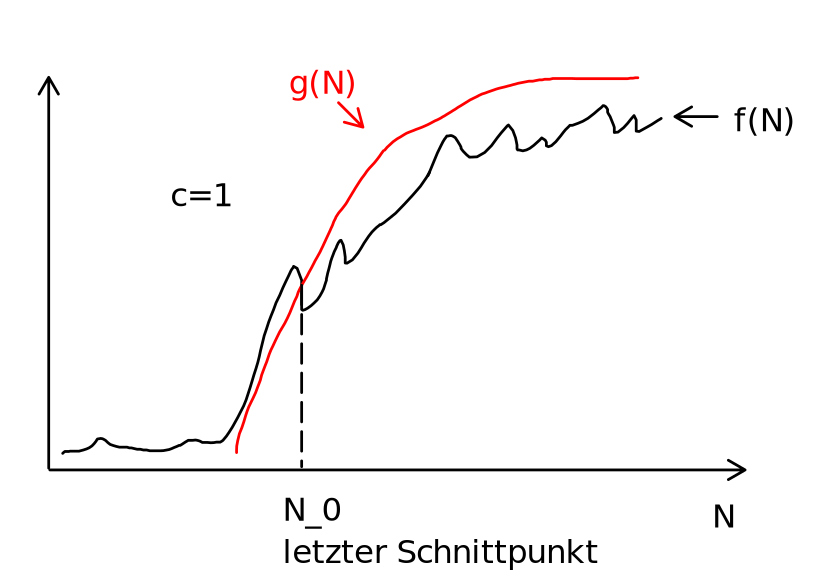
\includegraphics[width=8cm,height=5cm,keepaspectratio]{./Pictures/Komplexitaet.png}

\[\mathcal O(g(N)) := \biggl\lbrace f(N), \text{ so dass } \exists N_0, c \text{ mit } f(N) \leq c * g(N) \text{ für } N \geq N_0 \biggr\rbrace\]

Eigenschaften:
\begin{itemize}
    \item transitiv: $f(N) \in \mathcal O(g(N)) \land g(N) \in \mathcal O(h(N)) \Rightarrow f(N) \in \mathcal O(h(N))$
    \item additiv: $f(N) \in \mathcal O(h(N)) \land g(N) \in \mathcal O(h(N)) \Rightarrow f(N) + g(N) \in \mathcal O(h(N))$
    \item skalare Multiplikation: $f(N) \in \mathcal O(g(N)) \Rightarrow c* f(N) \in \mathcal O(g(N)) $
\end{itemize}

$\Rightarrow$ für Monome und Polynome gilt:
\[ x^k \in \mathcal O(x^{k+j}) \hspace*{2cm} a_0 + a_1x^1 + a_2x^2 + \dots + a_kx^k \in \mathcal O(x^k)\]
für alle $j \geq 0$ \\
Logarithmus: die Basis ist egal, d.h. $log_a(x) \in \mathcal O(log_b(x))$ für alle $a,b >1$
\[ \text{ weil  }\hspace*{1cm} log_a(x) = \frac{log_b(x)}{log_b(a)} \Rightarrow c = \frac{1}{log_b(a)}\]
Aus Multiplikation folgt auch\hspace*{1cm} $c* \mathcal O(f(N)) \in \mathcal O(f(N))$ \\
\hspace*{6cm} $\mathcal O(c*f(N)) \in \mathcal O(f(N))$ \\

mehrere $\mathcal O$'s verschwinden: $ \mathcal O( \mathcal O(f(N)) \in \mathcal O (f(N))$ \\

Spezialfall von Polynom: additive Konstanten dominieren nie \\
\hspace*{1cm}$\Rightarrow$ können weggelassen werden: $\mathcal O(f(N)) + p \in \mathcal O(f(N))$

\section*{5.3 Landau-Symbole, O-Notation}
\addcontentsline{toc}{section}{5.3 Landau-Symbole, O-Notation}
\begin{itemize}[label={}]
    \item groß-$\bigO{}$: \hspace*{5mm}$f(N)$ \glqq $\leq$\grqq $g(N)$ : $\exists N_0, c, $ so dass $\forall N \geq N_0$ gilt : $f(N) \leq c * g(N)$\\
    \hspace*{4.5cm}$\Leftrightarrow f(N) \in O(g(N))$

    \item klein-o:  \hspace*{5mm}$f(N)$ \glqq $<$\grqq $g(N) $: $\underline{\text{ für alle } c>0} : \exists N_0 $, so dass $\forall N \geq N_0$ gilt : $f(N) < c * g(N)$\\
    \hspace*{4.5cm}$\Leftrightarrow f(N) \in o(g(N))$

    \item $\Omega$:  \hspace*{5mm}$f(N)$ \glqq $\geq$\grqq $g(N)$ : $\exists N_0, c, $ so dass $\forall N \geq N_0$ gilt : $c *f(N) \geq  g(N)$\\
    \hspace*{4.5cm}$\Leftrightarrow f(N) \in \Omega (g(N))$

    \item $\omega$:  \hspace*{5mm}$f(N)$ \glqq $>$\grqq $g(N)$ : für alle $\infty > c > 0:$ $\exists N_0, $ so dass $\forall N \geq N_0$ gilt : $c* f(N) > g(N)$\\
    \hspace*{4.5cm}$\Leftrightarrow f(N) \in \omega (g(N))$

    \item $\Theta$:  \hspace*{5mm}$f(N)$ \glqq $=$\grqq $g(N)$ : $\exists N_0, c_1, c_2, $ so dass $\forall N \geq N_0$ gilt : $c_1 * g(N) \leq f(N) \leq c_2 * g(N) $\\
    \hspace*{4.5cm}$\Leftrightarrow f(N) \in \Theta (g(N))$ $\Leftrightarrow f(N) \in \bigO{} (g(N))$ $\land f(N) \in \Omega (g(N))$

    \item $\Rightarrow$ wenn  $f(N) \in o(g(N)) \Rightarrow f(N) \in O(g(N))$ \\
    Beispiele: $N \in o(N^2) \hspace*{0.6cm} \Rightarrow N \in O(N^2)$ \\
    \hspace*{0.65cm} aber: $N \not\in o(N) \hspace*{0.6cm} , \text{aber }N \in O(N)$\\
\end{itemize}

\subsection*{Anwendung auf Sortieren:}
Anzahl der Vergleiche bei :
\begin{itemize}
    \item insertion sort:
    \begin{itemize}
        \item typischer Fall: $V(N)= \frac{N(N-1)}{4} = \frac{N^2}{4} - \frac{N}{4} \in \bigO{}(N^2)$ \\
        \item schlechter Fall: $V(N) = \frac{N(N-1)}{2} = \frac{N^2}{2} - \frac{N}{2} \in  \bigO{}(N^2) $\\
    \end{itemize}
    \item quick sort:
    \begin{itemize}
        \item typischer Fall: $V(N) = 2(N+1) ln(N+1) \in \bigO{}(N*log N)$
        \item schlechter Fall: $V(N) = V(N) = \frac{(N+1)(N+2)}{2} \in \bigO{}(N^2) $\\
    \end{itemize}
\end{itemize}

\subsection*{Rechenregeln}
siehe vorige VL (oder Skript)

\subsection*{Regeln zur Anwendung auf Algorithmen}
\begin{itemize}
    \item Sequenzregel $\widehat{=}$ Nacheinander-Ausführung von Befehlen im Algorithmus \\
    anschauliche Bedeutung: der langsamste Befehl bestimmt die Komplexität \\
    $\begin{rcases}
    \text{Befehl 1} & \bigO{}(f(N)) \\
    \text{Befehl 2} & \bigO{}(g(N))\\ \end{rcases} \bigO{}(f(N)) + \bigO{}(g(N)) \begin{cases}
    \in \bigO{}(f(N)) & \text{ wenn } g(N) \in \bigO{}(f(N)) \\
    \in \bigO{}(g(N)) & \text{ wenn } f(N) \in \bigO{}(g(N)) \\ \end{cases}$ \\
    \hspace*{6.5cm} $\widehat{=} \text{max}(\bigO{}(f(N)), \bigO{}(g(N)))$
    \item Schachtelungsregel $\widehat{=}$ Ausführung eines Befehls (oder einer Sequenz) in einer Schleife \\
    anschauliche Bedeutung: Komplexität erhöht sich um die Anzahl der Durchläufe \\
    $\begin{rcases}
    \text{for k in range(N)}: & \bigO{}(N)\hspace*{3mm} \textcolor{blue}{\bigO{}(f(N))}\\
        \text{  Befehl} & \bigO{}(g(N)) \end{rcases}\bigO{}(N*g(N)) \hspace*{3mm} \textcolor{blue}{\bigO{}(f(N)*g(N))}$
        \item Wie berechnet man die Komplexität?
        \begin{itemize}
            \item vollständige Induktion:
            \begin{enumerate}
                \item Induktionsanfang: suche $N_0$ und $c$, so dass $f(N_0) \leq c*g(N_0)$
                \item Induktionsschritt: falls $f(N) \leq c*g(N)$ \\
                \hspace*{3cm} $\Rightarrow f(N+1) \leq c*g(N+1)$
            \end{enumerate}
            \item Grenzwertbildung $n \rightarrow \infty$ ($\widehat{=}$ alternative Definition von $\bigO{}$, o, etc.)
            \begin{itemize}[label={}]
                \item $f(N) \in \bigO{}(g(N)) \Leftrightarrow \lim\limits_{N \rightarrow \infty} \frac{f(N)}{c*g(N)} = 1$ für ein geeignetes $c \Leftrightarrow \lim\limits_{N \rightarrow \infty} \frac{f(N)}{g(N)} = c$
                \item $f(N) \in o(g(N)) \Leftrightarrow \lim\limits_{N \rightarrow \infty} \frac{f(N)}{g(N)} = 0$
            \end{itemize}
        \end{itemize}
    \end{itemize}

\textbf{Beispiel}: ist log(N) $\in \bigO{}(N)$, Grenzwertmethode:\\
\[\lim\limits_{N\rightarrow\infty} \frac{ln N}{N} = \frac{\infty}{\infty} \text{ ??} \]\\
Regel von l'Hospital: $\lim\limits_{x \rightarrow x_0} \frac{f(x)}{g(x)} = \lim\limits_{x \rightarrow x_0} \frac{f'(x)}{g'(x)}$ falls $\frac{f(x_0)}{g(x_0)}$ unbestimmt

\[f(N) = ln(N) \Rightarrow f'(N) = \frac{1}{N} \hspace*{1cm} g(N) = N \Rightarrow g'(N) = 1 \]
\[\lim_{N \rightarrow \infty} \frac{ln N}{N} = \lim_{N \rightarrow \infty} \frac{\frac{1}{N}}{1} = \lim_{N \rightarrow \infty} \frac{1}{N} =  \frac{''1''}{\infty} = 0  \]
\[ \Rightarrow ln N \in o(N) \]

\section*{5.4 Analyse von Algorithmen für den gleitenden Mittelwert}
\addcontentsline{toc}{section}{5.4 Analyse von Algorithmen für den gleitenden Mittelwert}
\begin{minted}{python}
def running_mean(a, k):             #N=len(a)
    r = [0] * len(a)                #O(N)
    if k > len(a):                  #O(1)
        raise RuntimeError("k too large")
    for j in range (k-1, len(a)):   #O(N-k+1) = O(N)
        for i in range(j-k+1, j+1): #O(k)
            r[j] += a[i]            #O(1) + O(1) + O(1) = O(1)
        r[j] /= float(k)            #O(1) + O(1) + O(1) = O(1)
    return r
\end{minted}
Schachtelung: $\bigO{}(k) * \bigO{}(1) = \bigO{}(k)$ \\
Schachtelung: $\bigO{}(N) * \bigO{}(k) = \bigO{}(N*k)$ \\
Sequenz:      $\bigO{}(N)+\bigO{}(1)+\bigO{}(N*k)+\bigO{}(1) = \bigO{}(N*k)$ \\

Verwende ungünstige Datenstruktur für a: \\
verkettete Liste: a[i] $\rightarrow$ get\_element(a,i) \hspace*{1cm} O(i)\\

\subsection*{Verkettete Liste}
für jedes Element: Node-Datenstruktur, enthält das Datenelement und einen zeiger/Referenz auf den nächsten Node \\

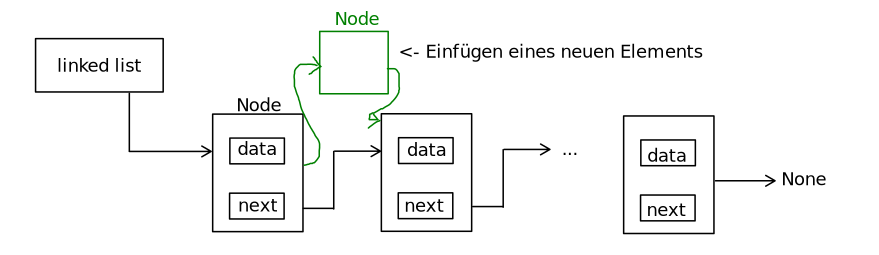
\includegraphics[width=15cm,height=9cm,keepaspectratio]{./Pictures/linkedlist.png}

Zugriff auf Element i: Durchlaufen der Kette bis Node i $\in \bigO{}(i)$ Schritte \\

Zugriff auf Element i: Durchlaufen der Kette bis Node i $\in O(i)$ Schritte \\

\textbf{Optimierte Version des gleitenden Mittels:}
\begin{minted}{python}
def running_mean_2(a, k):             #N=len(a)
    r = [0] * len(a)                  #O(N)
    if k > len(a): ...                #O(1)
    for i in range(k):                #O(k)
        r([k-1] += a[i]               #O(1) -> O(k*1)
    for j in range(k, len(a)):        #O(N)
        r[j] = r[j-1] - a[j-k] + a[j] #O(1) -> O(N)
    for j in range(k-1, len(a)):      #O(N)
        r[j] /= float(k)              #O(1) -> O(N)
    return r                          #Sequenz: maximum-> O(N) (statt O(N*k))
\end{minted}

Rechenregel: $a_0 + a_1 * N + a_2 * N^2 + \cdots + a_k * N^k \in \bigO{}(N^k)$ \\
    \hspace*{3cm} $\bigO{}(N-k) = \bigO{}(N)$


\section*{5.5 Amortisierte Komplexität}
\addcontentsline{toc}{section}{5.5 Amortisierte Komplexität}
\begin{itemize}
    \item falls dieselbe Operation manchmal schnell und manchmal langsam ist:
    \begin{itemize}
        \item wie ist das Verhalten im Mittel?
        \item Verteilt (\glqq amortisiert \grqq) sich der Aufwand von wenigen langsamen Aufrufen über viele schnelle Aufrufe?
    \end{itemize}
\end{itemize}
Anwendung: \textbf{dynamisches Array}
\begin{itemize}
    \item \textbf{Problem}: Einfügung neuer Elemente in ein statisches Array teuer: \\
    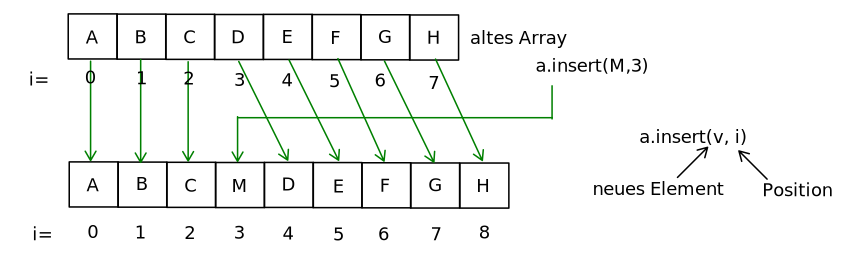
\includegraphics[width=12cm,height=9cm,keepaspectratio]{./Pictures/dynamischesArray.png}
    \begin{enumerate}
        \item neues Array mit einer zusätzlichen Speicherstelle allozieren
        \item die alten Daten kopieren $\Rightarrow \bigO{}(N)$ teuer!
        \item das neue Element einfügen
    \end{enumerate}
    \item \textbf{Lösung}: oft genügt es, wenn neue Elemente immer am Ende angehängt werden
    \item \textbf{Trick}: man alloziert \textbf{mehr} Speicher als man aktuell benötigt (z.B. 2x)
    \item \textbf{Fall 1}: Array hat noch unbenutzten Speicher: \\
    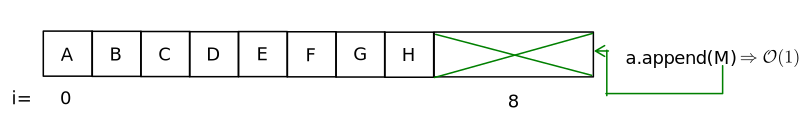
\includegraphics[width=12cm,height=9cm,keepaspectratio]{./Pictures/dynArrunbenutzt.png}
    \item \textbf{Fall 2}: Array ist voll $\Rightarrow$ kopiere in ein neues Array mit \textbf{doppelter} Größe \\
    (nicht: in ein neues Array mit einem zusätzlichen Element, wie in Beispiel 1) \\
    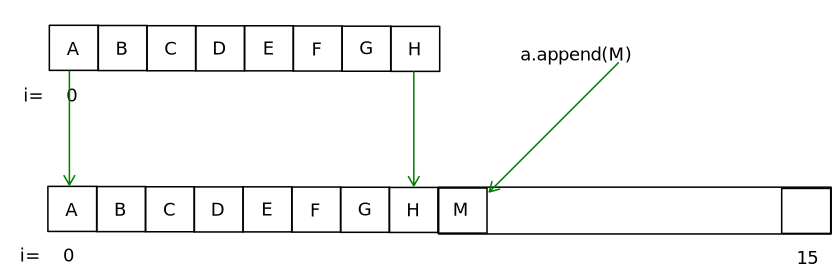
\includegraphics[width=12cm,height=9cm,keepaspectratio]{./Pictures/dynArrDopp.png}
    \begin{enumerate}
        \item alloziere Array der doppelten Größe
        \item kopiere die alten Daten \hspace*{3cm} \textcolor{blue}{$\bigO{}(N)$}
        \item kopiere neues Element  \hspace*{3.1cm} \textcolor{blue}{$\bigO{}(1)$} \\
        $\Rightarrow$ \textcolor{blue}{$\bigO{}(N)$}
    \end{enumerate}
    $\Rightarrow$ jetzt sind noch N-1 Speicherstellen frei (N-1 $\widehat{=}$ alte Arraygröße) \\
    $\Rightarrow$ jetzt bekommen wir (N-1)-mal Fall 1 mot $\bigO{}(1)$
    $\Rightarrow$ selten $\bigO{}(N)$, häufig $\bigO{}(1)$$\Rightarrow$ Was bedeutet das im Durchschnitt?

    \item Was ist die amortisierte Komplexität des \glqq Verdopplungs-Trick\grqq ?
    \item Accounting-Methode: definieren \glqq Guthaben\grqq, das wir während des billigen Anfügens ansparen und bei teuren Operationen verbrauchen \\
    $\varphi_i = \text{size}_i - \text{capacity}_i \leq 0$ weil size $\in$ capacity
\end{itemize}

Kosten einer Einfügung $c_i = \tilde{c_i} + \varphi_i - \varphi_{i-1}$\\
\begin{itemize}
    \item $c_i$ $\rightarrow$ tatsächliche Kosten der Einfügung
    \item $ \varphi_i - \varphi_{i-1}$ $\rightarrow$ verbrauchtes Guthaben
\end{itemize}

\begin{itemize}
    \item \textbf{Fall 1:} vor der i-ten Einfügung gilt size$_{i-1} < \text{capacity}_{i-1} \Rightarrow$ noch Platz
    \begin{itemize}[label={$\Rightarrow$}]
        \item $\tilde{c_i} = 1$ für das Kopieren des neuen Elements, capacity$_i = \text{capacity}_{i-1}$
    \end{itemize}
    $c_i = 1 + (\underbrace{\text{size}_i}_{\text{size}_{i-1}+1}- \text{capacity}_i) - (\text{size}_{i-1} - \text{capacity}_{i-1}) = 2$

    \item \textbf{Fall 2:} vor der i-ten Einfügung gilt: $\text{size}_{i-1} = \text{capacity}_{i-1} \Rightarrow $ Array voll \\
    \hspace*{7.8cm}  $\text{capacity}_{i} = 2*\text{capacity}_{i-1} $ \\
    \begin{itemize}[label={$\Rightarrow$}]
        \item   $\tilde{c_i} = \hspace*{-2.3cm}\underbrace{\text{size}_{i-1}}_{\text{alte Elemente in den neuen Speicher kopieren}}\hspace*{-2.3cm}+  1 \leftarrow$ neues Element kopieren
    \end{itemize}
    $c_i = \text{size}_{i-1} + 1 + (\underbrace{\text{size}_{i}}_{\text{size}_{i-1}+1} - \hspace*{-0.3cm} \underbrace{\text{capacity}_{i}}_{2*\text{capacity}_{i-1} = 2* \text{size}_{i-1}}\hspace*{-0.5cm}) - (\text{size}_{i-1} -\underbrace{ \text{capacity}_{i-1}}_{\text{size}_{i-1}}) = 2$ \\

    in beiden Fällen: $c_i = 2 \Rightarrow$ amortisierte Komplexität $\bigO{}(1)$
\end{itemize}

\begin{tabular}{l | C{0.5cm} C{1.5cm} | C{2cm} | C{1.5cm} | C{2.6cm}| C{1cm} | C{1.5cm}}
    Array & size & capacity & aktuelle Kosten $\tilde{c_i}$ & totale Kosten &  Durchschnitts- kosten & $\varphi_i$  & $c_i = \tilde{c_i} + \varphi_i - \varphi_{i-1}$\\\hline
    \mintinline{python}{[None]} & 0 & 1 & & & & -1 & \\
    \mintinline{python}{[a]} & 1 & 1 & 1 & 1 & 1 & 0 & 2\\
    \mintinline{python}{[a,b]} & 2 & 2 & 1+1 & 3 & 3/2 & 0 & 2\\
    \mintinline{python}{[a,b,c, None]} & 3 & 4 & 2+1 & 6 & 6/3 & -1 & 2\\
    \mintinline{python}{[a,b,c,d]} & 4 & 4 & 0+1 & 7 & 7/4 & 0 & 2\\
    \mintinline{python}{[a,b,c,d,e,None,None,None]} & 5 & 8 & 4+1 & 12 & 12/5 & -3 & 2 \\
    \mintinline{python}{[a,b,c,d,e,f,None,None]} & & & & &&-2 & 2\\
    \mintinline{python}{[a,b,c,d,e,f,g,None]} & & & & && -1 & 2\\

\end{tabular}




\chapter{Suchen}
Viele Arten von Suchen:
\begin{itemize}
    \item \textbf{Schlüsselsuche}: suche Elemente, deren Schlüssel einem vorgegebenen Schlüssel entspricht
    \item Bereichssuche: ein Intervall von gültigen Werten wird gesucht
    \item Nachbarschaftssuche / Ähnlichkeitssuche: Elemente, die einem gegebenen Element ähnlich sind (z.B. Internetsuche)
    \item $\underline{\text{Graphensuche}}$: suche einen Weg von einem gegebenen Knoten zu einem anderen (z.B. Navigationsprogramm)
\end{itemize}

\section{Schlüsselsuche}

\subsection*{naive Methode: sequentielle Suche}
Vorbedingungen:
\begin{itemize}
    \item Daten liegen in einem Array
    \item Datenelemente können auf Identität (==) des Schlüssels verglichen werden
\end{itemize}

\begin{minted}{python}
def sequential_search(a, target_key, key_func):
    for i in range(len(a)):
        if key_func(a[i]) == target_key:
            return i        # gefunden bei Index i
    return None             # nichts gefunden
                            # oder "return -1"
    \end{minted}

    Vereinfachung: die Datenelemente sind der Schlüssel

    \begin{minted}{python}
def sequential_search(a, target_key):   #Komplexitaet:
    for i in range(len(a)):             #O(N)
        if a[i] == target_key:          #O(1)
            return i
    return None                         #O(1)
        \end{minted}
        \begin{itemize}
            \item Fall 1: nichts gefunden: $\bigO{}(N) * \bigO{}(1) + \bigO{}(1) = \bigO{}(N)$
            \item Fall 2: gefunden: im Schnitt: $\frac{N}{2}$ Schritte $\Rightarrow \bigO{}(N)$
        \end{itemize}
        $\Rightarrow$ \glqq lineare Suche\grqq

        \subsection*{Schnellere Suche: binäre Suche}
        Vorbedingungen:
        \begin{itemize}
            \item Elemente sind in sortiertem Array
            \item auf den Elementen gibt es eine totale Ordnung \\
            $\Rightarrow$ impliziert Identität: a==b $\Leftrightarrow$ not(a$<$b) and not (b$<$a)
        \end{itemize}

        $\Rightarrow$ Suche nach devide-and-conquer Prinzip\\
        \begin{minted}{python}

 a = [...]
 a.sort()
 found = binary_search(a, target_key)

 def binary_search(a, target_key):
     return binary_search_impl(a, target_key, O, len(a))

 def binary_search_impl(a, target_key, start, end):
     size = end - start
     if size <= 0:
         return None                    # nichts gefunden
     center = (start+end) // 2          # floor-Division
     if a[center] == target_key:
         return center                  # gefunden bei Index center
     elif a[center] < target_key:
         return binary_search_impl(a, target_key, center+1, end)
     else:
         return binary_search_impl(a, target_key, start, center)
        \end{minted}

        \subsection*{Komplexität der binären Suche}

        \begin{itemize}
            \item vorab: Sortieren O(N log N)
            \item Alg. selbst: V(N) = 2 + V(N/2) = 2 + 2 + V(N/4) = ...\\
            \hspace*{3cm} = $\underbrace{ 2 + 2 + ... + 2}_{[ log_2(N)] \text{Summanden}} = 2* \lceil log_2 (N) \rceil = O(logN)$
        \end{itemize}
        \begin{itemize}[label={$\Rightarrow$}]
            \item wesentlich schneller als sequentielle Suche, \textbf{aber} man muss vorab sortieren
            \item Sortieraufwand amortisiert sich über viele Suchanfragen, wenn man mindestens $\Omega(log N)$ Suchen ausführt
        \end{itemize}

        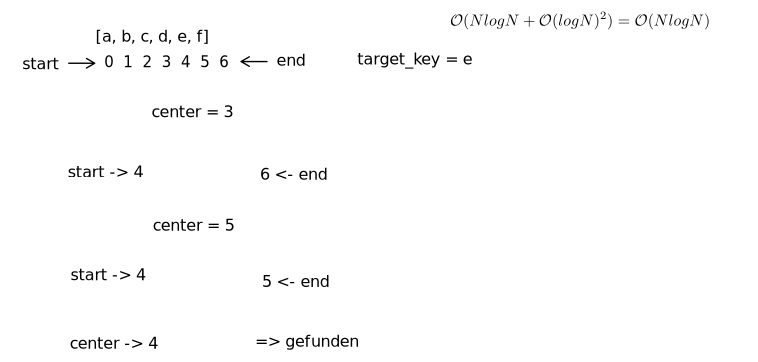
\includegraphics[width=12cm,height=9cm,keepaspectratio]{./Pictures/binaereSuche.png}

        Anwendung: Daten werden vorab gesammelt und ändern sich dann nicht mehr\\
        $\Rightarrow$ einmal sortieren, viele Suchvorgänge\\

        ungünstig: Datenarray ändert sich häufig (Einfügen oder Löschen von Elementen)\\
        $\Rightarrow$ Sortieraufwand amortisiert sich nicht $\Rightarrow$ Suchbäume oder Hashtabelle verwenden

        \section{Suchbäume}

        \begin{itemize}
            \item effiziente Suche, wenn der Datenbestand sich häufig ändert
            \item \glqq Bäume mit Wurzel\grqq = rooted trees \\
            \begin{itemize}
                \item spezielle Graphen, wo es von jedem Knoten zu jedem anderen genau einen Weg gibt
                \item ein ausgezeichneter Knoten heißt \glqq Wurzel\grqq , die zeichnet man oben :-)\\
                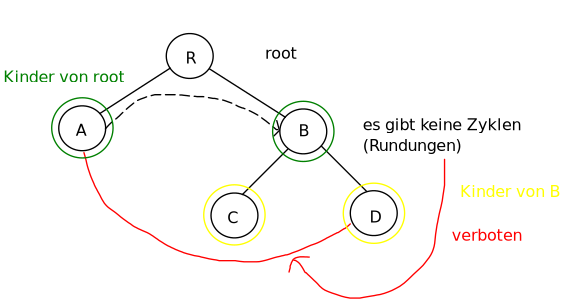
\includegraphics[width=9cm,height=7cm,keepaspectratio]{./Pictures/binaerBaum.png}
                \item speziell: Binärbäume – jeder Knoten hat maximal zwei Kinder
                \item Kinder sind Nachbarknoten, die weiter von der Wurzel entfernt sind
            \end{itemize}
            in Python: Hilfsklasse für Knoten, die ein Datenelement und maximal 2 Kinder speichert

\begin{minted}{python}
class Node:
    def __init__(self, key):
        self.key = key
        self.left = self.right = None       #anfangs keine Kinder
root = Node("R")
root.left = Node("H"); root.right = Node("B"); root.right.left = Node("C")
\end{minted}
        \end{itemize}

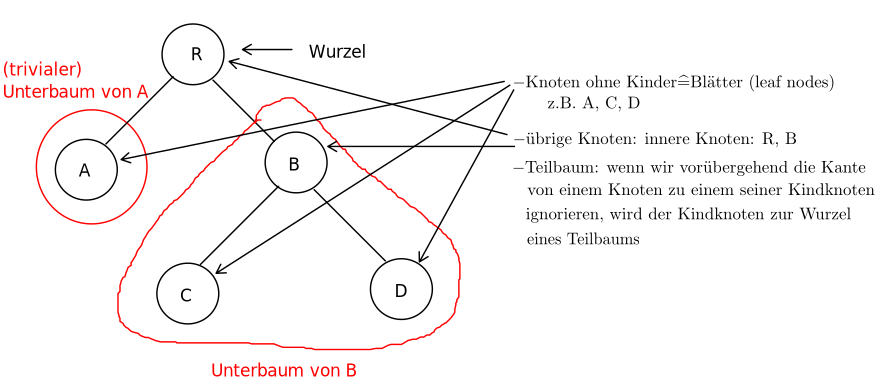
\includegraphics[width=13cm,height=10cm,keepaspectratio]{./Pictures/binaerBaum2.png}

\textbf{Suchbaum}:
\begin{enumerate}
    \item auf den Schlüsseln ist eine Ordnung definiert \glqq $<$\grqq (wie Sortieren)
    \item für jeden Knoten gilt:
    \begin{enumerate}[label=\alph*)]
        \item die Schlüssel im linken Teilbaum sind alle kleiner als der Schlüssel des Knotens
        \item die Schlüsse im rechten Teilbaum sind alle größer als der Schlüssel des Knotens
    \end{enumerate}
    (vgl.: analoges Verhalten beim Pivot in quick sort)
\end{enumerate}
\begin{itemize}
    \item zur Erinnerung: \\
    \begin{minted}{python}
class Node:
    def __init__(self, key):    #bei echten Anw: , data)
        self.key = key
        self.left = self.right = None
    \end{minted}
    \item Idee der Suche:
    \begin{itemize}
        \item wenn der Schlüssel gefunden: gib den betreffenden Node zurück
        \item sonst suche im linken oder rechten Teilbaum weiter $\Rightarrow$ \glqq teile und herrsche\grqq
        \item wenn ein Blatt und key nicht gefunden: gib None zurück
    \end{itemize}
\end{itemize}

\begin{minted}{python}
def tree_search(node, key):
    if node is None:                        # nichts gefunden, Rekursionsabschluss 1
        return None
    if key == node.key:                     # gefunden! Rekursionsabschluss 2
        return node
    if key < node.key:
        return tree_search(node.left, key)  # links weitersuchen
    else:
        return tree_search(node.right, key) # rechts weitersuchen
\end{minted}

Verwendung:
\begin{itemize}[label ={}]
    \item root = ...    \hspace*{1cm} \#Wurzel des Suchbaums
    \item result = tree\_search(root, key)
\end{itemize}
$[$ in einer Programmbibliothek würde man all das noch \glqq kapseln\grqq , so dass der Nutzer nur ein interface sieht, aber nicht die interne Funktionalität, z.B. Klasse Node $]$ \\

\textbf{Einen neuen Schlüssel in den Baum einfügen}
\begin{itemize}
    \item muss auch funktionieren, wenn Baum leer $\widehat{=}$ root = None
    \item muss auch funktionieren, wenn der Schlüssel schon vorhanden ist \\
    Möglichkeiten:
    \begin{itemize}
        \item Fehlermeldung (Exception)
        \item besser: nur die mit dem Schlüssel verknüpften Daten überschreiben \verb|a["Fritz Mueller"] = 1.0|
    \end{itemize}
\end{itemize}

\begin{minted}{python}
def tree_insert(node, key):                         # in der Praxis: ,data)
    if node is None:                                # richtigen Platz gefunden
        return Node(key)                            # Konstruktor
    if key == node.key:                             # Schluessel schon vorhanden
        return node                                 # in Praxis: Daten ersetzen vorher
    if key < node.key:                              # key gehoert in den linken Teilbaum
        node.left = tree_insert(node.left, key)     #Rekursion
    else:
        node.right = tree_insert(node.right, key)   #Rekursion
    return node
\end{minted}

Verwendung:
\begin{minted}{python}
root = None                     # leerer Baum
root = tree_insert(root, 4)
root = tree_insert(root, 2)
root = tree_insert(root, 3)
root = tree_insert(root, 6)
\end{minted}

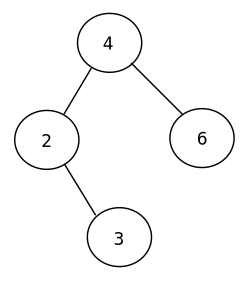
\includegraphics[width=4cm,height=4cm,keepaspectratio]{./Pictures/zahlenbaum.png}

Wenn die Schlüssel in ungünstiger Reihenfolge eingefügt werden (z.B. sortiert oder umgekehrt sortiert), erhält man statt eines Baums eine Kette ($\widehat{=}$ verkettete Liste) mit sehr langsamem Suchverhalten \\

Einfügen in der Reihenfolge 1, 2, 3, 4, 5 \\

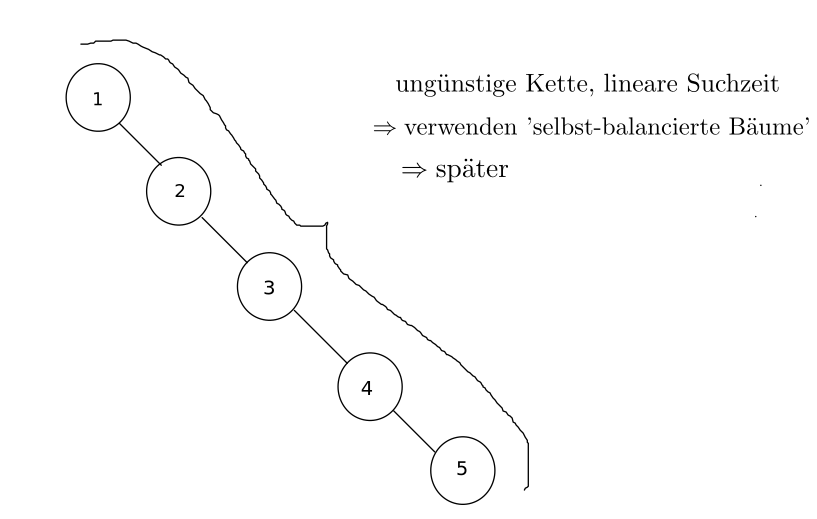
\includegraphics[width=12cm,height=7cm,keepaspectratio]{./Pictures/Kette.png}

\textbf{Entfernen eines Schlüssels aus dem Baum}\\
vier Fälle:
\begin{enumerate}
    \item der Schlüssel ist nicht vorhanden:
    \begin{itemize}
        \item Fehlermeldung
        \item remove gibt None zurück $\widehat{=}$ nichts entfernt
    \end{itemize}
    \item Schlüssel ist in einem Blatt $\Rightarrow$ kann ihn einfach entfernen
    \item Schlüsselknoten hat ein Kind $\Rightarrow$ kann ihn durch Teilbaum des Kindes ersetzen
    \item Schlüsselknoten hat zwei Kinder $\Rightarrow$ ersetze nur den Schlüssel (plus evtl. die Daten) durch den Schlüssel eines geeigneten Blatts ($\rightarrow$ der Vorgänger des zu entfernenden Schlüssels)  und entferne dann dieses Blatt
\end{enumerate}

\begin{minted}{python}
def tree_predecessor(node):
    node = node.left                # suche größten Key im linken Teilbaum
    while node.right is not None:
        node = node.right
    return node

def tree_remove(node, key):
    if node is None:  # nicht gefunden
        return None
    if key < node.key:
        node.left = tree_remove(node.left, key)
    elif key > node.key:
        node.right = tree_remove(node.right, key)
    else:  # key gefunden
        if node.left is None and node.right is None:  #Blatt
            node = None
        elif node.left is None:  # node hat nur ein Kind
            node = node.right
        elif node.right is None:  # node hat nur ein Kind
            node = node.left
        else:  # node hat 2 Kinder
            pred = tree_predecessor(node)
            node.key = pred.key  # recycle node fuer seinen Vorgaenger
            node.left = tree_remove(node.left, pred.key)
    return node
\end{minted}

Verwendung: \verb|root = tree_remove(root, key)|

%irgendwo fehlt noch die Komplexität

\subsection*{Komplexitätsanalyse der Suchbaumfunktion (ungünstiger Fall)}
zwei Möglichkeiten:
\begin{itemize}
    \item key gefunden
    \item stelle fest, dass key nicht vorhanden
\end{itemize}
intuitiv: wenn Entscheidung viele Vergleiche erfordert $\Rightarrow$ langsam \\
\textbf{Begriffe:}
\begin{itemize}
    \item \textbf{Pfade}: Folge von Knoten $n_1, n_2, \cdots, n_k$ \\
    so dass:
    \begin{itemize}
        \item $n_i$ und $n_{i-1}$ sind Nachbarn
        \item $n_1, n_n$ sind zwei Knoten, zwischen denen wir den Pfad suchen
    \end{itemize}
    \item \textbf{Länge des Pfades}: Anzahl der Kanten, k-1
    \item \textbf{Tiefe eines Knotens im Baum}: Länge des Pfades bis root
    \item \textbf{Tiefe des Baums}: maximale Tiefe eines Knotens
\end{itemize}
$\Rightarrow$ ungünstiger Fall: key wird am Ende des längsten Pfades gefunden bzw. nicht-vorhandensein festgestellt

\begin{figure}[htbp]
    \begin{minipage}[t]{6cm}
        \vspace{0pt}
        \begin{itemize}
            \item \textbf{Balance eines Baumes}: die Pfade von der Wurzel zum \glqq Entscheiden\grqq sollten möglichst ähnliche Länge haben
            \item \textbf{Trick}: zusätzlicher \emph{virtueller} Knoten $\widehat{=}$ \textbf{Sentinel}\\
            darauf zeigen alle Knoten, die den Wert None (als linkes oder rechtes Kind) speichern\\
            in Python: das None-Objekt
        \end{itemize}
        $\Rightarrow$ RS-Pfade: von root zum Sentinel
    \end{minipage}
    \begin{minipage}[t]{6cm}
        \vspace{-1cm}
        \centering
        \hspace*{2cm} 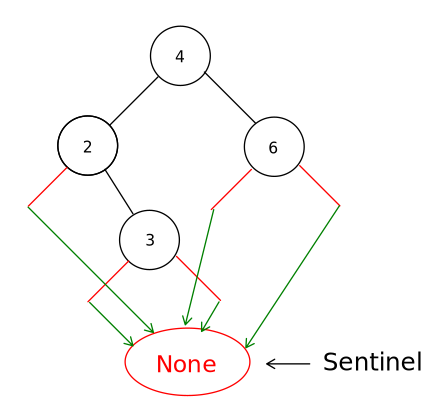
\includegraphics[width=8cm,height=8cm,keepaspectratio]{./Pictures/Sentinel.png}
    \end{minipage}
\end{figure}

\subsection{Balance des Baumes:}
Differenz zwischen kürzestem und längstem RS-Pfad

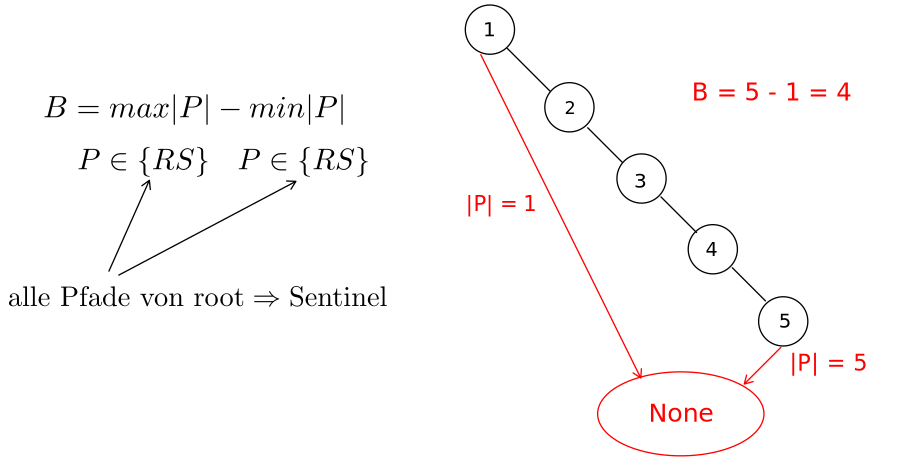
\includegraphics[width=15cm,height=5cm,keepaspectratio]{./Pictures/Kettenbalance.png}

\subsubsection{Vollständiger Baum:}
B = 0 $\rightarrow$ alle Knoten haben entweder 2 oder 0 Kinder

\begin{figure}[htbp]
    \begin{minipage}[t]{8cm}
        \vspace{0pt}
            \centering
             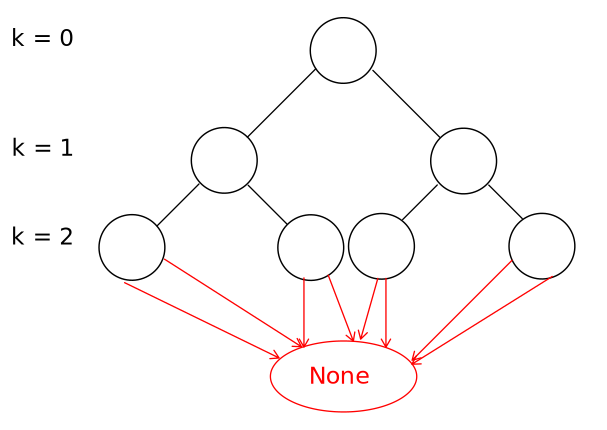
\includegraphics[width=8cm,height=4cm,keepaspectratio]{./Pictures/vollstBaum.png}
    \end{minipage}
    \begin{minipage}[t]{6cm}
        \vspace{1cm}
        Anzahl der Knoten im vollständigen Baum: bei Tiefe $k$ gibt es immer $2^k$ Blätter \\
        \hspace*{1cm} $N = 2^0 + 2^1 + \cdots + 2^{D+1} -1$ \\
        \hspace*{1cm} $D \widehat{=}$ Tiefe
    \end{minipage}
\end{figure}

\subsubsection{Perfekt balancierter Baum}
B $\leq$ 1 \\
$\Rightarrow$ für jeden Knoten gilt:
\begin{figure}[htbp]
    \begin{minipage}[t]{8cm}
        \vspace{0pt}
        \centering
        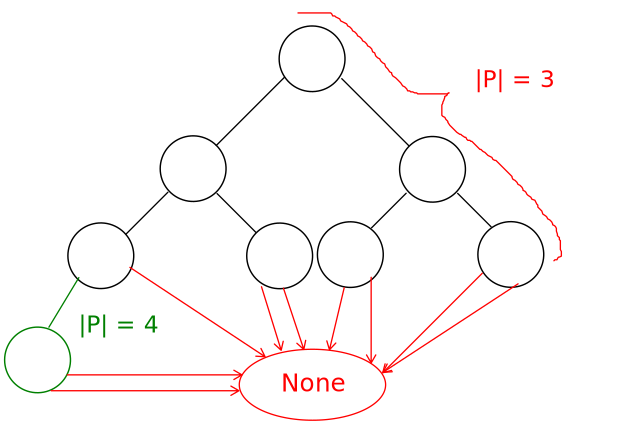
\includegraphics[width=8cm,height=5cm,keepaspectratio]{./Pictures/perfektbalanBaum.png}
    \end{minipage}
    \begin{minipage}[t]{6cm}
        \vspace{1cm}
        \begin{itemize}
            \item linker und rechter Unterbaum sind auch perfekt balanciert
            \item Tiefen von linkem und rechtem Unterbaum unterscheiden sich höchstens um 1
        \end{itemize}
    \end{minipage}
\end{figure}

\section{Balance von Suchbäumen}
B = (längster Pfad Wurzel $\rightarrow$ Sentinel) - (kürzester Pfad Wurzel $\rightarrow$ Sentinel)

\begin{figure}[htbp]
    \begin{minipage}[t]{8cm}
        \vspace{0pt}
        \centering
        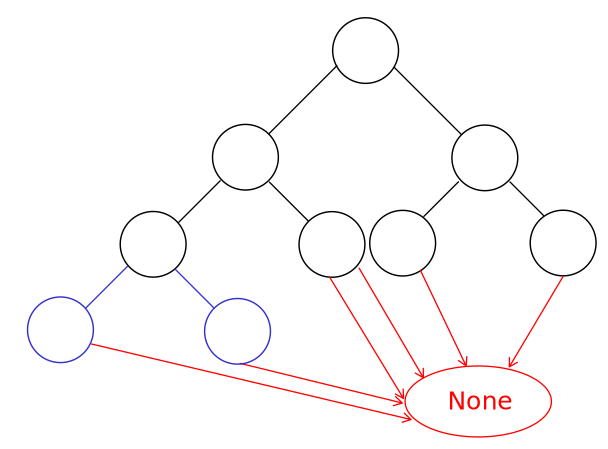
\includegraphics[width=8cm,height=5cm,keepaspectratio]{./Pictures/BalanBaum.png}
    \end{minipage}
    \begin{minipage}[t]{6cm}
        \vspace{1cm}
        \begin{itemize}
            \item vollständiger Baum, Tiefe 2
            \item \textcolor{blue}{perfekt balancierter Baum der Tiefe 3, d.h. B $\leq$ 1}
        \end{itemize}
    \end{minipage}
\end{figure}

Wieviele Elemente hat ein perfekt balancierter Baum der Tiefe $d$?
\begin{itemize}
    \item für Tiefe $d$ muss es mindestens ein Element mit Abstand $d$ von der Wurzel geben \\
    $\Rightarrow$ mindestens ein Element mehr als der vollständige Baum der Tiefe ($d$-1): $N_v = 2^d -1$\\
    $N_p \geq 2^d$
    \item um in die Tiefe $d$ zu passen, darf der perfekt balancierte Baum höchstens ein vollständiger Baum sein $\Rightarrow$ $N_p \leq 2^{d+1} -1$
\end{itemize}
\begin{itemize}[label={$\Rightarrow$}]
    \item Komplexität der Suchoperationen: Anzahl der Vergleiche $\widehat{=}$ Länge des längsten RS-Pfades im ungünstigsten Fall, \textcolor{red}{$V \in \bigO{}(d)$} beim perfekt balancierten Baum der Tiefe $d$ \\
    \[ 2^d \leq N_p \leq 2^{d+1} - 1 \hspace*{2cm} log_2(2^d) \leq log_2(N_p) \leq log_2(2^{d+1}-1) < log_2(2^{d+1})\]
    \item $d\leq log_2(N_p) < d + 1 \Rightarrow$ \textcolor{red}{$V \in \bigO{}(d) \Leftrightarrow \bigO{}(log N_p)$}\\
    \textcolor{red}{wie bei binärer Suche, also schnell.}
    \item Folgerung:
\end{itemize}wenn Baumoperationen schnell sein sollen, müssen wie sicherstellen, dass der Baum balanciert ist $\Rightarrow$ nach jedem insert oder remove wird die Balance \glqq repariert\grqq

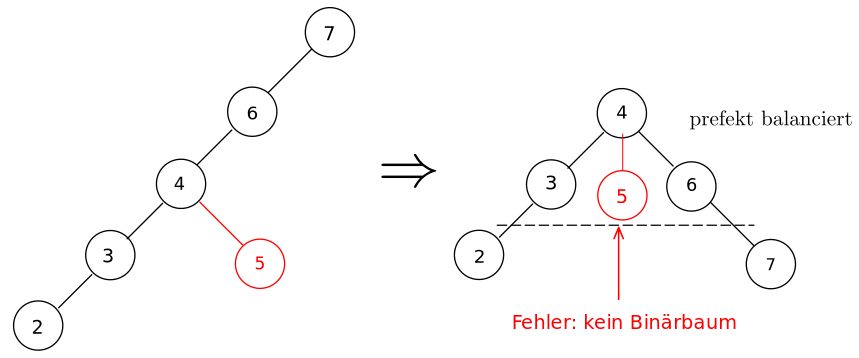
\includegraphics[width=15cm,height=5cm,keepaspectratio]{./Pictures/Reparatur.png}

3 Regeln für die Reparatur:
\begin{enumerate}
    \item Der Baum muss ein Binärbaum bleiben
    \item Die Suchbaumbedingung muss weiter gelten
    \item Die Reparatur soll lokal erfolgen (in der Nähe des aktuellen Knotens) $\Rightarrow$ Effizienz
\end{enumerate}

Grundlegende Operation: \textbf{Baumrotation}: ändert die Wurzel eines Teilbaums nach obigen Regeln, so dass Balance besser wird

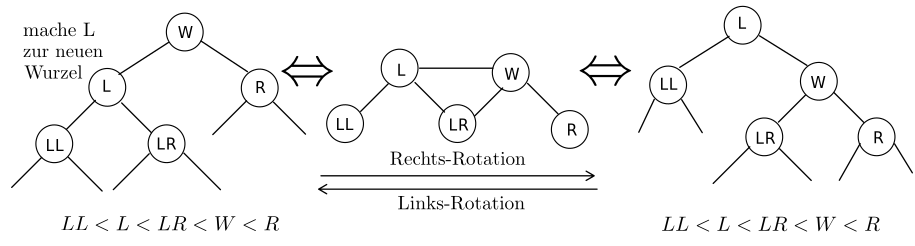
\includegraphics[width=16cm,height=6cm,keepaspectratio]{./Pictures/Rotation.png}

in Python:
\begin{minted}{python}
def tree_rotate_right(node):
    new_root = node.left
    node.left = new_root.right
    new_root.right = node
    return new_root
\end{minted}

\begin{minted}{python}
def tree_rotate_left(node):
    new_root = node.right
    node.right = new_root.left
    new_root.left = node
    return new_root
\end{minted}

Beispiel: AVL-Bäume
\begin{itemize}
    \item transformieren den Baum immer in perfekte Balance
    \item aber: das ist schwierig und unnötig,
\end{itemize}
\begin{itemize}[label={$\Rightarrow$}]
    \item \glqq einfache\grqq Balance reicht aus: \[ V \in \bigO{}(d)\]
    \[ V \leq c - d \text{ für geeignete Konstante (unabhängig von d bzw. N)}\]
    \item wenn die Tiefe nur um einen konstanten Faktor schlechter ist als beim perfekt balancierten Baum, verschwindet die Konstante in $\bigO{}(d)$ $\Rightarrow$ gleiche Komplexität
    \item viel einfachere Implementation \\
    Beispiele:
    \begin{itemize}
        \item Rot-Schwarz-Baum (typische Implementation)
        \item Treap ($\Rightarrow$ siehe Hausaufgabe)
        \item Anderson-Baum (Vereinfachung des Rot-Schwarz-Baum)
    \end{itemize}
\end{itemize}

\section{Anderson-Bäume}
Idee: jeder Knoten hat ein \emph{level} $\widehat{=}$ Abstand (kürzester Pfad) zum None-Sentinel

\begin{minted}{python}
class AndersonNode:
    def __init__(self, key):
        self.key = key
        self.left = self.right = None
        self.level = 1  #distance to None in left and right
\end{minted}

Idee: Im Anderson-Baum gibt es
\begin{itemize}
    \item horizontale Kanten (parent.level == child.level)
    \item vertikale Kanten (parent.level == child.level + 1)
\end{itemize}
\textbf{Regeln:}
\begin{itemize}
    \item die reduzierte Länge eines Pfades r: nur die vertikalen Kanten gezählt
    \item Sentinel hat level == 0 und alle Kanten zum Sentinel sind vertikal \\
    $\Rightarrow$ echte Knoten haben level $\geq$ 1
    \item reduzierte Höhe ($h_r$)  eines Knotens entspricht der reduzierten Pfadlänge ($r$)
    \item Alle RS-Pfade haben die \textbf{gleiche} reduzierte Länge. $\Rightarrow$ jeder Knoten, insbesondere die Wurzel werden auf allen Pfaden von None nach der gleichen Anzahl vertikaler Kanten erreicht (\emph{aber}: die Anzahl horizontaler Kanten kann verschieden sein)
    \item kein Pfad darf zwei horizontale Kanten hintereinander haben
    \item Vereinfachung durch Anderson: nur Kanten zum rechten Kind dürfen horizontal sein (sonst: Rot-Schwarz-Baum)
\end{itemize}
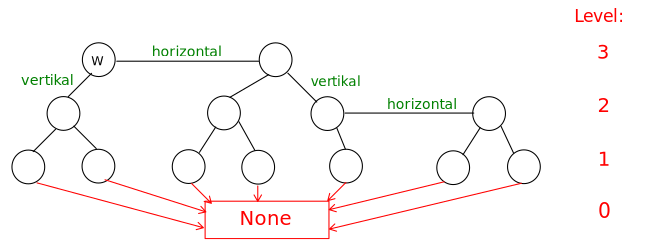
\includegraphics[width=16cm,height=4.5cm,keepaspectratio]{./Pictures/Anderson.png}

\textbf{Satz:} jeder Anderson-Baum ist balanciert (höchstens einen konstanten Faktor schlechter als der perfekt balancierte Baum), Beweis:
\begin{enumerate}
    \item $h_r$ = reduzierte Höhe des Baums (Abstand Wurzel $\rightarrow$ Sentinel \emph{ohne} horizontale Kanten)
    \begin{itemize}
        \item hat der Baum \emph{keine} horizontalen Kanten $\Rightarrow$ vollständiger Baum Tiefe $d_v = h_r - 1$
        \item hat der Baum horizontale Kanten, hat er \emph{mehr} Konten als der vollständige Baum
        \[ N \geq 2^{d_v +1} - 1 = 2^{h_r}-1\]
    \end{itemize}
    \item Da nie zwei horizontale Linien aufeinander folgen, ist die tatsächliche Tiefe höchstens zweimal die reduzierte Tiefe: $d \leq 2 * h_r$
    \item Zusammenfassen
    \[ N \geq 2^{d/2} - 1 \hspace*{2cm} N+1 \geq 2^{1/2} \]
    \[ log_2(N+1) \geq d/2 \hspace*{1.2cm} d \leq 2 log_2(N+1)) \]
\end{enumerate}
Da der schlechteste Fall des Suche: $V \in \bigO{}(d) = \bigO{}(2 log_2(N+1))$\\
\hspace*{6.45cm} $\Rightarrow \boxed{V = \bigO{}(log N)}$ \hspace*{5cm} $\square$ \\

Prinzip, den Baum balanciert zu halten bei \emph{insert}:
\begin{itemize}
    \item füge den neuen Knoten normal ein (rekursive Aufrufe von \verb|tree_insert|)
    \item prüfe, ob die Anderson-Bedingungen beim parent des neuen Knotens verletzt sind $\Rightarrow$ repariere den Unterbaum von parent
    \item auf dem Rückweg der Rekursion: prüfe und repariere auch alle Vorfahren auf dem Pfad bis zur Wurzel
\end{itemize}
in Python:
\begin{minted}{python}
def anderson_tree_insert(node, key):
    if node is None:
        return AndersonNode(key)
    if key == node.key:
        #Daten aktualisieren
        return node
    if key < node.key:
        node.left = anderson_tree_insert(node.left, key)
    else:
        node.right = anderson_tree_insert(node.right, key)
    # bis hier wie bei tree_insert()
    # ab hier Balance reparieren
    if node.left is not None and node.level == node.left.level:
        node = tree_rotate_right(node)      #turn left horizontal into right horizontal
    if node.right is not None and node.right.right is not None and node.level == node.right.right.level:    #zwei horizontal hintereinander
    # node.right -> anheben und zur Wurzel machen
    node = tree_rotate_left(node)
    node.level += 1
    return node
\end{minted}
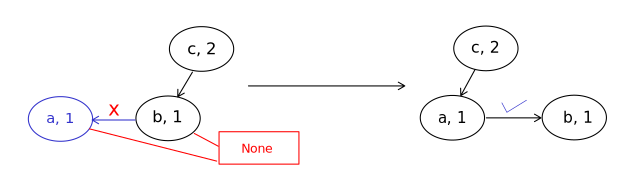
\includegraphics[width=16cm,height=3cm,keepaspectratio]{./Pictures/AndersonPython1.png}

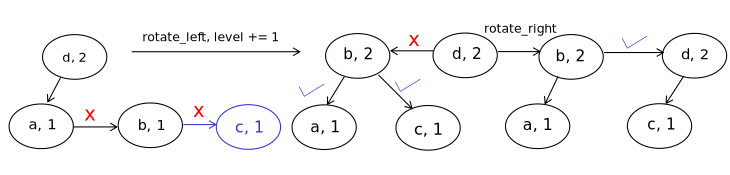
\includegraphics[width=16cm,height=3cm,keepaspectratio]{./Pictures/AndersonPython2.png}

\section{Prioritätssuche}
\begin{itemize}
    \item Variante der Suche: statt nach einem konstanten Schlüssel suchen wir den
    \begin{itemize}
        \item größten Schlüssel (max-priority search)
        \item kleinsten Schlüssel (min-priority search)
    \end{itemize}
    \item andere Interpretation als Verallgemeinerung von Stack und Queue, anschaulich: Elemente mit hoher Priorität dürfen in der Schlange vordrängeln
    \begin{itemize}
        \item Annahme: beim push in Stack oder Queue wird für das betreffende Element der Zeitstempel mitgespeichert
        \item definiere Priorität als $| now - timestamp_i| \Rightarrow$ höchste Priorität $\widehat{=}$ am längsten im Container \\
        \hspace*{1cm} $\Rightarrow$ first-come – first-served Verhalten $\widehat{=}$ Queue \\
        $\Rightarrow$ kleinste Priorität $\widehat{=}$ am kürzesten im Container $\Rightarrow \begin{rcases} \text{last-come – first-served} \\
            \text{last in - first out}\end{rcases}$ Stack
    \end{itemize}
        \item elementare Eigenschaft: max priority search $\Leftrightarrow$ zu min priority search mit negierten Schlüsseln
        \item naive Implementation: sequentielle priority search:
        \begin{minted}{python}
def sequential_priority_search(a):  #max priority
    m = 0
    for i in range(1, len(a)):
        if a[i] > a[m]:
            m = i
    return m        # Index des groessten Elements
    # => innere Schleife von selection sort (aber min priority) => O(N)
        \end{minted}
        \item Implementation mittels Suchbaum: das größte Element ist das \glqq rechteste Kind\grqq
        \begin{minted}{python}
def tree_priority_search(node):
    if node is None:
        raise KeyError("empty tree")
    while node.right is not None:
        node = node.right
    return node
    # => sehr aehnlich zu tree_predecessor (aber min pr.) => O(d) = O(log N) im balancierten Baum
        \end{minted}
        \item Beobachtung: $\bigO{}(logN)$ kann man viel einfacher erreichen als mit einem Suchbaum $\Rightarrow$ Heap (\glqq priority search tree\grqq  )
        \begin{itemize}
            \item ersetze Suchbaumbedingung durch Heapbedingung: \\
            \glqq kein Schlüssel im linken oder rechten Teilbaum hat höhere (niedrigere) Priorität als die Wurzel jedes Teilbaums im max heap (min heap)\grqq
            \item das erweist sich als viel einfacher, weil man
            \begin{enumerate}
                \item immer einen perfekt balancierten Baum garantieren kann (ohne komplexe Umstrukturierungen wie beim Andersson-Baum)
                \item den Baum als Array (= sehr effizient) speichern kann
            \end{enumerate}
        \end{itemize}
        $\Rightarrow$ linkslastigeR perfekt balancierteR Baum kann eindeutig \glqq geflattet\grqq werden, d.h. als Array \glqq flachgedrückt\grqq
        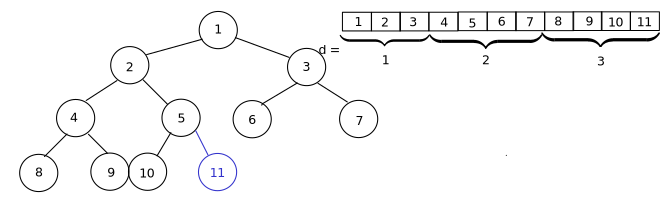
\includegraphics[width=16cm,height=4cm,keepaspectratio]{./Pictures/Flatten.png}
        \begin{itemize}
            \item Adressierung der Knoten im geflatteten Baum a \\
            \begin{itemize}
                \item a[0] $\Rightarrow$ Wurzel
                \item a[1], a[2] linkes und rechtes Kind der Wurzel
                \item a[3], a[4] linkes und rechtes Kind von a[1] usw.
                \item generell gilt:
                \begin{itemize}
                    \item die Kinder von a[i] sind a[2*i + 1] linkes Kind \\
                    \hspace*{8cm} a[2*i + 2] rechtes Kind
                    \item der Parent von a[i] ist a[(i-1) // 2] (floor division $\rightarrow$ abrunden)
                \end{itemize}
                \item die Umrechnungen ersetzen die Zugriffe \verb|node.left| und \verb|node.right| im Suchbaum
            \end{itemize}
        \end{itemize}
        \item aus der Heap-Bedingung folgt: das Element mit größter Priorität ist immer die Wurzel des ganzen Baums: a[0]
        \begin{minted}{python}
def heap_largest(a):
    return a[0]         #Komplexitaet O(1)
        \end{minted}
        \item Einfügen in den Heap: Nutze die Eigenschaft des dynamischen Arrays, das Einfügen am Ende billig ist (amortisiertes $\bigO{}(1))$:
        \begin{itemize}
            \item füge neue Elemente am Ende an (dann bleibt der Baum linkslastig perfekt balanciert)
            \item repariere eventuell die Heap-Bedingung, falls das neue Element größer als sein parent ist.
        \end{itemize}
        in Python:
        \begin{minted}{python}
def heap_insert(a, key):        #max heap
    a.append(key)               #am Ende anhaengen
    upheap(a, len(a)-1)     #reparieren des aktuell gueltigen Bereichs

def upheap(a, k):
    v = a[k]        #zwischenspeichern
    while True:     #Endlosschleife (durch "break" verlassen)
        if k == 0:  #a[k] Wurzel
            break   #Heap-Bedingung auf jeden Fall erfuellt
        parent = (k-1) // 2
        if a[parent] > v:   #Heap-Bedingung erfuellt
            break
        a[k] = a[parent]    #Heap-Bed. reparieren: parent eine Ebene nach unten schieben
        k = parent
    a[k] = v    #Element v korrekt einsortieren
        \end{minted}
        Komplexität
        \begin{itemize}[label={}]
            \item $\widehat{=}$ Anzahl der Durchläufe durch while-Schleife
            \item $\leq$ der ursprünglichen Tiefe des Knotens $ k \in \bigO{}(logN)$
        \end{itemize}
        \item analog funktioniert das Entfernen: \verb|pop()| $\Leftrightarrow$ \verb|remove_largest()| \\
        Idee:
        \begin{itemize}
            \item tausche Wurzel mit dem letzten Element des Arrays
            \item Entferne letztes Element (amortisiert $\bigO{}(1)$)
            \item repariere die Heap-Bedingung, wenn neue Wurzel nicht größtes Element
        \end{itemize}
        \begin{minted}{python}
def heap_remove_largest(a):
    a[0] = a[len(a) - 1]        #largest ersetzen
    del a[len(a) - 1]           #letztes loeschen
    # = a[-1]
    downheap(a)             #Heap-Bedingung reparieren

def downheap(a, last = None):
    if last is None: last = len(a) - 1
    k = 0   #Wurzel ist eventuell nicht das groesste Element
    v = a[k]
    while True:     #ab hier insgesamt: O(d) = O(log N)
        child = 2 * k + 1   #Index des linken Kinds
        if child > last:    #Kind existiert nicht => Heap-Bedingung erfuellt
            break
        if child + 1 <= last and a[child] < a[child + 1]:
        # rechtes Kind existiert & rechtes Kind hat hoehere Prioritaet als linkes
            child = child + 1
        if v >= a[child]:   #Heap-Bedinung erfuellt
            break
        a[k] = a[child]     #child eine Ebene hoch
        k = child
    a[k] = v                # Element v korrekt einsortieren
        \end{minted}
        \item aus dem Heap-Verhalten kann man einen effizienten Sortieralgorithmus ableiten:
        \begin{itemize}
            \item Idee: unsortiert in den Heap einfügen, immer das größte wieder entnehmen\\
            $\Rightarrow$ man bekommt die Elemente in absteigender Sortierung
            \item Komplexität: $\bigO{}(N log N)$ wie Merge sort
            \item überraschende Beobachtung: das geht in-place: man braucht nur das Array für den geflatteten Heap, wie Quick Sort
            \item in Python:
            \begin{minted}{python}
a = ... # unsortiertes Array, benutze gleichzeitig als Heap
heap_sort(a)
def heap_sort(a):
    N = len(a)
    for k in range(1, N):  #Einfuegephase
        upheap(a, k)
    # jetzt ist a ein Heap, d.h. so sortiert, dass die Heap-Bedingung gilt
    for k in range(N - 1, 0, -1):  # Entfernungsphase
        #groesstes Element an die sortierte Position bringen
        a[0], a[k] = a[k], a[0]
        downheap(a, k - 1)  #repariere Heap bis Indes k - 1 ("Restheap")
            \end{minted}
        \end{itemize}
\end{itemize}



\chapter{Assoziative Arrays}
\section{Datenstrukturdreieck am Beispiel Assoziativer Arrays}
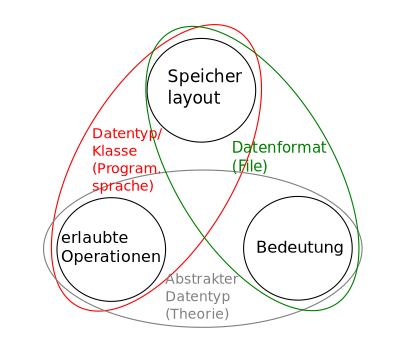
\includegraphics[width=16cm,height=8cm,keepaspectratio]{./Pictures/Datenstrukturdreieck.png}\\
\begin{tabular}{L{4cm} | L{5cm} | L{5.5cm}}
     \multicolumn{1}{c}{\textbf{Abstrakter Datentyp}} & \multicolumn{1}{c|}{} & \textbf{Datentyp in Python} \\ \hline
    Operationen & Bedeutung & Welche Fkt. implementiert man? \\ \hline
    Schlüssel k , Werte v, Array a &  & Hilfsklasse Node \\ \hline
    \verb|a[k] = v| & Speichere v unter dem Schlüssel k oder ersetze Daten, falls k vorhanden & \verb|__setitem__(self, k, v)| \\ \hline
    \verb|v = a[k]| & frage Daten vom Schlüssel k ab, Fehlermeldung falls k nicht vorhanden & \verb|__getitem__(self, k)| \\ \hline
    \verb| a.has_key(k)| & True, wenn k vorhanden & \verb| has_key(self, k| \\ \hline
    \verb|del a[k]| & Lösche Schlüssel k und seine Daten, oder Fehlermeldung, wenn k nicht vorhanden & \verb|__delitem__(self, k)| \\ \hline
    \verb|len(a)| & aktuelle Anzahl der Schlüssel bzw. Schlüssel/Wert-Paare & \verb|__len__(self)| \\ \hline
\end{tabular}\\

k im Prinzip beliebig (Anforderungen später) \\

Fileformate für assoziative Arrays:
\begin{itemize}
    \item lesbar für Menschen und Maschinen (als Textfiles): XML, JSON, YAML
    \item nur lesbar für Maschinen (als Binärfile): HDF5
\end{itemize}

\section{JSON-Format}
\subsection*{7.2.1 Spezifikation des JSON-Formats}
in Backus-Naur-Notation: \\
\begin{tabular}{L{2cm} C{1cm} L{10cm}}
    JSON-file & := & array $|$ \\
    & $|$ & dictionary \\
    array & := & '[' \hspace*{5mm} elements \hspace*{5mm} ']'\\
    & $|$ & '[' \hspace*{1cm} ']'  \hspace*{1cm} \#leeres Array\\
    elements & := & value \\
    & $|$ & value ',' elements \\
    dictionary & := & '\{' \hspace*{5mm} pairs \hspace*{5mm} '\}' \\
    & $|$ & '\{' \hspace*{1cm} '\}'\hspace*{1cm} \#leeres Dictionary \\
    pairs & := & \textcolor{red}{string} ':' value \\
    & $|$ & \textcolor{red}{string} ':' value ',' pairs \\
    string & := & '\grqq' \hspace*{5mm} '\grqq'\hspace*{1.3cm} \#leerer String\\
    & $|$ & '\grqq' characters '\grqq' \\
    value & := & \textcolor{blue}{number} $|$ \textcolor{blue}{string} $|$ \textcolor{blue}{boolean} $|$ \textcolor{blue}{null} $|$ array $|$ dictionary\\
\end{tabular}\\

\textcolor{red}{Schlüssel} \\
\textcolor{blue}{werden als Zeichen im UTF-8 Zeichensatz codiert}

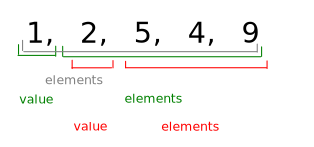
\includegraphics[width=16cm,height=2cm,keepaspectratio]{./Pictures/komischesArray.png}

\subsubsection*{Beispiel für JSON: Studenten-Datenbank}
\begin{minted}{python}
Students = {
    "Fritz Mueller": {
        "Mathematik": [2.0, 1.7, 1.3],
        "ALDA":       1.3
    },
    "Anna Weise": {
        "Mathematik":  [1.0, 1.0, 1.0];
        "Philosophie": 1.3
    }
}
\end{minted}
Einlesen von JSON in Python: json-Modul

\begin{minted}{python}
import json
students = json.load(file("students.json").read().decode("utf_8"))
\end{minted}

\vspace*{1cm}

\begin{tabular}{L{8.5cm} | L{7cm}}
    \textbf{Anforderungen an die Schlüssel :} & Implementation \\ \hline
    \verb|key1 == key2| & sequentielle Suche $\bigO{}(N)$ \\ \hline
    Ordnung \verb|key1 < key2| (impliziert \verb|key1 == key2|) & binäre Suchbäume, binäre Suche $\bigO{}(log N)$ \\ \hline
    \verb|key1 == key2| & Hashtabelle \hspace*{2cm} $\bigO{}(1)$ \\
    \verb|hash(key1) => integer| & \\
\end{tabular}

\vspace*{1cm}



\chapter*{8 Effizientes Sortieren und Suchen}
\addcontentsline{toc}{chapter}{8 Effizientes Sortieren und Suchen}
in $\bigO{}(N)$ (Sortieren) bzw. $\bigO{}(1)$ (Suchen) \\
\begin{itemize}[label={}]
    \item \textbf{Beweis} wenn man nur die Operation \verb|key1 < key2| (Ordnung) zur Verfügung hat, ist Sortieren nicht besser als $\Omega (NlogN)$ möglich
    \item \textbf{Beispiel} Array der Länge 3: kann in $ 6 = 3!$ verschiedenen Sortierungen vorliegen: ABC, ACB, BAC, BCA, CAB, CBA \\
    Ratespiel: mit möglichst wenigen Fragen herausfinden, welche Permutation vorliegt $\Rightarrow$ Suchbaum, Fragebaum \\
    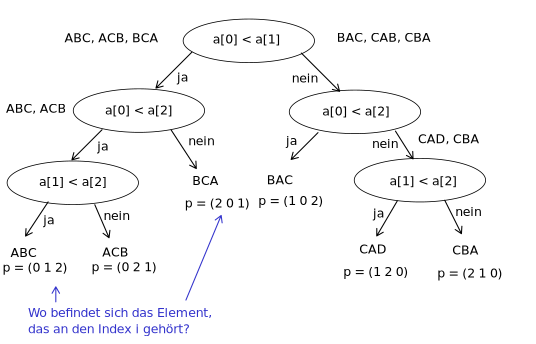
\includegraphics[width=16cm,height=6cm,keepaspectratio]{./Pictures/Fragebaum.png}
\end{itemize}
wenn man p kennt, kann man in $\bigO{}(N)$ sortieren
\begin{minted}{python}
def index_sort(a, p):
    v = [None] * len(a)
    for k in range(len(a)): v[k] = a[p[k]] #O(N)
    return v
\end{minted}
\vspace*{0.5cm}
Wie groß ist der Fragebaum mindestens, wenn wir die Frage so geschickt wie möglich stellen?
\begin{itemize}[label={}]
    \item Um N! Permutationen zu repräsentieren, brauchen wir N! Blätter
    \item Um N! Blätter zu haben, muss der Baum die Tiefe $\Omega (log N!)$ haben
    \item Vereinfachen mit Hilfe der Stirlingschen Formel für große N:
    \[ N! \approx \sqrt{2 \pi N} * \left( \frac{N}{e}\right) ^N\]
    \[ log\hspace*{1mm}N! \approx log\hspace*{1mm} \sqrt{2\pi N} + log\hspace*{1mm} N^N - log\hspace*{1mm} e^N \geq log\hspace*{1mm} \sqrt{2\pi N} + log\hspace*{1mm} N^N\]
    \[ \Omega(log\hspace*{1mm}N!) = \Omega(log\sqrt{2\pi N}) + \Omega(log\hspace*{1mm}N^N) = \boxed{\Omega(N \hspace*{1mm}log\hspace*{1mm}N)}\]
    \item $\Rightarrow$ Sortieren allein mit paarweisen Vergleichen \verb|"key1 < key2"| braucht immer mindestens $\Omega(N \hspace*{1mm} log \hspace*{1mm}N)$ Zeit
    \item $\Rightarrow$ Merge Sort, Quick Sort, Heap Sort sind nicht zu verbessern, ohne zusätzliche Anforderungen in die Schlüssel
\end{itemize}

\section*{8.1 Sortieren in linearer Zeit $\bigO{}$(N)}
\addcontentsline{toc}{section}{8.1 Sortieren in linearer Zeit}
\begin{itemize}
    \item ist einfach, wenn die Schlüssel ganze Zahlen im Bereich $[0, \cdots, M-1]$ \\
    so dass $M \in \bigO{}(N)$ $\Rightarrow$ benutze Array($\infty$) von Arrays $\rightarrow$ ein Array pro Schlüssel (genauer: Queue)
\end{itemize}
\begin{minted}{python}
def integer_sort(a, M):
    bucket = [ [] for k in range(M)] #M leere Queues ([])
    #M = Anzahl der erlaubten Schluessel
    #verteile Raten auf Buckets
    for k in range(len(a)):
        bucket[a[k]._key].append(a[k])  #a[k]._key Element von [0, M-1]

    # sortiertes Array aus den Queues zusammensetzen
    start = 0
    for k in range(M):
        end = start + len(bucket[k])
        [a[start:end] = bucket[k]   #alle Elemente mit Schluessel k in a sortiert einfuegen
        start = end
\end{minted}
Komplexität
\begin{itemize}
    \item line 1-3: $\bigO{}(M)$
    \item line 4-6: $\bigO{}(N)$
    \item line 10-13: $\bigO{}(N) \begin{cases} \text{line 11}: \bigO{}(k) \\ \text{line 12}: \bigO{}(N_k) \\ \text{line 13}: \bigO{}(1) \end{cases}$
\end{itemize}
Schleife über Buckets hat Komplexität: \[\sum_{\Psi = 0}^{M-1} \bigO{}(N_k) = \bigO{}\underbrace{\left(\sum_{k = 0}^{M-1}N_k\right)}_{=N} = \bigO{}(N)\]

$\Rightarrow$ der gesamte Algorithmus ist $\bigO{}(N)$, falls $M \in \bigO{}(N)$ \\

\subsubsection*{Wie kann man das auf beliebige Schlüssel verallgemeinern?}
\begin{itemize}
\item Quantisierung: \verb|quantize(key, M)| $\Rightarrow$ \verb|[0, M-1]| $\widehat{=} q_{\text{key}}$ \\
\hspace*{0.1cm} Ordnungserhaltend: falls \verb|key1| $<$ \verb|key2| $\Rightarrow$ $q_{\text{key1}} \leq q_{\text{key2}}$ \\
wenn eine solche Funktion für keys definiert ist $\Rightarrow$ bucket sort $\in \bigO{}(N)$
\end{itemize}

\section*{8.2 Bucket Sort}
\addcontentsline{toc}{section}{8.2 Bucket Sort}

\begin{minted}{python}
def bucket_sort(a, quantize, d):
    N = len(a)
    M = int(N / float(d)) #Python3 N//d
    # M = Anzahl der Buckets, d = mittlere Zahl von Elementen in jedem Bucket

    bucket = [[] for k in range(M)]
    #Daten auf buckets verteilen
    for k in range(N):
        index = quantize(a[k]._key, M)
        bucket[index].append(a[k])
    #Daten sortiert einfuegen
    start = 0
    for k in range(M):
        insertion_sort(bucket[k])   #sortiere Schluessel mit gleicher Quantisierung
        end = start + len(bucket[k])
        a[start:end] = bucket[k]
        start = end
\end{minted}
Komplexität:
\begin{itemize}
    \item line 2: $\bigO{}(1)$
    \item line 3: $\bigO{}(1)$
    \item line 6: $\bigO{}(M)$
    \item line 8-10 : $\bigO{}(N) \begin{cases}\text{line 8: } \bigO{}(N) & \\ \text{line 9: } \bigO{}(1) & ! \\ \text{line 10: }  \bigO{}(1) & \text{amortisiert}\end{cases}$
    \item line 12: $\bigO{}(1)$
    \item line 13 - 17: $\sum_{k=0}^{M-1} \bigO{}(N_k^2) \begin{cases} \text{line 13: } & \bigO{}(M) \\ \text{line 14: } & \bigO{}(N_k^2) \\  \text{line 15: } & \bigO{}(1)  \\\text{line 16: } & \bigO{}(N_k) \\  \text{line 17: } & \bigO{}(1) \\ \end{cases}$
\end{itemize}
zum Vergleich: integer\_sort:
\[ \sum_{k=0}^{M-1} \bigO{}(N_k) = \bigO{}\left( \sum_{k=0}^{M-1} N_k\right) = \bigO{}(N)\]

jetzt:
\[ \sum_{k=0}^{M-1} \bigO{}(N_k^2) = \sum_{k=0}^{M-1} \bigO{}(1) = \bigO{}(M) \hspace*{0.5cm} \underline{\text{falls }} N_k \in \bigO{}(1) \text{, d.h. unabh. von N und M} \]

\textbf{Wie erreicht man, dass $N_k \in \bigO{}(1)$?}
\begin {enumerate}
    \item Lege $M$ so fest, dass $M \in \bigO{}(N)$: externer Parameter $d \approx 10$ gibt den gewünschten Füllstand jedes Buckets an \\
    \hspace*{3cm} $M = \lfloor \frac{N}{d} \rfloor \in \bigO{}(N)$

    \item Teile Schlüssel so auf die Buckets auf, dass $N_k \approx d$ für alle $k$ \\
    $\Rightarrow$ Komplexität für Bucketsort:
    \[ \sum_{k=0}^{M-1} \bigO{}(N_k^2) = \sum_{k=0}^{M-1} \bigO{}(d^2) = \sum_{k=0}^{M-1} \bigO{}(1) = \bigO{}(M) = \bigO{}(N)\]
    $\Rightarrow$ brauchen quantize(), die das sicherstellt
    \begin{itemize}
        \item einfachster Fall: alle Schlüssel sind reelle Zahlen $\in [0, 1)$, gleichverteilt
        \begin{minted}{python}
def quantize_uniform(key, M):
    return int(key * M)
        \end{minted}
        $\Rightarrow \mathbb{E}_k[N_k] = \frac{N}{M} = \bigO{}(1)$

        \item für andere Wahrscheinlichkeitsverteilungen der Schlüssel muss man die Verteilung kennen, um eine gute quantize-Fkt. zu definieren

        \begin{figure}[htbp]
            \begin{minipage}[t]{10cm}
                \centering
                \begin{enumerate}[label={\alph*)}]
                    \item Formel $p(\text{key}) = \frac{1}{\sqrt{2\pi \sigma^2}} e^{-\frac{1}{2} \frac{\text{key}^2}{\sigma^2}}$  \\
                    \vspace*{5mm}
                    kumulative Verteilungsfunktion:
                    \[ F(\text{key}) = \int\limits_{-\infty}^{\text{key}} p\text{ (key') } d \text{ key } \]
                    \vspace*{5mm}
                    $\Rightarrow$ optimale Quantisierung: int(F(key)*M)

                \end{enumerate}
            \end{minipage}
            \begin{minipage}[t]{6cm}
                \vspace{-1cm}
                \hspace*{-1cm}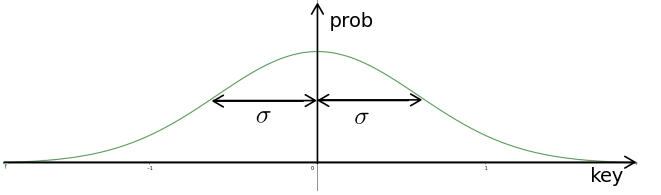
\includegraphics[width=7cm,height=3cm,keepaspectratio]{./Pictures/Graph1.png}\\
                \hspace*{-1cm}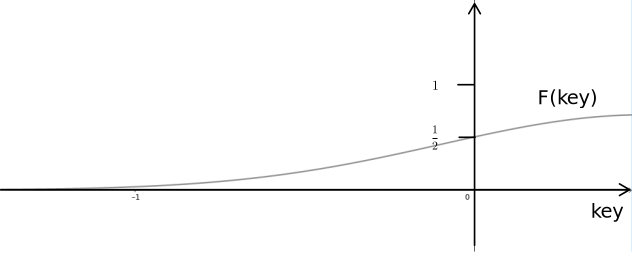
\includegraphics[width=7cm,height=3cm,keepaspectratio]{./Pictures/Graph2.png}\\
            \end{minipage}
        \end{figure}
    \end{itemize}
        \item[b)] keine Formel: empirische Wahrscheinlichkeit $\widehat{=}$ Histogramm \\
        \begin{figure}[htbp]
            \begin{minipage}[t]{10cm}
                \centering
                \vspace{0cm}
                \hspace*{-1cm}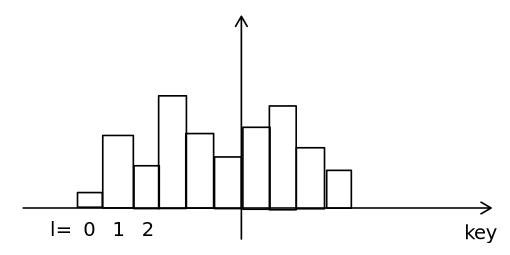
\includegraphics[width=7cm,height=3cm,keepaspectratio]{./Pictures/Balken1.png}\\
            \end{minipage}
            \begin{minipage}[t]{6cm}
            Quantisiere Schlüssel in L Bins\\
            zähle Häufigkeit der Schlüssel für jeden Bin:\\
            \[ h_l \in [0,1]\]
            \end{minipage}
        \end{figure}

        \begin{figure}[htbp]
            \begin{minipage}[t]{10cm}
                \centering
                \vspace{-1cm}
                kumulatives Histogramm $F_e = \sum_{l' = 0}^{l} h_{e'}$ \\
            \end{minipage}
            \begin{minipage}[t]{6cm}
                \hspace*{-1cm}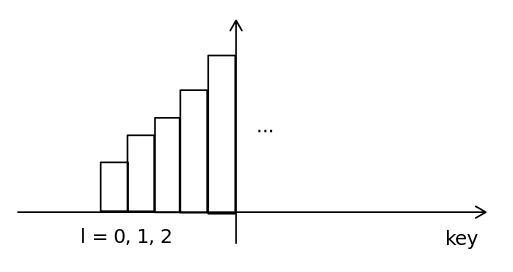
\includegraphics[width=7cm,height=3cm,keepaspectratio]{./Pictures/Balken2.png}\\
            \end{minipage}
        \end{figure}


        $\Rightarrow$ optimale Quantisierung: \hspace*{5mm} l=raw\_quantize(key),
        k = int($F_e * M$)\hspace*{5mm}  F[l] \\

        Hausaufgabe: optimale Quantisierung für Fall a) finden \& bucket\_sort implementieren \\
        Die Quantize-Funktion sollte möglichst billig sein.
\end{enumerate}



\chapter*{9 Hashtabellen}
\addcontentsline{toc}{chapter}{9 Hashtabellen}
Suchen in $\bigO{}(1)$ pro Query (d.h. $\bigO{}(N)$ zum Aufbau der Tabelle) \\

Trick wie bei bucket\_sort: i = hash(key)$\Rightarrow$ ganze Zahl $\in [0,M)$ \\
\hspace*{5mm} Unterschied zu quantize: hash(key) muss $\textbf{nicht}$ die Ordnung erhalten\\
\hspace*{10mm} $\Rightarrow$ mehr Freiheit bei der Auswahl von hash(key)\\
\hspace*{15mm} die selbe Hash-Funktion funktioniert für viele verschiedene Wahrscheinlichkeitsverteilun- \\
\hspace*{15mm} gen der keys.\\

Wertebereich von hash(): U $\widehat{=}$ \glqq Universum\grqq des Schlüssels \\
\hspace*{5mm} z.B. wenn key ein String der Länge 9, 60 erlaubte Zeichen \\
\[ |U| = 60^9 \approx 10^{16}\]
dagegen: $M \in \bigO{}(N) << |U|$ $\Rightarrow$ Viele Schlüssel werden durch hash(key) auf den gleichen Wert\\
\hspace*{15mm} abgebildet $\widehat{=}$ \textbf{Kollision}\\
gute Hashfunktion: Kollision für alle Schlüssel gleich wahrscheinlich \\
\hspace*{15mm} ($\widehat{=}$ bucket\_sort: alle Buckets sind gleich voll) \\

Beispiel: Monatsnummern als Schlüssel \verb|"Januar", "Februar", ..., "Dezember"| \\
hash(key) $\Rightarrow$ key[0] Anfangsbuchstabe: \\

\hspace*{10mm} \textcolor{red}{J} \hspace*{5mm}  F \hspace*{5mm}  \textcolor{blue}{M} \hspace*{5mm}  \textcolor{green}{A} \hspace*{5mm}  \textcolor{blue}{M} \hspace*{5mm}  \textcolor{red}{J} \hspace*{5mm}  \textcolor{red}{J} \hspace*{5mm}  \textcolor{green}{A} \hspace*{5mm}
 S \hspace*{5mm}  O \hspace*{5mm}  N \hspace*{5mm}  D \hspace*{10mm} viele Kollisionen \\

klassisch (Papierformulare) : hash(key)$\Rightarrow$ key[0:3] erste 3 Buchstaben\\
\hspace*{5mm} Jan, Feb, ... \hspace*{2.3cm} keine Kollision, aber M sehr groß ($60^3 = 216000 >> N$) \\

perfekte Hashfunktion: hash(key) $\Rightarrow$ [0,11] \hspace*{5mm} [1,12] \\

\section*{9.1 Bewährte Hashfunktionen}
\addcontentsline{toc}{section}{9.1 Bewährte Hashfunktionen}
Idee: Interpretiere jeden Schlüssel als Bytefolge\\

\textbf{Bernstein:}
\begin{minted}{python}
def b_hash(u):          #u: Array of Bytes
    h = 0
    for i in u:
        h = 33*h + i    # 33 wurde experimentell bestimmt fuer wenig Kollision
    return h
\end{minted}
$h \in [0, \cdots, 2^{32} -1]$ int32 \\
$h \in [0, \cdots, 2^{64} -1]$ int64 \\


\textbf{modifizierte Bernstein:}
\begin{minted}{python}
def mb_hash(u):         #u: Array of Bytes
    h = 0
    for i in u:
        h = 33*h^i      # ^: bitweise XOR
    return h
\end{minted}

\textbf{shift-Add-XOR:}
\begin{minted}{python}
def sax_hash(u):
    h = 0
    for i in u:
        h^= (h << 5) + (h >> 2) + i
    return h
\end{minted}

\textbf{Fowler $|$ Noll $|$ Vo:}
\begin{minted}{python}
def FNV_hash(u):
    h = 2166136261
    for i in u:
        h = (16777619 * h)^i
    return h
\end{minted}
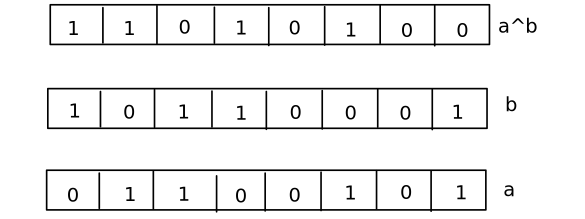
\includegraphics[width=7cm,height=3cm,keepaspectratio]{./Pictures/abArrays.png}

\section*{9.2 Prinzip der Hashtabelle}
\addcontentsline{toc}{section}{9.2 Prinzip der Hashtabelle}
\begin{itemize}
    \item intern: Array der Länge M (dynamisches Array: vergrößere M falls N zu groß wird $\Rightarrow$ später)
    \item speichere Schlüssel key beim Index i =$\underbrace{\text{ hash(key)}}_{0...(2^{32}-1)} \% \underbrace{M}_{>> \bigO{}(N)} \in [0, M-1]$
    \item mache etwas trickreiches bei Kollision
    \begin{itemize}
        \item lineare Verkettung \hspace*{5mm} \glqq offenes Hashing\grqq \glqq geschlossene Adressierung\grqq
        \item offene Adressierung
        \item doppeltes Hashing
    \end{itemize}
\end{itemize}

\section*{9.3 Hashtabelle mit linearer Verkettung}
\addcontentsline{toc}{section}{9.3 Hashtabelle mit linearer Verkettung}
\begin{itemize}
    \item wie bei bucket\_sort: für jeden Index hat man ein Array oder eine verkettete List, wo alle Schlüssel mit demselben Hash landen:
    \begin{minted}{python}
class HashNode:
    def __init__(self, key, value, next):
        self.key = key
        self.value = value
        self.next = next

class HashTabelle:
    def __init__(self):
        self.capacity = ...             # initiales M
        self.size = 0
        self.data = [None] * self_capacity

    def __setitem__(self, key, value):
        i = hash(key) % self.capacity   #bucket finden
        bucket = self.data[i]           #bucket finden
        while bucket is not None:
            if bucket.key == key:       #key war schon vorhanden
                bucket.value = value    # => value ersetzen
                return
            else:
                bucket = bucket.next     #durch verkettete Liste iterieren

        # wenn wir hier landen, war key noch nicht  vorhanden
        # => neues Element einfuegen

        new_node = HashNode(key, value, self.data[i])
        self.data[i] = new_node
        self.size += 1
        ... # hier eventuell die capacity vergroessern

    def __getitem__(self, key):
        i = hash(key) % self.capacity
        bucket = self.data[i]
        while bucket is not None:
            if bucket.key == key:
                return bucket.value
            bucket = bucket.next
        raise keyError(key)
    \end{minted}
\end{itemize}

\subsubsection*{Komplexität der Hash-Tabelle mit linearer Verkettung}
\begin{itemize}
    \item Ausrechnen des Hashs und finden des Buckets: $\bigO{}(1)$
    \item Schlüssel im Bucket suchen: ($N_i$: Länge Bucket i)
    \begin{itemize}
        \item vorhanden $\bigO{}\left(\frac{N_i}{2}\right)$
        \item nicht vorhanden $\bigO{}(N_i)$
    \end{itemize}
    \item mittlere Suchzeit für viele Aufrufe:
    \[ \mathbb{E}[t] = \sum_{i=0}^{M-1} p_i\bigO{}(N_i) \hspace*{3cm} M : \text{capacity} \]
    Annahme: gute Hash-Funktion $\Rightarrow$ Schlüssel gleichmäßig auf die Buckets verteilt\\ $\Rightarrow$ $p_i = \frac{1}{M}, \hspace*{1cm} N_i = \frac{N}{M}$
    \[ \mathbb{E}[t] = \sum_{i=0}^{M-1} \frac{1}{M} \bigO{} \left(\frac{N}{M}\right) = \bigO{} \left(\frac{N}{M^2}\right) \underbrace{\sum_{i=0}^{M-1} 1}_{=M} = \bigO{} \hspace*{-9mm} \underbrace{\left(\frac{N}{M}\right)}_{\text{Füllstand jedes Buckets}}\]
    \item Gesamtzeit soll $\bigO{}(1)$ sein:
    \[ \bigO{}(1)  \stackrel{!}{=} \bigO{}(1) + \underbrace{\bigO{}\left(\frac{N}{M}\right)}_{\bigO{}(1)} \Leftrightarrow M \in \bigO{}(N)\]
$\Rightarrow$ wenn Hashtabelle voll $\Rightarrow$ verdoppele Kapazität M \\
Trick: setze M als Primzahl $\Rightarrow$ keys werden gleichmäßiger verteilt bei hash(key)\%M
\[ M \in \{11, 23, 47, 97, 199, 409, 823, \cdots\}\]
z.B. häufig verwendet für C++ Klasse std::unordered\_map
\end{itemize}

\section*{9.4 Hashtabellen mit offener Adressierung}
\addcontentsline{toc}{section}{9.4 Hashtabellen mit offener Adressierung}
\begin{itemize}
    \item HT mit linearer Verkettung: pessimistisch $\widehat{=}$ es wird viele Kollisionen geben\\ \hspace*{3cm}$\Rightarrow$ jeder Index enthält von vornherein eine Liste von Keys
    \item HT mit offener Adressierung: optimistisch $\widehat{=}$ Kollisionen sind so selten, dass wir keine Liste für jeden Index brauchen\\ \hspace*{3cm}$\widehat{=}$ jeder Index enthält kein oder ein Element
    \item einfachste Variante: \textbf{sequentielles Sondieren}: wenn der gewünschte Index bereits belegt ist $\Rightarrow$ probiere den nächsten bis man einen freien Index findet \\
    Konsequenzen:
    \begin{itemize}
        \item capacity $>$ size notwendig, sonst Endlosschleife
        \item Entfernen von Elementen nicht mit naivem Vorgehen (Element auf None setzen) möglich\\
        \includegraphics[width=10cm,height=4cm,keepaspectratio]{./Pictures/naivesLöschen.png}\\
        statt dessen: gelöschte Elemente als \emph{gelöschte} markieren, damit die Suchkette bei Kollisionen nicht vorzeitig abbricht
    \end{itemize}
    Nachteil: Clusterbildung
    \begin{itemize}
        \item Bereiche, wo alle Indizes belegt sind
        \item Bereiche, wo alle Indizes frei sind\\
        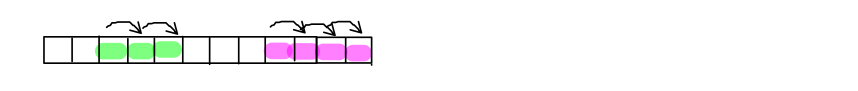
\includegraphics[width=10cm,height=3cm,keepaspectratio]{./Pictures/buntesArray.png}\\
        $\Rightarrow$ Suchzeit linear in der Länge der Cluster, nicht immer $\bigO{}(1)$
    \end{itemize}
    \item verbesserte Variante: doppeltes Hashing: verwende 2. Hashfunktion, um den Ersatzindex\\ \hspace*{5mm}festzulegen $\Rightarrow$ gleichmäßige Verteilung der Belegung
\end{itemize}

Doppeltes Hashing a la Python:
\begin{minted}{python}
def __setitem__(self, key, value):
    i = hash(key)%self.capacity
    h = hash(key)
    while True:
        if self.data[i] is None:    #freies Feld gefunden => key nicht vorhanden
            break
        if self.data[i].key == key: #key gefunden => Daten aktualisieren
            self.data[i].value = value
            return
        #wenn wir hier landen: Kollision(Index i mit anderem key belegt)
        i = (5 * i + 1 + h) % self.capacity
        h //= 32        # h = h // 32

        #wenn wir hier landen wurde der Key nicht gefunden
        h = hash(key)
        i = h % self.capacity
        #zweite Schleife: neues Element einfuegen
        while True:
            if self.data[i] is None or self.data[i].key is None:
                #index ist frei(1. Bedingung) oder als geloescht markiert(2. Bedingung)
                #=> hier gehoert key hin
                self.data[i] = HashNode(key, value)
                self.size += 1
                ... #eventuell muss hier die Kapazitaet optimiert werden
                return
            # index ist schon belegt => neuen Index durch 2. Hashfunktion berechnen
            i = (5 * i + 1 + h) % self.capacity
            h = h // 32
\end{minted}

\begin{minted}{python}
def __getitem__(self, key):
    h = hash(key)
    i = h % self.capacity
    while True:
        if self.data[i] is None:    raise keyError(key)
        if self.data[i].key == key: return self.data[i].value
        i = (5 * i + 1 + h) % self.capacity
        h = h // 32
\end{minted}


\subsubsection*{Komplexität des doppelten Hashings}
\begin{itemize}
    \item mittlerer Füllstand $\alpha = \frac{N}{M} = \frac{\text{size}}{\text{capacity}}$
    \begin{itemize}
        \item erfolglose Suche (Schlüssel nicht vorhanden) \hspace*{5mm}$\Omega(\frac{1}{1-\alpha})$
        \item erfolgreiche Suche (Schlüssel vorhanden) \hspace*{5mm}$\Omega(\frac{1}{\alpha} ln(\frac{1}{1-\alpha}))$
        \begin{figure}[htbp]
            \begin{minipage}[t]{7cm}
                \centering
                \vspace{0cm}
                \begin{tabular}{C{2.5cm}|C{1.3cm}|C{1.3cm}|}
                    $\alpha$ & 0,5 & 0,9 \\ \hline
                    erfolglos & 2 & 10 \\
                    erfolgreich & 1,4 & 2,6
                \end{tabular}
            \end{minipage}
            \begin{minipage}[t]{8cm}
                $\Rightarrow$ verdopple die Kapazität, wenn $\alpha = \frac{2}{3}$ \\
                (in Python: $M \in \{4, 8, 16, 32, ...\}$) \\
                2. Hashfunktion sorgt für gleichmäßige Verteilung
            \end{minipage}
        \end{figure}
    \end{itemize}
\end{itemize}
Anwendung von Hashing zur Suche in Textdateien: Rabin-Karp-Algorithmus
\begin{itemize}
    \item ähnlich zu gleitendem Mittelwert
    \begin{itemize}
        \item naiv: für jede Fensterposition Mittelwert berechnen $\Rightarrow \bigO{}(N*k)$
        \item elegant: bei jeder Fensterposition rechts ein neues Element hinzufügen, links eins entfernen\\
        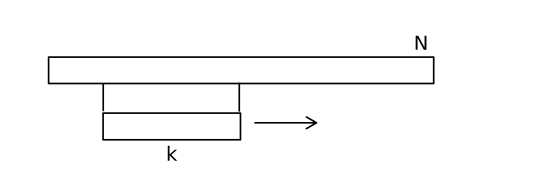
\includegraphics[width=10cm,height=3cm,keepaspectratio]{./Pictures/schiebeArray.png}\\
    \end{itemize}
    \item Suchwort der Länge k $\Rightarrow$ berechne gleitenden Hash für alle Abschnitte der Länge k des Text und vergleiche mit dem Hash des Suchworts
\end{itemize}
\begin{minted}{python}
def rabin_karp_hash(u):
    h = 0
    d,q = 32, 33554393
    for i in u:
        h = (d * h + i) % q
    return h
\end{minted}

\begin{minted}{python}
def rabin_karp_update(c1, c2, k):
    h = (d * h + c2) % q          #rechts ein neues Element hinzufuegen
    h = (h - d ** k * c1) % q   #links eins entfernen
    return h
\end{minted}



\chapter{Rekursion}
\begin{itemize}[label={}]
    \item \hspace*{-1cm} Definition: eine rekursive Funktion ruft sich selbst auf (evtl. indirekt)
    \item \hspace*{-1cm} Eigenschaften:
    \begin{itemize}
        \item jeder rekursive Aufruf hat seinen eigenen Speicher für alle lokalen Variablen
        \begin{minted}{python}
def f(n):
    r = f(n-1) + 1  # Rekursion
    ...
    return r
        \end{minted}
        \item jede rekursive Funktion muss mindestens einen nicht-rekursiven Zweig haben $\widehat{=}$ Basisfall bzw. Rekursionsabschluss (sonst: Endlosrekursion)
        \item jeder rekursive Aufruf muss nach endlich vielen Rekursionsstufen auf den Basisfall zurückgeführt werden \\
        Anzahl der Stufen bis zum Basisfall $\widehat{=}$ Rekursionstiefe
        \item jede Rekursion kann so umprogrammiert werden, dass stattdessen eine/mehrere Schleifen und ein Stack verwendet werden \\
        $\Rightarrow$ Rekursion und Iteration sind gleich mächtig, welche Algorihmen man damit realisieren kann \\
        in der Praxis: Entscheidung, was effizienter und/oder lesbarer ist
    \end{itemize}
\end{itemize}

Arten der Rekursion:
\begin{itemize}
    \item lineare Rekursion: jeder Ausführungspfad (if: else:) enthält höchstens \emph{einen} rekursiven Aufruf $\Rightarrow$ Rekursionskette
    \item Baumrekursion: es gibt Ausführungspfade mit 2 oder mehr rekursiven Aufrufen \\
    $\Rightarrow$ entsteht verzweigter Rekursionsbaum
\end{itemize}

Beispiel: Fibonacci-Zahlen
0, 1, 1, 2, 3, 5, 8, 13, ...\\
\[f_u = f_{u-1} + f_{u-2}; f_0 = 0, f_1 = 1\]

\textbf{Aufgabe: Alg. zur Berechnung der n-ten Fibonacci-Zahl}\\

\textbf{Variante 1:} naive Implementation der Definition:
\begin{minted}{python}
def fib1(n):
    if n <= 1:
        return n
    else:
        return fib1(n-1) + fib1(n-2)
\end{minted}
Nachteil: Baumrekursion\\
\begin{center}
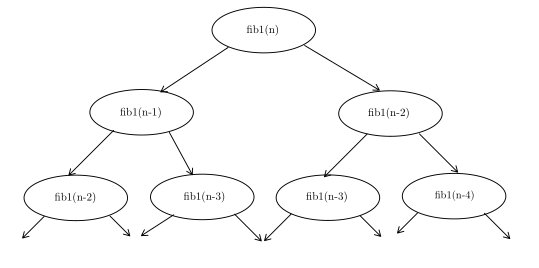
\includegraphics[width=12cm,height=7cm,keepaspectratio]{./Pictures/Fibonacci.png}
\end{center}

Baumtiefe: $\bigO{}(n)$ $\Rightarrow$ Anzahl der Knoten: $\bigO{}(2^n) \widehat{=}$ Komplexität von fib1(n) $\Rightarrow \underline{\text{seeeehr langsam}}$

\textbf{Variante 2:} Umwandlung der Rekursion in Iteration\\

\textbf{Satz:} Jede Rekursion kann mit Hilfe eines Stacks in eine Iteration umgewandelt werden.
\begin{minted}{python}
def fib2(n):
    stack = [n]     #urspruengliches Problem in den Stack legen
    f = 0           #spaeter das Ergebnis
    while len(stack)>0:
        k = stack.pop() #oberstes Teilproblem
        if k <= 1:      #Rekursionsabschluss => Berechnung
            f += k
        else:           #Rekursion => neue Teilprobleme in den Stack
            stack.append(k-1)
            stack.append(k-2)
    return f
\end{minted}

Anzahl der Iterationen = Anzahl rekursive Aufrufe in fib1(n)\\
$\Rightarrow$ Komplexität immer noch $\bigO{}(2^n) \Rightarrow$ Umwandlung in Iteration allein verbessert nie die Komplexität\\

\textbf{Variante 3:} effizienter durch Vermeidung wiederholter Berechnungen der selben Fibonacci-Zahl: \emph{course-of-values-Rekursion} \\

Aufruf für k läuft rekursiv nur von den Aufrufen für k-1, k-2, ..., k-c ab, für konstante c $\Rightarrow$ trifft hier zu mit c = 2

$\Rightarrow$ man kann die Baumrekursion vermeiden, indem man die Zwischenergebnisse so lange speichert, bis sie nicht mehr benötigt werden. \\

Hier: speichere $f_k$, bis $f_{k+2}$ berechnet ist
\begin{minted}{python}
def fib3(n):
    f_n_plus_1, f_n = fib3_impl(n)
    return f_n

def fib3_impl(n):
    if n == 0:
        return 1, 0
    else:
        f_n, f_m_minus_1 = fib3_impl(n-1)
        return f_n + f_n_minus_1, f_n
\end{minted}
entscheidend: Hilfsfunktion ist linear rekursiv $\widehat{=}$ nur 1 rekursiver Aufruf \\
$\Rightarrow$ statt Rekusionsbaum in fib1(n) $\Rightarrow$ Rekusionskette\\
$\Rightarrow$ Komplexität $\bigO{}(N)$, effizienter\\

\textbf{Variante 4:} Umwandeln in Endrekursion $\widehat{=}$ lineare Regression, wo der rekursive Aufruf der letzte Befehl vor dem \emph{return} ist \\

\textbf{Satz:} Jede \emph{Course-of-values-Rekursion} kann in Endrekursion umgeschrieben werden.

\begin{minted}{python}
def fib4(n):
    return fib4_impl(1, 0, n)   #f1, f0, gesuchte Fibonacci-Zahl

def fib4_impl(f_k, f_k_minus_1, counter):
    if counter == 0:            #Rek-Abschluss
        return f_k_minus_1
    else:
        return fib4_impl(f_k + f_k_minus_1, f_k, counter - 1)   #Endrekursion
\end{minted}

\textbf{Variante 5: }Iterative Version ohne Stack\\

\textbf{Satz:} Jede endrekursive Funktion kann ohne Stack in Iteration umgewandelt werden. \\
Idee:
\begin{itemize}
    \item Jeder rekursiveAufruf hat sein eigenes, privates Set lokaler Variablen
    \item ist der rekursive Aufruf der letzte Befehl, werden lokale Variablen \emph{danach} nicht mehr benötigt
\end{itemize}
$\Rightarrow$ wir können die lokalen Variablen für den rekursiven Aufruf recyclen $\widehat{=}$ Überschreiben von Variablen in jeder Schleifeniteration \\

$\rightarrow$ Manche Programmiersprachen (LISP, SCHEME) machen diese Optimierung automatisch\\

\begin{minted}{python}
def fib5(n):
    f_k, f_k_minus_1 = 1, 0
    while n > 0:
        f_k, f_k_minus_1 = f_k + f_k_minus_1, f_k
        n -= 1
    return f_k_minus_1
\end{minted}
n Iterationen $\Rightarrow$ $\bigO{}(n)$\\

\textbf{Variante 6:} (Hausaufgabe) Komplexität $\bigO{}(log N)$ \\

\section{Umwandlung von Rekursion in Iteration}
\textbf{Beispiel für Umwandlung von Rekursion in Iteration mit Stacks}
\begin{minted}{python}
def tree_sort(node, a):     #Aufgabe: geg.Suchbaum, Schluessel in aufsteigender Reihenfolge auslesen und in Array a kopieren
    if node is None: return     #Rekursionsabschluss
    tree_sort(node.left, a)     # kleine Schluessel
    a.append(node.key)          # "mittleren Schluessel" einfuegen
    tree_sort(node.right, a)    #grosse Schluessel
\end{minted}
in-order-trav...

\begin{minted}{python}
def tree_sort_iterative(node, a):
    stack = []
    traverse_left(node, stack)
    while len(stack) > 0:
        current = stack.pop()
        a.append(current.key)
        traverse_left(current.right, stack)
\end{minted}
\begin{minted}{python}
def traverse_left(node, stack):
    while node is not None:
        stack.append(node)
        node = node.left
\end{minted}

Komplexität: $\bigO{}(2^P) = \bigO{}(2^{log N}) = \bigO{}(N)$ falls Baum balanciert \\

\section{Komplexitätsberechnung rekursiver Algorithmen}
\[ T(n) = \underbrace{a_1 * T\left(\frac{N}{b_1}\right)}_{\text{Aufwand für $a_1$ rekursive Teilprobleme der Größe N/$b_1$}} + \cdots + \underbrace{a_n* T\left(\frac{N}{b_n}\right)}_{a_n \text{Teilprobleme der Größe} \frac{N}{b_n}} + \underbrace{f(N)}_{\text{Aufwand der aktuellen Fkt}}\]

fib1(n) : 1 Aufruf(n-1), 1 Aufruf(n-2) $\Rightarrow$ 2 Aufrufe $\bigO{}(N)$ \\
\hspace*{5cm} $n_1 = 2, b_1 = 1, k = 1$ \\
Ausrechnen durch
\begin{itemize}
    \item Substitutionsmethode (\glqq händisch\grqq) $\Rightarrow$ später
\end{itemize}
    \subsection{Mastertheorem}
    \begin{itemize}
    \item \textbf{Mastertheorem} (einsetzen): $T(n) = a* T\left(\frac{N}{b}\right) + f(n)$
    \begin{itemize}[label={}]
        \item Definiere Rekursionsexponent: $\rho = log_b(a)$
        \item \textbf{Fall 1}: $f(N)$ sehr effizient: $f(N) \in \bigO{}(N^{\rho-\epsilon}), \epsilon > 0$ \\
        $\Rightarrow$ $T(N) \in \Theta(N^\rho)$Rekursion dominiert
        \item \textbf{Fall 2}: $f(N)$ so effizient wie Rekursion: $f(N) \in \Theta(N^\rho)$ \\
        $\Rightarrow T(N) \in \Theta(N^\rho * logN) \Rightarrow$ Rekursion und f(N) tragen bei
        \item \textbf{Fall 3}: $f(N)$ nicht so effizient: $f(N) \in \Omega(N^{\rho + \epsilon}), \epsilon > 0$ \\
        \hspace*{5cm} $a f\left(\frac{N}{b}\right) \leq c* f(N)$ mit $c < 1$ \\
        $\Rightarrow T(N) \in \Theta(f(N)) \Rightarrow f(N)$ dominiert
    \end{itemize}
    \item \textbf{Beispiel} Merge Sort: $T(N)\ =\ \underbrace{2 T \ \left(\frac{N}{2}\right)}\hspace*{0.7cm} +\hspace*{0.7cm} \underbrace{\Theta\ (N)}$\\
    \begin{tabular}{L{4cm} L{3cm} L{3cm}}
        $a=2, b=2$ & rekursive Aufrufe für linke und rechte Hälfte & Zusammenfügen der sortierten Hälften\\
    \end{tabular}\\
    \hspace*{1cm} $\rho = log_b(a) \ = \ log_2(2) \ = \ 1 \ \Rightarrow \ f(N)\ \in \ \Theta(N^2) \ = \ \Theta(N)$\\
    $\Rightarrow$ Fall 2  \hspace*{1cm} $T(N)\  \in\  \Theta(N^{\rho}\ log\ N)\ =\ \boxed{\Theta(N\ log(N))}$ wie bekannt
\end{itemize}

    \subsection{Substitutionsmethode}
    \subsubsection*{Händisches Berechnen mittels Substitutionsmethode}
    \begin{itemize}
        \item \textbf{Beispiel}: Merge Sort, wo wir in zwei ungleich große Teilprobleme aufspalten \\
        \[ T(N)\ =\ T\left(\frac{N}{3}\right)\ +\ T\left(\frac{2N}{3}\right)\ +\ \Theta(N)\]
        zeige jetzt: ungleiche Aufteilung ändert nicht die Komplexität
        \item \textbf{Rekursionsbaum}:\\
        \begin{center}
        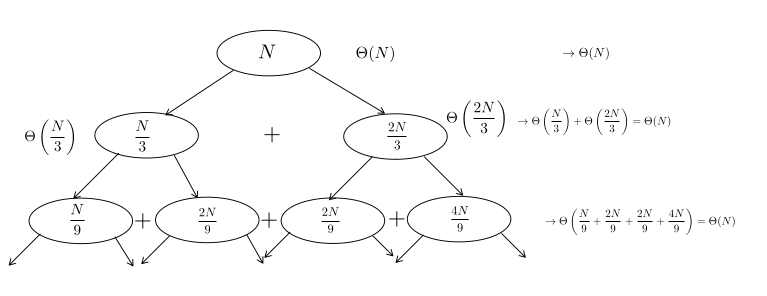
\includegraphics[width=15cm,height=8cm,keepaspectratio]{./Pictures/Substitutionsmethode.png}
        \end{center}
        Berechnen des Aufwands der eigentlichen Berechnung in jedem Knoten ohne Rekursion\\
        $\Rightarrow$ pro Ebene: $\Theta(N) \ \Rightarrow$ Gesamtaufwand $\Theta(N*D)$ $D\ \dots$ Tiefe des Baums \\
        Rekursion endet, wenn Knoten nur 1 Element enthält: $\left(\frac{2}{3}\right)^D * N = 1$\\
        \hspace*{1cm} $\Rightarrow\ D\ =\ log_{3/2}(N)\ = \ \bigO{}(log\ N)$
        \item Vermutung: $T(N)\ \in\ \bigO{}(log_{3/2}(N)\ *\ c*N)\ =\ \bigO{}\ (log\ N\ *\ N)$\\
        falls die Vermutung gilt, gilt für großes N:
        \[ T(N)\ \leq\ d\ *\ N\ *\ \underbrace{log_2(N)}_{ld}\ \text{Definition der O-Notation mit passender Konstante d}\]
        Einsetzen in Rekursionsformel
        \[ T(N)\ =\ T\left(\frac{N}{3}\right)\ +\ T\left(\frac{2N}{3}\right)\ +\ c*N \ \leq d \frac{N}{3} ld\left(\frac{N}{3}\right)\ + d\frac{2N}{3} ld\left(\frac{2N}{3}\right)\ +\ c*N\]
        \[ \leq d*\frac{N}{3} ld(N)\ -\ d\frac{N}{3} ld(3)\ +\d*\frac{2N}{3} ld(N)\ -\ d\frac{2N}{3} \underbrace{ld(2)}_{=1}\ - d\frac{2N}{3} ld(3)\ +\ c*N \]
        \[ d\ N\ ld(N)\ \underbrace{-\ d\ N\ \left(ld(3)\ -\ \frac{2}{3}\ \right)\ +\ c*N}_{\text{sollte} \leq 0\text{sein}} - d\ \not N\  \left(ld(3)\ - \ \frac{2}{3}\ \right)\ +\ c*\ \not N\ \leq\ 0\]
        mit:
        \hspace*{1cm} $d\ \left(\ ld(3)\ -\ \frac{2}{3}\right)\ +\ c* \not N \leq 0$ und $d\ \left(\ ld(3)\ -\ \frac{2}{3}\right)\ \geq c$ immer erreichbar, weil beliebig groß gewählt werden darf
        \[ \leq d\ N\ ld(N) \Rightarrow \text{Vermutung bestätigt}\]
        $\Rightarrow T(N)\ \in\ \bigO{}(N\ log\ N)\  \text{w. z. b. w.}$
    \end{itemize}

%TODO fehlt...



\chapter{Graphen und Graphenalgorithmen}
\section{Einführung}

\begin{itemize}
    \item Entstehung des Graphenformalismus: Königsberger Brückenproblem

    \begin{figure}[htbp]
        \begin{minipage}[t]{8cm}
            \centering
            \vspace{0cm}
            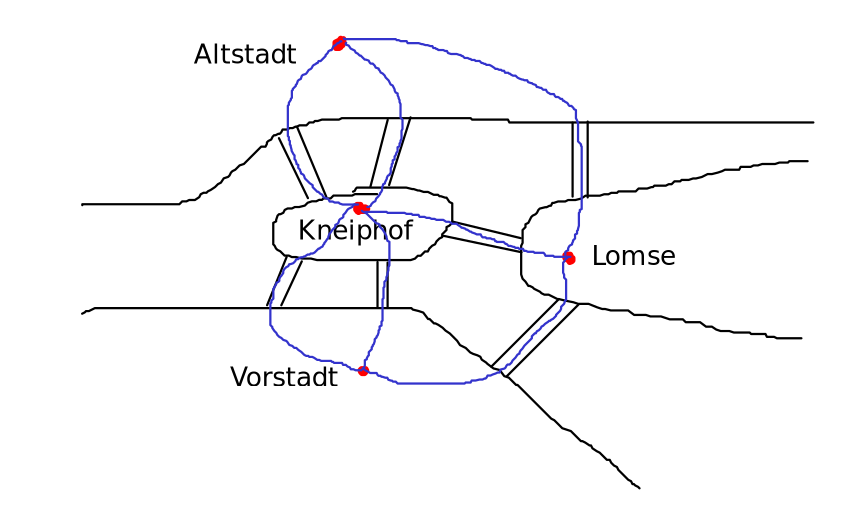
\includegraphics[width=8cm,height=7cm,keepaspectratio]{./Pictures/Koenigsberg.png}\\
            $G = (V, E)$\\
            $E \subset V \times V$
        \end{minipage}
        \begin{minipage}[t]{8cm}
            \vspace{0cm}
            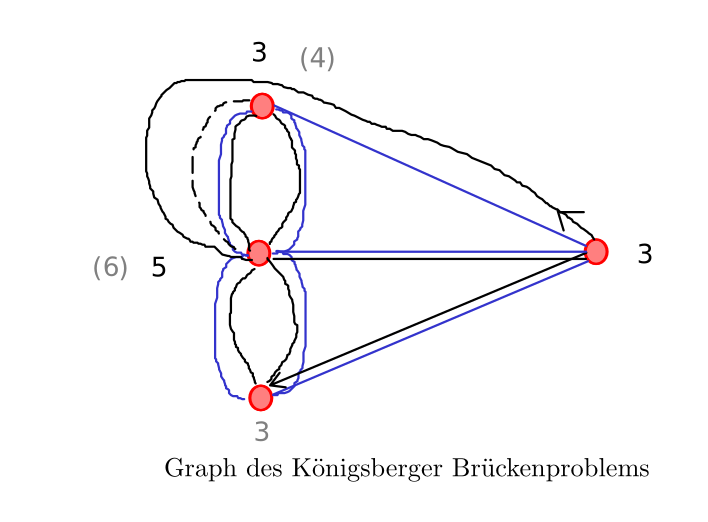
\includegraphics[width=8cm,height=5cm,keepaspectratio]{./Pictures/Brueckengraph.png}\\
            V $\dots$ Vertices, Knoten, E $\dots$ Edges, Kanten\\
            Multigraph $\widehat{=}$ zwei Knoten können durch mehrere Kanten verbunden sein
        \end{minipage}
    \end{figure}

    \item Antwort auf Königsberger Brückenproblem: \glqq Kann man mit einem Spaziergang alle Brücken genau einmal überqueren?\grqq $\Rightarrow$ Nein
    \begin{itemize}
        \item Anforderung: jeder Knoten (Stadtteil), der betreten wird, muss auch wieder verlassen werden $\Rightarrow$ zwei Kanten nötig, oder allg.: eine gerade Anzahl an Kanten
        \item Ausnahmen: Start- und Endpunt des Spaziergangs, falls verschieden
    \end{itemize}
\end{itemize}

\section{Definitionen}
\begin{itemize}
    \item \textbf{Arten von Graphen}: ungerichtete und gerichtete
    \begin{itemize}
        \item ungerichtet: $u, v \in V \hspace*{1cm} (u,v) \in E \Rightarrow (v, u) \in E$ Kanten ohne Richtung
        \item gerichtet: $u, v \in V \hspace*{1cm} (u,v) \in E \Rightarrow$ $(v, u)$ nicht notwendigerweise vorhanden, zeichne Kanten als \textbf{Pfeile}
        \end{itemize}
        \item \textbf{Grad eines Knotens}:
        \begin{itemize}
        \item ungerichtet: Anzahl der Kanten, die in einem Knoten anliegen, \glqq degree\grqq \\
        $deg(u) = | \{ \ v\  | \ (u,v)\  \in \ E\ \}| \Leftrightarrow (v,u) \in E$
        \item gerichtet:
        \begin{itemize}
            \item in-degree: Anzahl der Kanten, die im Knoten enden
            \item out-degree: Anzahl der Kanten, die im Knoten beginnen
            \item $in\_deg(u) = |\{ \  v \ |\  (v,u) \ \in E\ \}|, \ out\_deg(u) = |\{\  u\  |\  (u,v) \ \in E\ \}|$
        \end{itemize}
        \end{itemize}
            \item vollständiger Graph: alle möglichen Kanten existieren auch, jeder Knoten ist mit jedem Knoten \emph{direkt} verbunden\\
            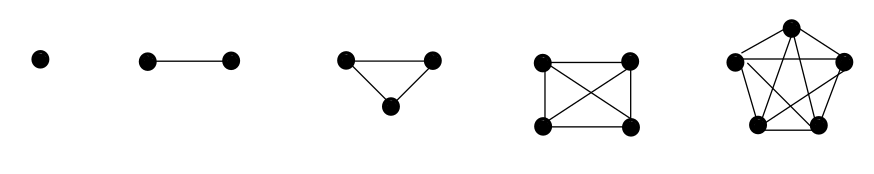
\includegraphics[width=15cm,height=6cm,keepaspectratio]{./Pictures/vollstGraphen.png}\\
            ungerichteter vollständiger Graph: $|E| = \frac{|V|\  ( |V|\  -\ 1)}{2}$\\
            Rätsel: jeder stößt auf Party mit jedem an, es macht 78 mal \glqq pling\grqq \\
            Wie viele Gäste waren da? \hspace*{2cm} $|V| = 13$
            \item Subgraphen: $G' = (V', E')$ ist Subgraph von $G = (V, E)$, wenn :\\ $V'\subseteq V\ ,\  E' \subseteq E$ und für alle $(u, v) \in E'$ muss $(u, v) \in V'$ \\

            Spezialfälle:
            \begin{itemize}
            \item $V' = V$: aufspannender Teilgraph
            \item lösche zuerst Knoten $V' \subset V$, lösche dann alle Kanten \\
            $(u, v)$ wo $u$ oder $v$ $\not \in V'$ $\Rightarrow$ \emph{induzierter Teilgraph}
            \end{itemize}
            \item Wege in Graphen: rekursive Definition
            \begin{itemize}
            \item ein einzelner Knoten $v \in V$ ist ein trivialer Weg der Länge 0
            \item ist eine Folge $(v_1, \cdots, v_{k-1})$ ein Weg und die Kante $(v_{k-1}, v_k)\in E$ existiert, so ist\\ $\underbrace{(v_1, \cdots v_{k-1}, v_k)}_{\text{Länge (k-1)} \widehat{=} \text{Zähle die Kanten im Weg}}$ \hspace*{-1cm}auch ein Weg
            \end{itemize}
            \item Pfad: Weg, wo jeder Knoten \emph{höchstens ein mal} vorkommt ($\widehat{=}$ keine Kreuzungen)
            \item Zyklus: Weg, wo $v_1 = v_k$ Anfangs- gleich Endknoten
            \item Kreis: Zyklus ohne Kreuzung $(v_1, \dots, v_{k-1}, v_k)$ ist Zyklus \\
            d.h. $v_1 = v_k$ und $(v_1, \dots, v_{k-1})$ ist Pfad
            \item Erreichbarkeit $u \rightsquigarrow v$ \hspace{5mm} \glqq v ist erreichbar von u\grqq $\Leftrightarrow$ es gibt einen Weg $(u, \dots, v)$ \\
            $\begin{rcases}
                \text{ungerichtet:} & u \rightsquigarrow v\  \Rightarrow\  v \rightsquigarrow u\\
                \text{gerichtet:} & \text{gilt das nicht unbedingt}
            \end{rcases}$ Konsequenzen für Zusammenhangskomponenten (später)

        \newpage
        \end{itemize}
        \begin{figure}[htbp]
            \begin{minipage}[t]{12cm}
                \vspace{0cm}
                \begin{itemize}
                    \item \textbf{Eulerweg}: enthält jede Kante genau ein Mal \\
                    (Brückenproblem: \glqq Kante\grqq $\widehat{=}$ \glqq Brücke\grqq ) \\
                    Beispiel: Haus vom Nikolaus
                    \item \textbf{Hamiltonweg}: Weg, der alle \emph{Knoten} genau einmal enthält \\
                    Bsp.: Haus vom Nikolaus:
                    \item \textbf{Hamiltonkreis}: Kreis, der alle Knoten genau einmal enthält (außer Anfang/Ende)\\
                    \hspace*{5mm}Bsp.: Haus vom Nikolaus \\
                    Beispiel: Problem des Handlungsreisenden: Suche den kürzesten Hamiltonkreis, der gegebene Städte verbindet $\Rightarrow$ Prototypisches Problem für \emph{NP-vollständig}
                \end{itemize}
            \end{minipage}
            \begin{minipage}[t]{4cm}
                \vspace{-0.5cm}
                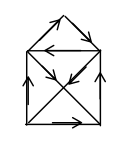
\includegraphics[width=2cm,height=2cm,keepaspectratio]{./Pictures/HausmitPf.png}\\
                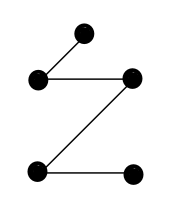
\includegraphics[width=2cm,height=2cm,keepaspectratio]{./Pictures/Hamiltonweg.png}\\
                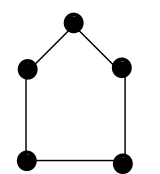
\includegraphics[width=2cm,height=2cm,keepaspectratio]{./Pictures/Hamiltonkreis.png}\\
            \end{minipage}
        \end{figure}

        \section{Planare Graphen, ebene Graphen}
        \begin{itemize}
        \item planar: Graph kann ohne Überkreuzungen in der Ebene gezeichnet werden
        \item eben: wenn tatsächlich so gezeichnet\\
        \includegraphics[width=14cm,height=5cm,keepaspectratio]{./Pictures/plan_ebe_Gr.png}\\
        \begin{figure}[htbp]
            \begin{minipage}[t]{12cm}
                \vspace{0cm}
                \begin{itemize}
                    \item ebener Graph definiert eindeutig Flächen / Regionen in der Ebene
                    \item dualer Graph: jede Region ist ein dualer Knoten\\
                    duale Knoten werden durch Kanten verbunden, wenn die Regionen eine gemeinsame Grenze haben (\emph{nicht nur} gemeinsamen Knoten)
                \end{itemize}
            \end{minipage}
            \begin{minipage}[t]{4cm}
                \vspace{-0.5cm}
                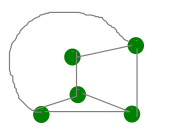
\includegraphics[width=2cm,height=2cm,keepaspectratio]{./Pictures/gruenerGraph.png}\\
            \end{minipage}
        \end{figure}

        Eulersche Gleichung: $|V| - |E| + |F| = 2$
    \end{itemize}
    \begin{itemize}
    \item \textbf{Baum}: \emph{zusammenhängender Graph}, der keine Zyklen enthält \\
    $\forall u,v : u \rightsquigarrow v\  \Rightarrow$ bei $|V|$ Knoten, $|E| = |V| - 1$ Kanten\\
    \begin{flushright}
    \vspace*{-2cm}
    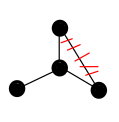
\includegraphics[width=1.5cm,height=1.5cm,keepaspectratio]{./Pictures/Baum_def.png}
    \end{flushright}
    \item \textbf{Spannbaum}: Baum als Subgraph eines Graphen G, der alle Knoten enthält (zusammenhängend $\Leftrightarrow$ G auch zusammenhängend) \\
    \begin{itemize}
        \item Problem: minimaler Spannbaum $\widehat{=}$ kürzeste Kanten $\Rightarrow$ später \\
        \item   wenn G nicht \emph{zusammenhängend}: Wald (hat keine Zyklen) $\widehat{=}$ Menge von Spannbäumen (einer pro Zusammenhangskomponente)
    \end{itemize}
    \end{itemize}

    \section[Graphendatenstrukturen, Adjazenzlisten, Adjazenzmatrizen]{Repräsentation von Graphen}

    \subsection*{Adjazenzmatrix}
     $ A\  (\ |v|\ \times \ |v|\ )\ :\  a_{i,j} = \begin{cases} 1 & \text{wenn} (u_i, u_j) \in E \\
    0  & \text{sonst}\end{cases}$
    \begin{itemize}
        \item ungerichteter Graph: A immer symmetrische Matrix: $A = A^T$ \\
        \hspace*{1cm} $a_{ij} = a_{ji}$ \hspace*{2mm} weil \hspace*{2mm} $(u_i, u_j) \in E \Rightarrow (u_j, u_i) \in E$
        \item gerichteter Graph: A im allgemeinen nicht symmetrisch
        \item Vorteil:
        \begin{itemize}
            \item man kann in Graphalgorithmen Matrix-Funktionen benutzen
            \item Speicher-effizient für dicht besetzte Graphen $| E | \ \in \bigO{}(|V|^2)$
        \end{itemize}
        \item Nachteil:
        \begin{itemize}
            \item Speicherverschwendung für dünn besetzte Graphen \\
            viele $a_{i,j} = 0$ \hspace*{1cm} $|E| \in \bigO{}(|V|)$ \hspace*{1cm} (z.B. planare Graphen)
        \end{itemize}
    \end{itemize}

    \begin{figure}[htbp]
        \begin{minipage}[t]{4cm}
            \vspace{0cm}
            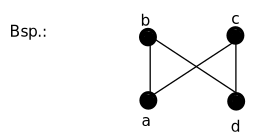
\includegraphics[width=4cm,height=3cm,keepaspectratio]{./Pictures/Adjazenzmatrix.png}
        \end{minipage}
        \begin{minipage}[t]{12cm}
            \vspace{0.0cm}
            $A = \underbrace{\begin{pmatrix}
            0 & 1 & 0 & 1 \\
            1 & 0 & 1 & 0 \\
            0 & 1 & 0 & 1 \\
            1 & 0 & 1 & 0 \\
            \end{pmatrix} }_{a, b, c, d}$ \hspace*{1cm} $al = [[b, d], [a, c], [b, d], [a,c]]$
        \end{minipage}
    \end{figure}

    \subsection*{Adjazenzlisten}
    Array von Arrays: ein Array pro Knoten enthält die Indizes der Nachbarn
    \begin{itemize}
        \item Vorteil:
        \begin{itemize}
            \item speichereffizient für dünn besetzte Graphen ($a_{ij} = 0$ nicht explizit gespeichert), \glqq dünn besetzte Matrixdarstellung\grqq
            \item elegante Schleife über alle Nachbarn und alle Kanten
            \begin{minted}{python}
for node in graph:      #graph = Adjazenzliste
    for neighbor in node:
        #verarbeiten Kante (node, neighbor)
            \end{minted}
        \end{itemize}
        \item Nachteil:
        \begin{itemize}
            \item manche Operationen umständlicher
            \item man muss bei ungerichteten Graphen auf die Symmetrie achten
        \end{itemize}
    \end{itemize}

    \subsection*{Transponierter Graph}
    \begin{itemize}
        \item für alle Kanten: Richtung invertiert \hspace*{1cm} $G^T$
        \item bei ungerichteten Graphen: wieder der gleiche Graph
        \item Adjazenzmatrix: $A_{GT} = A_G^T$
        \item Adjazenzliste:
        \begin{minted}{python}
def transpose_graph(graph):
    gt = [[] for u in graph ]
    for node in range(len(graph)):
        for neighbor in graph[node]:
            gt[neighbor].append(node)
    return gt
        \end{minted}
    \end{itemize}

    \section{Iterieren durch Graphen}
    \subsection*{Traversieren von Graphen}
    \begin{itemize}
        \item alle Knoten in einer sinnvollen Reihenfolge (genau einmal) besuchen
        \item Arten:
        \begin{itemize}
            \item Tiefensuche (depth first search, DFS) $\Rightarrow$ erst in die Tiefe, dann zu den anderen Nachbarn
            \item Breitensuche (breadth first search, BFS) $\Rightarrow$ erst zu allen Nachbarn, dann in die Tiefe
        \end{itemize}
    \end{itemize}

    \subsection*{Tiefensuche – DFS}
    \addcontentsline{toc}{subsection}{Tiefensuche, Breitensuche}
    \begin{minted}{python}
def dfs(graph, startnode):           # graph: zusammenhaengenge Adjazenzliste
    visited = [False] * len(graph)   # Flags, welche Knoten schon besucht
    def visit(node):
        if not visited[node]:
            visited[node] = True
            print(node)                  # in der Praxis: anwendungsrelevante Rechnung
            for neighbor in graph[node]: # Adjazenzliste regelt Reihenfolge
                visit(neighbor)
            # print(node)
    visit(startnode)
    \end{minted}

    \newpage
    \begin{figure}[htbp]
        \begin{minipage}[t]{11cm}
            \vspace{0cm}
            \begin{minted}{python}
dfs(graph, 0)
0   #5
1   #6
3   #2
2   #3
5   #4
6   #1
4   #0
=> disovery order / pre-order: verarbeite jeden Knoten VOR seinen Nachbarn -> Hinweg der Rekursion
# => finishing order / post-order: auf dem Rueckweg der Rekursion nach den Nachbarn
            \end{minted}
        \end{minipage}
        \begin{minipage}[t]{6cm}
            \vspace{0.0cm}
            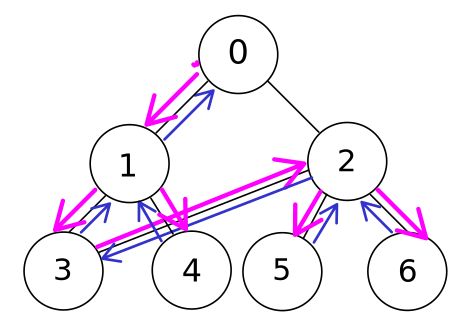
\includegraphics[width=6cm,height=4cm,keepaspectratio]{./Pictures/DFS.png}
        \end{minipage}
    \end{figure}

    \subsubsection*{Anwendungen}
    \begin{figure}[htbp]
        \begin{minipage}[t]{8cm}
            \vspace{0cm}
        \textbf{pre-order traversal}
        \begin{itemize}
            \item Graphen kopieren: kopiere erst den Knoten, dann seine Nachbarn und Kanten
            \item Zusammenhangskomponenten in Graphen finden \\
            (Variante von DFS $\Rightarrow$ später)
            \item wenn Graph schon Baum ist: Abstand jedes Knotens von Wurzel
            \item Taschenrechner (Graph ist Parse tree):\\
            Drucken des Ausdrucks in Funktionsschreibweise  add(3, mul(4,2))
            [Operationsschreibweise: in-order Traversal 3 + (4 * 2)]
        \end{itemize}
        \end{minipage}
        \begin{minipage}[t]{8cm}
        \vspace{0.0cm}
        \textbf{post-order traversal}
        \begin{itemize}
            \item Graphen löschen: erst Nachbarn löschen, dann den Knoten
            \item Bestimme topologische Sortierung eines gerichteten Graphen ($\Rightarrow$ später)
            \item wenn Graph schon Baum ist: Abstand jedes Knotens von den Blättern
            \item Taschenrechner (Graph ist Parse tree):\\
            Auswertung / Berechnung des Ausdrucks
        \end{itemize}
        \end{minipage}
    \end{figure}

    \begin{itemize}
        \item Beides: Weg aus einem Labyrinth $\Rightarrow$ Hausaufgabe\\
        pre-order: Vorwärtsweg \hspace*{1.5cm} $\Leftrightarrow$\hspace*{1.5cm} post-order: Backtracking aus Sackgassen
    \end{itemize}

    Für viele Anwendungen brauchen wir zusätzliche Informationen über den Graphen, die DFS sammeln kann: z.Zt. Flags \emph{visited} \\
    sinnvoll z.B.
    \begin{itemize}
        \item Reihenfolge der Pre- oder Postorder
        \item Elternknoten bei der DFS / von wo wurde node erreicht
    \end{itemize}
    $\Rightarrow$ property maps: Arrays, die für Knoten i und prop[i] die Info speichern

    \subsubsection*{Tiefensuche mit property maps}
    \begin{minted}{python}
def dfs(graph, startnode):
    visited = [False] * len(graph)
    parents = [None] * len(graph)   #zusaetzliche property maps
    disovery_order = []             #
    finishing_order = []            #

    def visit(node, parent):
        if not visited[node]:
            visited[node] = True
            parents[node] = parent
            discovery_order_append(node)
            for neighbor in graph[node]:
                visit(neighbor, node)
            finishing_order.append(node)
    visit(startnode, None)
    return parents, discovery_order, finishing_order
    # Benutze in anderen Algorithmen
    \end{minted}

    Am Beispiel des letzten Graphen:
    parents = [None, 0, 3, 1, 1, 2, 2]\\
    \hspace*{8.3cm} 0, 1, 2, 3, 4, 5, 6\\

    Konvention: Parent des Startnode ist der Startnode selbst $\Rightarrow$ visited Array kann eingespart werden\\


    \subsection*{Breitensuche}
    \begin{minted}{python}
    from collections import deque
    def bfs(graph, startnode):
        parents = [None] * len(graph)
        parents[startnode] = startnode
        q = deque()
        q.append(startnode)

        while len(q) > 0:
            node = q.popleft()                              #q.popright() => Tiefensuche
            print(node)
            for neighbor in graph[node]:
                if parents[neighbor] is None:   #neighbor node nicht besucht
                    parents[neighbor] = node
                    q.append(neighbor)
    \end{minted}

    \begin{figure}[htbp]
        \begin{minipage}[t]{11cm}
        \vspace{0cm}
            \begin{minted}{python}
bfs(graph, 0)
0
1
2
3
4
5
6
=> level order nach Abstand vom startnode und von links nach rechts
            \end{minted}
        \end{minipage}
        \begin{minipage}[t]{6cm}
        \vspace{0.0cm}
        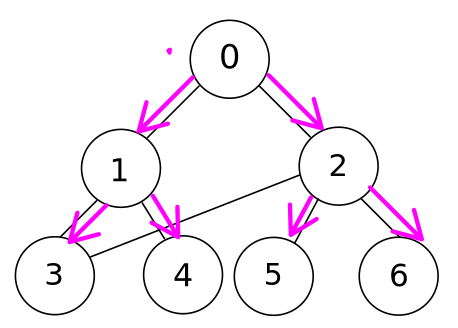
\includegraphics[width=6cm,height=4cm,keepaspectratio]{./Pictures/BFS.png}
        \end{minipage}
    \end{figure}

\newpage
    \subsection*{Anwendungen von Tiefensuche – Damenproblem (beim Schach)}
    \textbf{Aufgabe}: Platziere N Damen so auf einem NxN Schachbrett, dass sie sich nicht gegenseitig schlagen\\

    \textbf{Bsp}.: N = 4 \hspace*{1cm}(echte Schachbretter: N = 8)\\ \includegraphics[width=2.5cm,height=2.5cm,keepaspectratio]{./Pictures/Damenbrett.png}\\
    \includegraphics[width=14cm,height=5cm,keepaspectratio]{./Pictures/Damengraph.png}\\

    DFS beginnend bei Start
    \begin{itemize}
    \item checke in discovery\_order, ob Damen sich bis jetzt nicht schlagen können
    \item wenn Test fehlschlägt $\Rightarrow$ backtracking $\widehat{=}$ gehe zurück und probiere den nächsten Nachbarn \\
    \item beim Damenproblem: überprüfe das, indem man den Pfad durch das Parent-Array zurückgeht und den Test mit allen Knoten in dem Pfad ausführt
    \item das erfordert eine adaptive Version von DFS:
    \begin{itemize}
        \item mit parent property map
        \item Kompatibilitätstest der Damen statt print
    \end{itemize}
    \end{itemize}

    \subsection*{Anwendungen der Tiefensuche – Zusammenhangskomponenten}
    \begin{itemize}
        \item Bestimmen von Zusammenhangskomponenten: in unzusammenhängendem ungerichtetem Graph:

        \begin{figure}[htbp]
            \begin{minipage}[t]{6cm}
                \vspace{0cm}
                \includegraphics[width=6cm,height=6cm,keepaspectratio]{./Pictures/Zusammenhangskomponenten.png}
            \end{minipage}
            \begin{minipage}[t]{11cm}
                \vspace{0.0cm}
                Definition:
                \begin{enumerate}
                    \item $ u \hspace*{-2cm} \underbrace{\sim}_{\text{\glqq ist äquivalent\grqq \glqq ist in der gleichen Komponente\grqq}}  \hspace*{-2cm} v \hspace*{1cm} \Leftrightarrow \hspace*{1cm} u  \underbrace{\rightsquigarrow}_{\text{es gibt Pfad von u nach v}} v$
                    \item jede Komponente enthält alle von dort erreichbaren Knoten, ist also \emph{maximal} zusammenhängender Subgraph, d.h. wenn man einen weiteren Knoten zum Subgraphen hinzufügt, wäre er nicht mehr zusammenhängend
                \end{enumerate}
            \end{minipage}
        \end{figure}

            \item Idee des Algorithmus:
            \begin{enumerate}
            \item
            \begin{itemize}
            \item definiere für jede Komponente einen \emph{Anker}: ausgezeichneter Knoten, der die Komponente repräsentiert
            \item Konvention: der Knoten mit dem kleinsten Index
            \end{itemize}
            \item starte Tiefensuche von jedem Anker $\Rightarrow$ alle so erreichten Knoten gehören zur selben Komponente
            \item markiere jeden Knoten mit dem Label (laufende Nummer) der jeweiligen Komponente
            \end{enumerate}
            \end{itemize}

            \begin{minted}{python}
def connected_componends(graph):            #graph als Adjazenzliste
    anchors = [None] * len(graph)
    labels = [None] * len(graph)

    def visit(node, anchor):
        if anchors[node] is None:               #node noch nicht besucht
            anchors[node] = anchor                  #anker merken = node als visited markiert
            labels[node] = labels[anchor]
            for neighbor in graph[node]:
                visit(neighbor, anchor)
    current_label = 0                               #label der ersten Komponente
    for node in range(len(graph)):
        if anchors[node] is None:             #neuer Anker gefunden
            labels[node] = current_label
            visit(node, node)                         #Rekursiv alle Knoten der ZK von node besuchen
            current_label += 1
    return anchors, labels
            \end{minted}
            Dieser Algorithmus verwendet das \emph{Anlagerungsprinzip}
            \begin{itemize}
                \item starte von einem Knoten (anchor) und verbinde suksessive alle Knoten der Komponente $\widehat{=}$ wie ein Virus sich ausbreitet
            \end{itemize}
            Gegenteil: \emph{Verschmelzungsprinzip} ($\Rightarrow$ später)\\

            Test, ob ein zusammenhängender Graph ein Baum ist ($\widehat{=}$ ohne Zyklen) oder Zyklen hat
            \begin{itemize}
            \item Definition:
            \begin{itemize}
            \item Baum $\widehat{=}$ es gibt \emph{genau einen} Weg von $u \rightsquigarrow v$ für jedes Paar $u, v \in V$
            \item alternative Wege sind nur bei Zyklen möglich
            \end{itemize}
            \item Idee:
            \begin{itemize}
            \item Tiefensuche: sobald ein Knoten zum zweiten Mal gefunden wird, gab es zwei alternative Wege $\Rightarrow$ Zyklus
            \item Ausnahme: trivialer Zyklus parent $\rightarrow$ node $\rightarrow$ parent darf nicht gewertet werden $\Rightarrow$ Modifikation der Tiefensuche
            \end{itemize}
            \end{itemize}

            \begin{minted}{python}
def undirected_cycle_test(graph):       #graph = zusammenhaengende Adjazenzliste
    visited = [False] * len(graph)
    def visit(node, parent):
        if not visited[node]:
            visited[node] = True
            for neighbor in graph[node]:
                if neighbor == parent:
                    continue                    #trivialen Zyklus ueberspringen
                if visit(neighbor, node):
                    #returns True wenn rekursiv Zyklus gefunden wurde
                    return True
                return False                    #bei "node" kein Zyklus gefunden
        else:
            return True                         #node zum zweiten Mal besucht => Zyklus
    startnode = 0
    return visit(startnode, startnode)
            \end{minted}

        \subsubsection*{Alternativer Algorithmus für Zusammenhangskomponenten: Union-Find}

            \begin{itemize}
                \item wie zuvor: der kleinste Index jeder ZK ist der Anker
                \item aber: Verschmelzungsprinzip:
                \begin{itemize}
                    \item anfangs ist jeder Knoten eine Komponente
                    \item Komponenten schließen sich sukzessive mit ihren Nachbarn zusammen
                    \item wenn kein Zusammenschließen mehr möglich ist $\Rightarrow$ Komponenten sind maximal, also ZK des Graphen
                \end{itemize}
                \item Hilfsfunktion für find-Schritt (Variante 1): \\
                gegeben: node und property map anchors $\Rightarrow$ finde den Anker von node
            \end{itemize}

            \begin{minted}{python}
def find_anchor1(anchors, node):
    while node != anchors[node]:    # Konvention: Anker zeigt in anchors auf sich selbst
        node = anchors[node]        # Kette bis zum Anker verfolgen
    return node                     # jetzt der Anker
            \end{minted}

            \begin{itemize}
                \item Verbesserte Variante 2: Pfadkompression $\widehat{=}$ Verbinde jeden Knoten direkt mit dem Anker $\widehat{=}$ mache aus der Kette einen Stern
            \end{itemize}

            \begin{figure}[htbp]
                \begin{minipage}[t]{11cm}
                    \vspace{0cm}
                    \begin{minted}{python}
def find_anchor(anchor, node):
    start = node
    while node != anchors[node]:
        node = anchors[node]
    anchors[start] = node   #Direktverbindung start->Anker
    return node
                    \end{minted}
                \end{minipage}
                \begin{minipage}[t]{6cm}
                    \vspace{0.0cm}
                    \includegraphics[width=6cm,height=6cm,keepaspectratio]{./Pictures/Stern.png}
                \end{minipage}
            \end{figure}


            Idee:
            \begin{itemize}
                \item Anfangs ist jeder Knoten ein Anker
                \item Iteriere über alle Kanten und verschmelze die Endpunkte (falls sie noch in unterschiedlichen Komponenten sind)
                \item[$\Rightarrow$] wenn alle Kanten abgearbeitet sind $\Rightarrow$ ZK gefunden
                \item Konvention: beim Verschmelzen von zwei Komponenten wird der Anker mit kleinerem Index zum gemeinsamen Anker
                \item betrachte Kanten nur in der Richtung kleiner Index $\rightarrow$ großer Index
            \end{itemize}

            \begin{minted}{python}
def union_find(graph):
    anchors = list(range(len(graph))    #Anfangszustand: jeder Knoten ist Anker anchors[node] == node
    #Komponenten finden
    for node in range(len(graph)):
        for neighbor in graph[node]:
            if neighbor < node: continue    #falsche Kantenrichtung ueberspringen
            a1 = find_anchor(anchors, node)
            a2 = find_anchor(anchors, neighbor)
            if a1 < a2: anchors[a2] = a1
            else: anchors[a1] = a2

    #labels zuweisen
    labels = [None] * len(graph)
    current_label = 0
    for node in range(len(graph)):
        a = find_anchor(anchors, node)
        if a == node:                                   #node ist anchor
            label[a] = current_label
            current_label += 1
        else:
            labels[node] = labels[a]
    return anchors, labels
            \end{minted}
    \begin{center}
        \includegraphics[width=10cm,height=5cm,keepaspectratio]{./Pictures/Verschmelzung.png}
    \end{center}


    \subsection*{Anwendung von Breitensuche – kürzeste Wege}
    \begin{itemize}
        \item ungewichtete Graphen: Länge des Wegen $\widehat{=}$ Anzahl der Kanten \\
        (Gegensatz: gewichtete Graphen: jede Kante hat individuelle Länge)
        \item Idee: property map parents: zeigt für jeden Knoten an, woher man kommt \\
        $\Rightarrow$ Rückverfolgung der Kette parents[target] $\rightarrow$ startnode $\widehat{=}$ kürzester Pfad
        \begin{minted}{python}
from collections import deque

def shortest_path(graph, start, target):
    parents = [None] * len(graph)
    parents[start] = start
    q = deque()
    q.append(start)
    while len(q) > 0:
        node = q.popleft()
        if node == target:
            break               # target gefunden => Schleife beenden
        for neighbor in graph[node]:
            if parents[neighbor] is None:
                parents[neighbor] = node
                q.append(neighbor)
    if parents[target] is None:
        return None     #es gibt keinen Pfad
    #pfad zurueckverfolgen
    pfad = [target]
    while pfad[-1] != start:
        pfad.append(parents[pfad[-1]])
    # Pfad target -> start in start->target umwandeln
    pfad.reverse()
    return pfad
        \end{minted}
    \end{itemize}

    \subsubsection*{Warum findet Breitensuche den kürzesten Weg?}

    \begin{itemize}
        \item BFS besucht Knoten in level-order, als? nach Abstand vom Start
    \end{itemize}
    \begin{figure}[htbp]
        \begin{minipage}{5cm}
            \vspace*{0mm}
            \begin{itemize}
            \item[$\Rightarrow$] Wellenförmige Ausbreitung vom Start
            \item[$\Rightarrow$] sobald die Welle das Ziel erreicht, haben wir den kürzesten Pfad gefunden
            \end{itemize}
        \end{minipage}
        \begin{minipage}{10cm}
            \includegraphics[width=11cm,height=7cm,keepaspectratio]{./Pictures/kurWeg.png}
        \end{minipage}
    \end{figure}

    \section{Gewichtete Graphen}
        \begin{itemize}
        \item Knotengewichteter Graph: jedem Knoten ist eine Zahl (reell oder ganz) zugeordnet
        \item Kantengewichteter Graph: jeder Kante ist eine Zahl (reell oder ganz) zugeordnet \\
        (gerichtete Graphen: hin- und Rückkante haben im Allgemeinen verschiedene Gewichte)
        \item oder beides gleichzeitig
        \end{itemize}

        \textbf{Beispiele für kantengewichtete Graphen}
        \begin{itemize}
        \item Straßennetzwerke: Gewichte sind Entfernungen oder Fahrzeiten, im Allgemeinen gerichtete Graphen: Einbahnstraßen, Berge
        \item Wechselkurse: (Knoten sind Währungen)
        \item elektrische Netzwerke
        \end{itemize}

        \subsection*{Repräsentation der Gewichte}
        \begin{itemize}
        \item Adjazenzmatrix: $ a_{i, j} \in \{0, 1\} \Rightarrow a_{i, j} = w_{i, j}\hspace*{1cm} (w_{i, j} = 0 \Leftrightarrow (u_i, v_i) \not\in E)$
        \item Property Maps: weights[(i, j)] = $w_{i, j}$
        \end{itemize}

        \textbf{Definition: Kürzester Weg in gerichteten Graphen}
        \addcontentsline{toc}{subsection}{Kürzeste Wege}
        \begin{itemize}
        \item Länge des Weges: [start $= u_0, u_1, \dots, u_{k-1}, u_k$ = target] = P \\
        länge(p) = $\sum\limits_{i=1}^{k} w_{i-1, i}$
        \item kürzester Weg: P(start, target) $\widehat{=}$ Menge aller Wege mit $u_0$ = start, $u_u$ = target, k beliebig \\
        $p^* =$ arg min$_{p \in P\text{(start, target)}}$ länge(p)
        \end{itemize}

        Das Problem unterscheidet sich, wenn es nur positive Gewichte oder positive und negative Gewichte gibt. \\

        Schwierig ist der Fall, wenn es  Zyklen negativer Länge gibt

        \begin{figure}[htbp]
            \begin{minipage}{5cm}
                \begin{flushright}
                \includegraphics[width=3cm,height=3cm,keepaspectratio]{./Pictures/Dreieckkreis.png}
                \end{flushright}
            \end{minipage}
            \begin{minipage}{10cm}
                länge(p) = -1
                \begin{itemize}[label={$\Rightarrow$}]
                    \item der kürzeste Pfad durchläuft Zyklus unendlich oft
                    \item Gesamtlänge ist $-\infty$
                \end{itemize}
            \end{minipage}
        \end{figure}

        $\Rightarrow$ Bellmann-Ford Algorithmus: bricht Suche ab, wenn negativer Zyklus gefunden, sonst findet er den kürzesten Pfad
        \begin{figure}[htbp]
            \begin{minipage}{8cm}
                \begin{itemize}
                    \item Vorteil: negative Gewichte erlaubt
                    \item Nachteil: langsamer
                    \item Beispiel: Arbitrage-Geschäfte
                \end{itemize}
            \end{minipage}
            \begin{minipage}{5cm}
                \includegraphics[width=7cm,height=4cm,keepaspectratio]{./Pictures/Wechselkurs.png}
            \end{minipage}
        \end{figure}

        \addcontentsline{toc}{subsection}{Dijkstra-Algorithmus}
        \begin{itemize}
        \item wenn alle $w_{i, j} > 0$: \emph{Algorithmus von Dijkstra} , Komplexität $\bigO{}(|E| * log|V|)$ \\
        \textbf{Idee}: Verwende statt einer Queue (in BFS) eine priority queue \\
        $\Rightarrow$ expandiere kurze Wege zuerst
        \begin{minted}{python}
import heapq
# Konvention: MinHeap ist ein Python-Array (list),
# Elemente sind Tupel(priority, data1, data2, ...) (Anwendungsdaten)

def dijkstra(graph, weights, start, target):
    parents = [None] * len(graph)
    q = []
    #Heap statt Deque
    heapq.heappush[q, (0.0, start, start))        # Prioritaet, aktueller Knoten, parent
    while len(q) > 0:
        length, node, parent = heapq.heappop(q)
        # Knoten nicht zweimal besuchen
        if parents[node] is not None:
            continue  # wir kennen bereits kuerzeren Weg
        parents[node] = parent
        if node == target: break                  # Ziel gefunden
        for neighbor in graph[node]:
            # kuerzester Weg zu neighbor noch nicht bekannt
            if parents[neighbor] is None:
            # Prioritaet / Laenge berechnen
            new_length = length + weight[(node, neighbor)]
            heapq.heappush(q, (new_length, neighbor, node))
    if parents[target] is None: return None, None
    path = [target]
    while path[-1] != start:
    path.append(parents[path[-1]])
    path.reverse()
    return path, length
        \end{minted}
        \end{itemize}

        \subsubsection*{Komplexität vom Dijkstra-Algorithmus}
        \begin{itemize}
        \item while len(q) $>$ 0: \\
        ... \#1 \hspace*{6cm} \textcolor{red}{\#heappop(q): $\bigO{}(log(len(q)))$}\\
        if parents[node] is not None: continue \textcolor{red}{$\Leftarrow$ jeder Knoten wird höchstens einmal expandiert}\\
        parents[node] = parent \\
        ... \#2\hspace*{6cm}  \textcolor{red}{\#für jeden Knoten höchstens 1-mal}
        \item jede Kante kann höchstens zweimal gefunden werden: (u,v) und (v, u), weil jeder Anfangsknoten nur einmal expandiert \\
        tatsächlich wird \emph{jede Kante nur einmal gefunden}, weil wir Kanten überspringen, deren Endknoten schon expandiert wurde
        \item[$\Rightarrow$] im Heap liegen Kanten, d.h. len(q) $\in \bigO{}(|E|)$ \\
        Komplexität des Heap-Zugriffs: \hspace*{0.5cm} $\bigO{}(log|E|)$
        \item in gewöhnlichen Graphen (zw. zwei Knoten höchstens eine Kante): \hspace*{0.5cm} $|E| \in \bigO{}(|V|^2)$
        \item max $|E|$ Durchläufe durch die while-Schleife
        \item[$\Rightarrow$] insgesamt: Komplexität \hspace*{0.5cm} $\bigO{}(|E| * log|E|) \ =\  \bigO{}(|E| log |V|^2) \ =\  \bigO{}(|E| log |V|)$
        \end{itemize}

        \subsubsection*{Korrektheit: Findet Dijkstra wirklich den kürzesten Pfad?}

        \textbf{Beobachtung}: length wird in der nächsten Iteration der while-Schleife nie kürzer
        \[ length_{i-1} \geq length_i\]

        \textbf{Beweis}:(indirekt) Angenommen, $l_{i+1} < l_i$ und $l_{i+1}$ ist Top-Element in Iteration i
        \begin{itemize}
            \item Fall 1: Der Weg der Länge $l_{i+1}$ war schon in Iteration i bekannt $\Rightarrow$ $l_i$ war nicht Top in Iteration i$\Rightarrow w!$
            \item Fall2: Der Weg der Länge $l_{i+1}$ wurde in Iteration i entdeckt. $l_{i+1} = l_i + w_{uv} > l_i \Rightarrow w!$\\
        \end{itemize}

        \textbf{Korrektheitsbeweis}(indirekt):
        \begin{itemize}
            \item Annahme: Dijkstra: node $\rightarrow$ parent $\rightsquigarrow$ start \hspace*{1.2cm} $l$\\
            wirklicher kürzester Weg: node $\rightarrow$ x $\rightsquigarrow$ start \hspace*{1cm} $l' < l$\\
            In Iteration i war node $\rightarrow$ parent das Top-Element des Heaps, aber
            \item Fall 1: x $\rightsquigarrow$ start ist auch schon im Heap \\
            wenn x $\rightsquigarrow$ start kürzer ist als node $\rightsquigarrow$ start, hätte er schon früher Top-Element sein müssen $\rightarrow w!$
            \item Fall 2: x $\rightsquigarrow$ start war noch nicht im Heap $\Rightarrow$ länge (x $\rightsquigarrow$ start) ist wegen der Monotonie von length nicht kürzer als $l$\\
            also ist $l'$= length (node $\rightarrow x \rightsquigarrow$ start) = $\underbrace{\text{length}(x \rightsquigarrow \text{start})}_{> l \  \Rightarrow \ w!} + \underbrace{w_{x, node}}_{>0}$
        \end{itemize}

        \subsubsection*{Induktiver Beweis für alle Iterationen:}
        \textbf{Induktionsanfang}: Weg start $\rightarrow$ start $\widehat{=}$ Länge 0 $\Rightarrow$ kürzester Pfad, Fall target = start\\

        \textbf{Induktionsschritt}: wir kennen den kürzesten Weg zu allen Knoten mit Länge $\leq l$ (= Länge (node $\rightarrow$ parent $\rightsquigarrow$ start)\\
        dann ist das nächste Top-Element (node $\rightarrow$ parent $\rightsquigarrow$ start) der kürzeste Weg für node $\rightsquigarrow$ start (s.o.) \\

        \textbf{Induktionsende}:Sobald das Top-Element (target $\rightarrow$ parent $\rightsquigarrow$ start) ist haben wir den kürzesten Weg target $\rightsquigarrow$ start gefunden\\

        \textbf{Konsequenz}: Dijkstra findet auch alle kürzesten Wege, die kürzer als target $\rightsquigarrow$ start sind (wie Breitensuche), kann ineffizient sein\\

        \textbf{Bsp.:} Weg von Frankfurt(Main) $\rightsquigarrow$ Dresden (460 km)\\
        \hspace*{0.5cm} findet auch die kürzesten Wege Frankfurt $\begin{rcases}\rightsquigarrow \text{Stuttgart(210 km)} \\ \rightsquigarrow
        \text{Dortmund(220 km)} \end{rcases}$ ignorieren\\

        \hspace*{0.5cm} aber: kürzesten Wege Frankfurt $\begin{rcases} \rightsquigarrow \text{Erfurt (260km)} \\
        \rightsquigarrow \text{Suhl (210km)} \end{rcases}$ nicht ignorieren \\
        \hspace*{0.5cm} könnten Teil des Weges Fr $\rightsquigarrow$ Dresden sein\\

        Wie entscheiden wir, welche Wege ignoriert werden dürfen?


        \subsection*{A* – Algorithmus}
        \addcontentsline{toc}{subsection}{A* – Algorithmus}
        \begin{itemize}
            \item benötigt Schätzfunktion für die Restentfernung guess(Zwischenziel, target)
            \item Trick: ändere Prioritaet von length nach length + guess
            \item Voraussetzung: length(Zwischenziel, target) $\geq$ guess(Zwischenziel, target)\\
            Dann ist garantiert, dass immernoch der Korrekte kürzeste Pfad gefunden wird:
            \begin{itemize}
                \item nur erfüllbar, wenn 0 = length(target, target) = guess(target, target)\\
                $\Rightarrow$ Target wird mit der gleichen Länge zum Top-Element wie bei Dijkstra
                \item für alle Zwischenziele auf dem wahren kürzesten Weg gilt:\\ \hspace*{0.5cm} length(zwischen, start) + guess(zwischen, target) $\leq$ length(target, start)\\
                $\Rightarrow$ alle Zwischenziele waren Top-Elemente vor target und wurden bereits expandiert $\widehat{=}$ man ignoriert nie die korrekten Zwischenziele
                \item aber: Zwischenziele mit length(zwischen, start) + guess(zwischen, target) $>$ length(target, start) werden ignoriert, $\Rightarrow$ $A^*$ effizienter als Dijkstra
            \end{itemize}
        \end{itemize}

    \subsubsection*{Beispiel für kürzester Weg mit Dijkstra und A*}

    \begin{figure}[htbp]
        \begin{minipage}{2.5cm}
            \vspace*{0mm}
            \textbf{Dijkstra}
            \begin{tabular}{L{1cm} | L{1.5cm}}
                Prio & Pfad \\ \hline
                0 & S\\
                2 & SA \\
                3 & SC \\
                6 & SAB \\
                8 & SCB \\
                9 & SCF \\
                12 & SCDE \\
                16 & SABG \\
                \colorbox{green}{18} & \colorbox{green}{SCDET} \\
                21 & SCFT \\
                26 & SABGT \\
            \end{tabular}
        \end{minipage}
        \begin{minipage}{8cm}
            \vspace*{0mm}
            \includegraphics[width=7cm,height=5cm,keepaspectratio]{./Pictures/Banane.png}
        \end{minipage}
        \begin{minipage}{4cm}
            \vspace*{0mm}
            \textbf{A$^*$}
            \begin{tabular}{L{2cm} | L{2cm}}
                Prio & Pfad \\ \hline
                6 = 0 \textcolor{red}{+ 6} & S\\
                7 = 3 \textcolor{red}{+ 4} & SC \\
                10 = 2 \textcolor{red}{+ 8}  & SA\\
                11 = 9 \textcolor{red}{+ 2}  & SCF \\
                14 = 8 \textcolor{red}{+ 6}  & SCD \\
                18 = 12 \textcolor{red}{+ 6}  & SCDE \\
                18 = 6 \textcolor{red}{+ 12}  & SAB \\
                21 = 21 \textcolor{red}{+ 0}  & SCFT \\
            \end{tabular}
            \colorbox{green}{18 = 18  \textcolor{red}{+ 0} \hspace*{0.5cm} SCDET}
        \end{minipage}
    \end{figure}


    \subsection*{Minimaler Spannbaum} (minimum spanning tree, MST)\\
    \addcontentsline{toc}{subsection}{Minimaler Spannbaum}

    \textbf{Definition}: gewichteter ungerichteter Graph $G = (V, E, w)$ zusammenhängend\\
    \begin{itemize}
        \item gesucht: $G' = (V, E' \subset E, w' \subset w)$, so dass $\sum\limits_{l = E'} we' \rightarrow$ \emph{minimal} und G' zusammenhängend
        \item \glqq Spann\grqq: V' = V
        \item \glqq Baum\grqq : G' ist immer ein Baum. Hätte G' ein Zyklus, könnten wir eine Kante im Zyklus löschen, ohne den Zusammenhang zu stören, und dabei die Summe $\sum\limits_{l=E'}we'$ verringern
    \end{itemize}

    \textbf{Variante}: ist G nicht zusammenhängend\\
    \hspace*{1cm} $\Rightarrow$ minimaler Spannbaum für jede Komponente $\Rightarrow$ Wald von minimalen Bäumen\\

    \textbf{Beispiel:}
    \begin{figure}[htbp]
        \begin{minipage}{5cm}
            \vspace*{0cm}
            \includegraphics[width=5cm,height=3cm,keepaspectratio]{./Pictures/MSTrot.png}
            \includegraphics[width=5cm,height=3cm,keepaspectratio]{./Pictures/MSTgruen.png}
        \end{minipage}
        \begin{minipage}{10cm}
            \vspace*{0cm}
            \textbf{Beobachtung}: Wenn man neue Knoten hinzufügen darf, kann der neue Spannbaum kürzer sein als der alte (\glqq Steiner Punkte\grqq)\\

            \textbf{Anwendung}: Eisenbahnknoten\\
            \includegraphics[width=8cm,height=5cm,keepaspectratio]{./Pictures/Bahn.png}\\
            Im MST-Problem ist das Hinzufügen neuer Punkte nicht erlaubt.
        \end{minipage}
    \end{figure}

    \subsubsection*{Algorithmen: Prim(Anlagerungsprinzip), Kruskal (Verschmelzungsprinzip)}
    \addcontentsline{toc}{subsubsection}{Algorithmen: Prim, Kruskal}

    \textbf{Prim:} \begin{itemize}
        \item starte mit einem beliebigen Knoten und füge den Knoten mit der kürzesten Kante hinzu, solange dadurch kein Zyklus entsteht, andernfalls ignoriere die Kante
        \item Algorithmus entspricht Tiefensuche und Breitensuche\\
        Datentruktur: Stack(letzten expandieren) und Queue(ältesten expandieren), Prim: Heap(nächsten Knoten expandieren)
    \end{itemize}

    \begin{minted}{python}
import heapq

def prim(graph, weights):                   #Adjazenzliste, Property map
    parents = [None] * len(graph)
    q = []
    heapq.heappush(q, (0.0, 0, 0))      #Prioritaet, start, parent
    sum = 0.0
    while len(q) > 0:
        w, node, parent = heapq.heappop(q)
        # Knoten zweimal besuchen = Zyklus => ueberspringen
        if parents[node] is not None:
            continue
        parents[node] = parent
        sum += w
        for neighbor in graph[node]:
            if parents[neighbor] is None:
                heapq.heappush(q, (weights[(node, neighbor)], neighbor, node))#prio,node,parent
    return parents, sum
    \end{minted}

    \textbf{Kruskal:}
    \begin{itemize}
        \item Anfangs ist jeder Knoten ein Baum für sich, in jeder Iteration werden die Teilbäume mit der kürzesten Kante verschmolzen, beachte:\\
        dabei nur Kanten benutzen, deren Enden in verschiedenen Bäumen liegen, die anderen werden übersprungen, weil Zyklus entstehen würde
        \item zweckmäßig: Kanten anfangs nach Priorität sortieren
    \end{itemize}

    \begin{minted}{python}
def kruskal(graph, weights):
    anchors = list(range(len(graph)))   # wie bei union-find
    results = []                        # enthaelt spaeter die Kanten des Baums
    q = []
    sum = 0.0
    for edge, w in weights.items():     # edge:(u,v)
        heap.heappush(q, (w, edge))
    while len(q) > 0:
        w, edge = heapq.heappop(q)
        a1 = find_anchor(anchors, edge[0])
        a2 = find_anchor(anchors, edge[1])
        #if w > w_max: break    => Clusterung
        if a1 != a2:                     # u und v in verschiedenen Teilbaeumen
            anchors[a2] = a1             # Teilbaeume verschmelzen
            result.append(edge)
            sum += w
    return results, sum
    \end{minted}

    \textbf{Komplexität}: Heap enthält maximal $|E|$ Elemente $\Rightarrow$ Zugriff $\bigO{}\ (log|E|)$\\
    insgesamt: $\bigO{}\ (|E|\ log|E|) = \bigO{}\ (|E| \ log |V|)$ weil $|E| \in \bigO{}\ (|V|)$\\

    \textbf{Anwendung von Kruskal-Alg. zur Bestimmung von Datenclustern}\\
    \begin{figure}[htbp]
        \begin{minipage}{8cm}
            \vspace*{0mm}
            vollständiger Graph mit $w_{u,v}$ = dist(u, v)\\

            im MST gibt es zwei Arten von Kanten:
            \begin{itemize}
                \item kurze $\widehat{=}$ innerhalb der Cluster
                \item lange $\widehat{=}$ zwischen Clustern
                \item[$\Rightarrow$] lange Kanten löschen
            \end{itemize}
        \end{minipage}
        \begin{minipage}{8cm}
            \includegraphics[width=8cm,height=4cm,keepaspectratio]{./Pictures/Sternbild.png}
        \end{minipage}
    \end{figure}
    \begin{itemize}
        \item[$\Rightarrow$] unzusammenhängender Graph $\Rightarrow$ Zusammenhangskomponenten sind Cluster $\widehat{=}$ Gruppen von Knoten, die sich nahe sind, während die Clusterzentren größeren Abstand haben
    \end{itemize}

    \textbf{mit Kruskel}: neuen Funktionsparameter $w_{max}$ übergeben, so dass
    \[w \leq w_{max} \widehat{=}\text{ \glqq kurz\grqq},\hspace*{1cm} w > w_{max} \widehat{=} \text{\glqq lang\grqq} \]
    Schleife über sortiere Kanten abbrechen, sobald $w > w_{max}$
    \begin{figure}[htbp]
        \begin{minipage}{8cm}
            \vspace*{0mm}
            \begin{itemize}
                \item \glqq Single linkage Clustering\grqq
                \item schwierig: Bestimmung des richtigen $w_{max}$
            \end{itemize}
        \end{minipage}
        \begin{minipage}{8cm}
            \vspace*{0mm}
            \includegraphics[width=8cm,height=4cm,keepaspectratio]{./Pictures/wGraph.png}
        \end{minipage}
    \end{figure}


    \section{Algorithmen für gerichtete Graphen}

    Anwendungen gerichteter Graphen:
    \begin{itemize}
        \item Straßenbahnnetzwerke mit Einbahnstraßen und/oder unterschiedlichen Entfernungen / Fahrzeiten für hin vs. zurück
        \item Abhängigkeitsgraphen:
        \begin{itemize}
            \item welche Aktion muss man vor einer anderen Aktion ausführen
            \item zeitliche Beziehung \hspace*{1cm}past $\rightarrow$ present $\rightarrow$ future
            \item kausale Abhängigkeiten \hspace*{0.1cm} Ursache $\rightarrow$ Wirkung
            \item Softwareabhängigkeiten: Python-Modul import json importiert zuerst \emph{decimal}, das wiederum \emph{copy} und \emph{collections}, danach \emph{json.encoder} und \emph{json.decoder}, die wiederum \emph{re} und \emph{sys}
        \end{itemize}
        \item Internet: Hyperlinks sind gerichtet
    \end{itemize}

    \textbf{Anwendung: sequence alignment}
    \begin{itemize}
        \item verschiedene Sequenzen des gleichen Phänomens, die nicht exakt gleich ablaufen, so gegeneinander verschieben / skalieren (linear alignment), dass korrespondierende Ereignisse übereinander liegen
        \item oder nicht-linear verzerren
        \item Bsp.: EKG
    \end{itemize}

    \subsection*{Anwendung von sequence alignment : \emph{edit distance}}
    \begin{itemize}
        \item Schreibprogramm mit Rechtschreibprüfung, getippt wurde \glqq TPE\grqq
        \item Welches Wort könnte gemeint sein (zur Anzeige im Kontextmenü)?
        \item Welches Wort ist ähnlich? $\Rightarrow$ Wie viele Editieroperationen sind nötig, um \glqq TPE\grqq \ in ein sinnvolles Wort zu überführen? \emph{edit distance}
        \item zwei erlaubte Operationen:
        \begin{itemize}
            \item \textcolor{magenta}{ein Jokerzeichen einfügen} (Kosten a)
            \item \textcolor{red}{einen Buchstaben tauschen} (Kosten b)
        \end{itemize}
        \item sinnvolles Wort: \glqq TOPF\grqq , mögliche Alignments:
    \end{itemize}
    \[ \underbrace{\begin{matrix}
    T & O & P & \textcolor{red}{F} \\
    T & \textcolor{magenta}{?} & P & \textcolor{red}{E}
    \end{matrix}}_{\text{\textcolor{red}{Kosten a + b}}}\hspace*{0.8cm}  \underbrace{\begin{matrix} T & O & P & F & ? & ? & ? \\ ? & ? & ? & ? & T & P & E \end{matrix}}_{\text{7 * a}} \hspace*{0.8cm} \underbrace{\begin{matrix} T & O & P & F \\ T & P & E & ? \end{matrix}}_{\text{\textcolor{magenta}{a + 2*b}}} \hspace*{0.8cm} \text{usw.\\ edit dist } \widehat{=} \text{ minimum der Kosten}\]

    \begin{itemize}[label={}]
        \item Aufgabe: finde sequence alignment, das die Kosten minimiert.
        \item Lösung: Dijkstra-Algorithmus auf gerichtete und gewichtete Graphen
    \end{itemize}

    \begin{figure}[htbp]
        \begin{minipage}{5cm}
            \vspace*{0mm}
            \includegraphics[width=5cm,height=4cm,keepaspectratio]{./Pictures/Dijkstragitter.png}
        \end{minipage}
        \begin{minipage}{10cm}
            \vspace*{0mm}
            Bedeutung der Kanten:
            \begin{itemize}
                \item $\rightarrow$ Joker im linken Wort einfügen
                \item $\downarrow$ Joker im rechten Wort einfügen (Kosten a)
                \item \textcolor{green}{$\searrow$} zwei Buchstaben matchen und passt (Kosten 0)
                \item \textcolor{cyan}{$\searrow$} zwei Buchstaben matchen und tauschen (Kosten b)
            \end{itemize}
            Optimale Lösung: kürzester Weg Start $\rightarrow$ Ziel
        \end{minipage}
    \end{figure}

    \subsection*{Anwendung: Abhängigkeitsgraph}

    Welche Aktion muss man vor einer anderen Aktion ausführen? \\

    \includegraphics[width=10cm,height=7cm,keepaspectratio]{./Pictures/Anziehen.png}\\
    Azyklischer gerichteter Graph (Zyklus $\widehat{=}$ Anziehen wäre unmöglich) \\
    DAG: directed acyclic graph\\

    \textbf{Satz}: Jeder DAG definiert eine Halbordnung:
    \[ x \leq y \hspace*{5mm}\text{ (Reflexivität)}\]
    \[ x \leq y \land y \leq x \Rightarrow x = y\hspace*{5mm} \text{ (Antisymmetrie)}\]
    \[ x \leq y \land y \leq z \Rightarrow x \leq z \hspace*{5mm} \text{(Transitivität)}\]

    \begin{itemize}[label={}]
        \item bei Totalordnung zusätzlich: $x\leq y$ oder $y \leq z$ ist wahr, es gibt Kante (x,y) oder (y, z)
        \item   bei Halbordnung: $x \leq y \Rightarrow$ \glqq unknown\grqq , falls x und y nicht vergleichbar $\widehat{=}$ keine Kante (x, y) oder (y, z)
    \end{itemize}



    \textbf{Aufgabe}: \emph{Topologische Sortierung}, d.h. Totalordnung, die die Halbordnung enthält\\

    Idee der topologischen Sortierung ein DAG: Weise jedem Knoten eine Zahl $0, 1, \dots, N-1$ zu, sodass die Ordnung dieser Zahlen die Halbordnung enthält, d.h. wenn wir den Graphen auf eine Gerade zeichnen, gehen alle Kanten nach rechts (falls (x, y) als $x \leq y$ true interpretiert wird)\\

    \includegraphics[width=12cm,height=4cm,keepaspectratio]{./Pictures/Zeitstrahl.png}\\

    \textbf{Beobachtungen}:
    \begin{itemize}
        \item es gibt viele erlaubte Totalordnungen
        \item wichtig sind die Knoten \emph{ohne} eingehende Pfeile \textcolor{red}{(0, 1, 6, 9)}
    \end{itemize}

    Lösung 1:
    \begin{enumerate}
        \item Suche Knoten mit Eingangsgrad 0 und setze ihne an die nächste freie Position
        \item entferne diesen Knoten aus dem Graphen inkl. seiner ausgehenden Kanten\\
        $\Rightarrow$ dadurch verringert sich der Eingangsgrad seiner Kinder
        \item gehe zu 1.
    \end{enumerate}
    \begin{itemize}[label={}]
        \item wenn es keine Knoten mit Eingangsgrad 0 mehr gibt, aber noch nicht alle Knoten platziert wurden, ist der Graph zyklisch $\Rightarrow$ keine topologische Sortierung möglich
    \end{itemize}


    \begin{minted}{python}
def topological_sort(graph):
    in_degree = [0] * len(graph)
    for node in range(len(graph)):
        for neighbor in graph[node]:
            in_degree[neighbor] += 1
    result = [] #result[node] -> Position von node auf der Geraden
    for node in range(len(graph)):
        if in_degree [node] == 0:
            result.append(node)
    k = 0
    while k < len(result):
        node = result[k]
        k += 1
        for neighbor in graph[node]:
            in_degree[neighbor] -= 1
            if in_degree[neighbor] == 0:
                result.append(neighbor)
    if len(result) == len(graph): # alle Knoten eingefuegt
        return result
    else:                         # Zyklus
        return None
    \end{minted}


    Lösung 2: die reverse post-order (finishing order von Tiefensuche rückwärts) eines DAGs ist eine topologische Sortierung

    \begin{minted}{python}
def reverse_post_order(graph):
    result = []
    visited = [False] * len(graph)

    def visit(node):
        if not visited[node]:
            visited[node] = True
            for neighbor in graph[node]:
                visit(neighbor)
            result.append(node)
    for node in range(len(graph)):
        visit(node)
    result.reverse()
    return result
    \end{minted}

    Algorithmus gibt die richtige Lösung, wenn graph ein DAG, sonst eine bestimmte Reihenfolge, die keine topologische Sortierung ist\\
    $\Rightarrow$ Erweiterung des Algorithmus nötig, wenn Zyklen möglich sind (siehe Skript) (z.B. return None)
    \begin{itemize}
        \item Pre-order ist keine topologische Sortierung!
    \end{itemize}

    \subsection*{Zusammenhangskomponenten von gerichteten Graphen}

    Zwei Arten:
    \begin{enumerate}
        \item $v \in$ weak\_comp(u), falls es einen Pfad $u \rightsquigarrow v$ gibt, aber nicht notwendigerweise auch $v \rightsquigarrow u$: \emph{transitive Hülle von u} $\widehat{=}$ alle Knoten, die von u erreichbar sind\\
        \textbf{Alg}.: Tiefensuche / Breitensuche von u aus \\
        \textbf{Anwendung}: z.B. Abhängigkeit von Python-Modulen

        \begin{figure}[htbp]
            \hspace*{2cm}json $\rightarrow$ decimal $\rightarrow$ copy \\
            \hspace*{5cm} \rotatebox[origin=c]{180}{$\Lsh$} collections\\
            \hspace*{3cm} \rotatebox[origin=c]{180}{$\Lsh$} json.encode \raisebox{-1.5mm}{$\searrow$} \hspace*{-5mm}$\rightarrow$ re\\
            \hspace*{3cm} \rotatebox[origin=c]{180}{$\Lsh$} json.decode \raisebox{2mm}{$\nearrow$} \hspace*{-6mm} $\rightarrow$ sys
        \end{figure}
        Transitive Hülle von json $\widehat{=}$ alle Module, die pip oder conda auch installieren müssen, wenn \glqq pip install json\grqq
        \item $v \in$ strong\_comp(u) falls Pfade $u \rightsquigarrow v$ und $v \rightsquigarrow u$ existieren
    \end{enumerate}
    \textbf{Anmerkung}: in ungerichteten Graphen gibt es diese Unterscheidung nicht, weil der Pfad $u \rightsquigarrow v$ immer rückwärts als Pfad $v \rightsquigarrow u$ existiert\\

    \textbf{Anwendung}:
    \begin{itemize}
        \item starke Zusammenhangskomponenten gibt es nur, wenn der Graph zyklisch ist (sonst ist jeder Knoten eine starke Komponente für sich)
        \item definiere \glqq meta graphen\grqq , wo jede starke Komponente ein Knoten ist $\Rightarrow$ \textcolor{red}{DAG}
    \end{itemize}
    \includegraphics[width=5cm,height=4cm,keepaspectratio]{./Pictures/metagraph.png}\\

    Algorithmus von Kosaraju
    \begin{enumerate}
        \item Bestimme die reverse post-order (Alg. siehe oben)
        \item Bilde den transponierten Graphen $G^T$ (transpose\_graph() $\Rightarrow$ erste VL über Graphen)
        \item Bestimme die Zusammenhangskomponenten von $G^T$ mittels Tiefensuche ($\widehat{=}$ transitive Hülle der Anker), aber \emph{nicht} in der Reihenfolge der Knotenindizes, sondern in reverse post-order [for node in range(len(graph)): $\Rightarrow$ for node in rev\_post\_order:]
    \end{enumerate}



\end{document}
